\documentclass[a4paper,10pt]{report}
\usepackage[utf8]{inputenc}
\usepackage[english]{babel}
\usepackage{fontenc}
\usepackage{graphicx}
\usepackage{amsfonts}
\usepackage{hyperref}
\usepackage{amssymb}
\usepackage{fullpage}
\usepackage[ruled,vlined,linesnumbered]{algorithm2e}
\usepackage{float}
\usepackage{amsthm}
\usepackage{amsmath}
\usepackage{amssymb}
\usepackage{subcaption}
\usepackage{mathrsfs}
\usepackage[usenames,dvipsnames]{color}
\usepackage[usenames,dvipsnames,svgnames,table]{xcolor}
\providecommand{\SetAlgoLined}{\SetLine}
\providecommand{\DontPrintSemicolon}{\dontprintsemicolon}
\title{Efficient synchronization of persistent DAGs}
\author{Matthieu JOURNAULT}
\date{24/06/2013}
\theoremstyle{definition}
\newtheorem{lemma}{Lemma}
\newtheorem{proposition}{Proposition}
\newtheorem{definition}{Definition}
\theoremstyle{definition}

\usepackage{tikz}
\usetikzlibrary{decorations.pathmorphing}
\usetikzlibrary{arrows}
\usetikzlibrary{chains,fit,shapes}
% \usepackage{fullpage}
\definecolor{turquoise}{RGB}{255,127,0}
\tikzset{
  treenode/.style = {align=center, inner sep=0pt, text centered,
    font=\sffamily},
      zigzag/.style = {->,black,very thick,line join=round,
decorate, decoration={
    zigzag,
    segment length=4,
    amplitude=.9,post=lineto,
    post length=2pt
}},
zigzagred/.style = {->,red,very thick,line join=round,
decorate, decoration={
    zigzag,
    segment length=4,
    amplitude=.9,post=lineto,
    post length=2pt
}},
  arn_bb/.style = {treenode, circle, black, font=\sffamily\bfseries, draw=black,
    fill=white, text width=2.5em, very thick},% arbre rouge noir, noeud noir
  arn_ns/.style = {treenode, rectangle, white, font=\sffamily\bfseries, draw=black,
    fill=black, minimum width=1.5em, minimum height=1.5em, very thick},% arbre rouge noir, noeud noir
  arn_n/.style = {treenode, circle , white, font=\sffamily\bfseries, draw=black,
    fill=black, text width=1.5em},% arbre rouge noir, noeud noir
    arn_nb/.style = {treenode, circle , white, font=\sffamily\bfseries, draw=black,
    fill=black, text width=2.5em},
  arn_r/.style = {treenode, circle , red, draw=red, 
    text width=1.5em, very thick},% arbre rouge noir, noeud rouge
  arn_x/.style = {treenode, rectangle, draw=black,
    minimum width=1em, minimum height=1em},% arbre rouge noir, nil
  arn_b/.style = {treenode, circle , blue, draw=blue, 
    text width=1.5em, very thick},
  arn_g/.style = {treenode, circle , green, draw=green, 
    text width=1.5em, very thick},
  arn_y/.style = {treenode, circle , yellow, draw=yellow, 
    text width=1.5em, very thick},
    arn_pu/.style = {treenode, circle , purple, draw=purple, 
    text width=1.5em, very thick},
    arn_pi/.style = {treenode, circle , pink, draw=pink, 
    text width=1.5em, very thick},
    arn_t/.style = {treenode, circle , pink, draw=turquoise, 
    text width=1.5em, very thick},
    arn_rb/.style = {treenode, circle , red, draw=red, 
    text width=2.5em, very thick},
    arn_bs/.style = {treenode, rectangle , blue, draw=blue, 
    minimum width=1.5em, minimum height=1.5em, very thick},
    arn_rs/.style = {treenode, rectangle, red, draw=red, 
    minimum width=1.5em, minimum height=1.5em, very thick},% arbre rouge noir, noeud rouge
  arn_gs/.style = {treenode, rectangle , green, draw=green, 
    minimum width=1.5em, minimum height=1.5em, very thick},
  arn_ys/.style = {treenode, rectangle , yellow, draw=yellow, 
    minimum width=1.5em, minimum height=1.5em, very thick},
    arn_pus/.style = {treenode, rectangle , purple, draw=purple, 
    minimum width=1.5em, minimum height=1.5em, very thick},
    arn_pis/.style = {treenode, rectangle , pink, draw=pink, 
    minimum width=1.5em, minimum height=1.5em, very thick},
    arn_rbs/.style = {treenode, rectangle , red, draw=red, 
    minimum width=1.5em, minimum height=1.5em, very thick},
    arn_ts/.style = {treenode, rectangle, pink, draw=turquoise, 
    minimum width=1.5em, minimum height=1.5em, very thick},
    }% arbre rouge noir, noeud rouge}
\usepackage{xcolor}
\definecolor{butter}{HTML}{C4A000}
\definecolor{orange}{HTML}{CE5C00}
\definecolor{chocolate}{HTML}{8F5902}
\definecolor{chameleon}{HTML}{4E9A06}
\definecolor{skyblue}{HTML}{204A87}
\definecolor{plum}{HTML}{5C3566}
\definecolor{scarletred}{HTML}{A40000}
\definecolor{lightalu}{HTML}{BABDB6}
\definecolor{darkalu}{HTML}{2E3436}

\newcommand{\kwstyle}{\bfseries}

\usepackage{listings}

\lstset{
%	backgroundcolor=\color{},
	basicstyle=\small\ttfamily\color{darkalu},
	breakatwhitespace=true,
	breaklines=true,
%	captionpos=b,
	commentstyle=\color{lightalu},
%	deletekeywords={...},
%	escapeinside={\%*}{*)},
%	extendedchars=true,
%	frame=single,
%	keepspaces=true,
	keywordstyle=\kwstyle,
	language=Caml,
%	morekeywords={*,...},
%	numbers=left,
%	numbersep=5pt,
%	numberstyle=\color{},
%	rulecolor=\color{},
%	showspaces=false,
%	showstringspaces=false,
%	showtabs=false,
%	stepnumber=2,
	stringstyle=\color{plum},
	tabsize=2,
%	title=\lstname,
	keywordstyle=[1]\kwstyle\color{chameleon},
	keywordstyle=[2]\kwstyle\color{scarletred},
	keywordstyle=[3]\kwstyle\color{skyblue},
	keywordstyle=[4]\kwstyle\color{butter},
	keywordstyle=[5]\kwstyle\color{skyblue},
	keywordstyle=[6]\kwstyle\color{skyblue},
	keywordstyle=[7]\kwstyle\color{chameleon},
	keywordstyle=[8]\kwstyle\color{butter},
	keywordstyle=[9]\kwstyle\color{butter},
	keywords=[1]{let,val,method,in,and,rec,private,virtual,constraint},
	keywords=[2]{type,open,class,module,exception,external},
	keywords=[3]{fun,function,functor,match,try,with},
	keywords=[4]{as,when,of},
	keywords=[5]{if,then,else},
	keywords=[6]{begin,end,object,struct,sig,for,while,do,done,to,downto},
	keywords=[7]{true,false},
	keywords=[8]{include,inherit,initializer},
	keywords=[9]{new,ref,mutable,lazy,assert,raise},
}

\lstset{literate=
	{0}{{{\kwstyle\color{plum}0}}}1 {0.}{{{\kwstyle\color{plum}0.}}}2
	{1}{{{\kwstyle\color{plum}1}}}1 {1.}{{{\kwstyle\color{plum}1.}}}2
	{2}{{{\kwstyle\color{plum}2}}}1 {2.}{{{\kwstyle\color{plum}2.}}}2
	{3}{{{\kwstyle\color{plum}3}}}1 {3.}{{{\kwstyle\color{plum}3.}}}2
	{4}{{{\kwstyle\color{plum}4}}}1 {4.}{{{\kwstyle\color{plum}4.}}}2
	{5}{{{\kwstyle\color{plum}5}}}1 {5.}{{{\kwstyle\color{plum}5.}}}2
	{6}{{{\kwstyle\color{plum}6}}}1 {6.}{{{\kwstyle\color{plum}6.}}}2
	{7}{{{\kwstyle\color{plum}7}}}1 {7.}{{{\kwstyle\color{plum}7.}}}2
	{8}{{{\kwstyle\color{plum}8}}}1 {8.}{{{\kwstyle\color{plum}8.}}}2
	{9}{{{\kwstyle\color{plum}9}}}1 {9.}{{{\kwstyle\color{plum}9.}}}2
	{->}{{{\kwstyle\color{chameleon}->}}}2
}

\begin{document}
\maketitle
\begin{abstract}
Irmin is a database designed to run in distributed, decentralised settings. Irmin gives the user the same primitive as distributed version control systems. This report details the design of a merge algorithm which enables an unknown number of processes doing commits to synchronize their history. The detailed algorithm produces a small (compared to the size of the history) exchange of information between a client and a server, the algorithm enables the server to be memory free regarding a particular client.
\end{abstract}
\tableofcontents
% \begin{lstlisting}
% 
% \end{lstlisting}
\chapter{Introduction and scientific context}
\chapter{Research subject}
\section{Introduction to the problem}
We assume that we have a collection of processes $P_0,\cdots,P_{n-1}$ that can communicate by exchanging messages. In our work we will assume that the processes can do two main actions that are "commiting" and "merging" with an other process. Each of the process $P_i$ is doing a serie of action in a certain total order $\prec_i$, each actions resulting in a new state for the process.

\begin{figure}[H]
\centering
\begin{minipage}{0.3\textwidth}
\centering
 \scalebox{0.7}{
 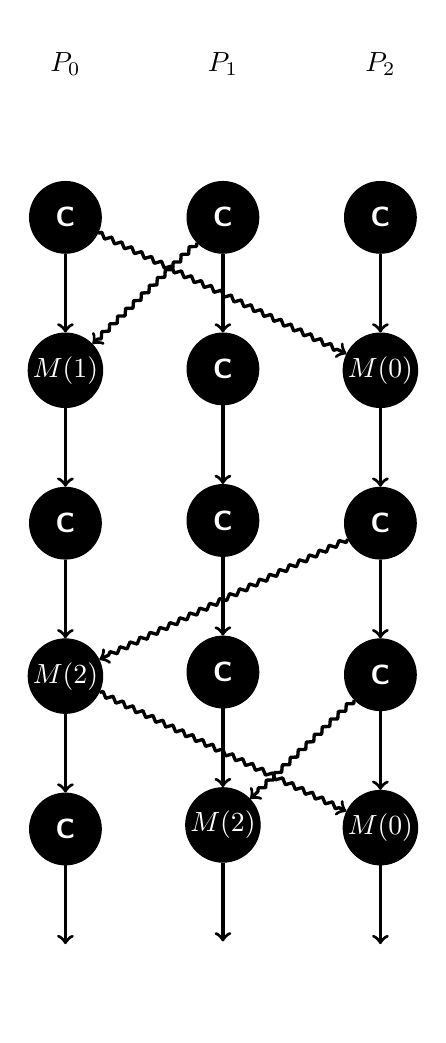
\begin{tikzpicture}
  \begin{scope}[start chain=2 going below,node distance= 1cm]
    \node [on chain=2,arn_bb,draw = none] {$P_0$};
    \node [on chain=2,arn_nb] (p00) {C};
    \node [on chain = 2,arn_nb] (p01) {$M(1)$};
    \node [on chain = 2,arn_nb] (p02) {C};
    \node [on chain = 2,arn_nb] (p03) {$M(2)$};
    \node [on chain=2,arn_nb] (p04) {C};
    \node [on chain=2,arn_bb,draw = none] (p05) {};
\end{scope}

\begin{scope}[shift={(2cm,0cm)},start chain=2 going below,node distance= 1cm]
\node [on chain=2,arn_bb,draw = none] {$P_1$};
    \node [on chain=2,arn_nb] (p10) {C};
    \node [on chain = 2,arn_nb] (p11) {C};
    \node [on chain = 2,arn_nb] (p12) {C};
    \node [on chain = 2,arn_nb] (p13) {C};
    \node [on chain=2,arn_nb] (p14) {$M(2)$};
    \node [on chain=2,arn_bb,draw = none] (p15) {};
\end{scope}

\begin{scope}[shift={(4cm,0cm)},start chain=2 going below,node distance= 1cm]
\node [on chain=2,arn_bb,draw = none] {$P_2$};
    \node [on chain=2,arn_nb] (p20) {C};
    \node [on chain = 2,arn_nb] (p21) {$M(0)$};
    \node [on chain = 2,arn_nb] (p22) {C};
    \node [on chain = 2,arn_nb] (p23) {C};
    \node [on chain=2,arn_nb] (p24) {$M(0)$};
    \node [on chain=2,arn_bb,draw = none] (p25) {};
\end{scope}
\draw[->,black,very thick] (p00.south) to (p01.north);
\draw[->,black,very thick] (p01.south) to (p02.north);
\draw[->,black,very thick] (p02.south) to (p03.north);
\draw[->,black,very thick] (p03.south) to (p04.north);
\draw[->,black,very thick] (p04.south) to (p05.north);


\draw[->,black,very thick] (p10.south) to (p11.north);
\draw[->,black,very thick] (p11.south) to (p12.north);
\draw[->,black,very thick] (p12.south) to (p13.north);
\draw[->,black,very thick] (p13.south) to (p14.north);
\draw[->,black,very thick] (p14.south) to (p15.north);

\draw[->,black,very thick] (p20.south) to (p21.north);
\draw[->,black,very thick] (p21.south) to (p22.north);
\draw[->,black,very thick] (p22.south) to (p23.north);
\draw[->,black,very thick] (p23.south) to (p24.north);
\draw[->,black,very thick] (p24.south) to (p25.north);

\draw[zigzag] (p10) to (p01);
\draw[zigzag] (p22) to (p03);
\draw[zigzag] (p23) to (p14);
\draw[zigzag] (p00) to (p21);
\draw[zigzag] (p03) to (p24);
 \end{tikzpicture}
 }
 \caption{Three processes sharing information} \label{fig:21}
\end{minipage}
\begin{minipage}{0.3\textwidth}
\centering
\scalebox{0.7}{
 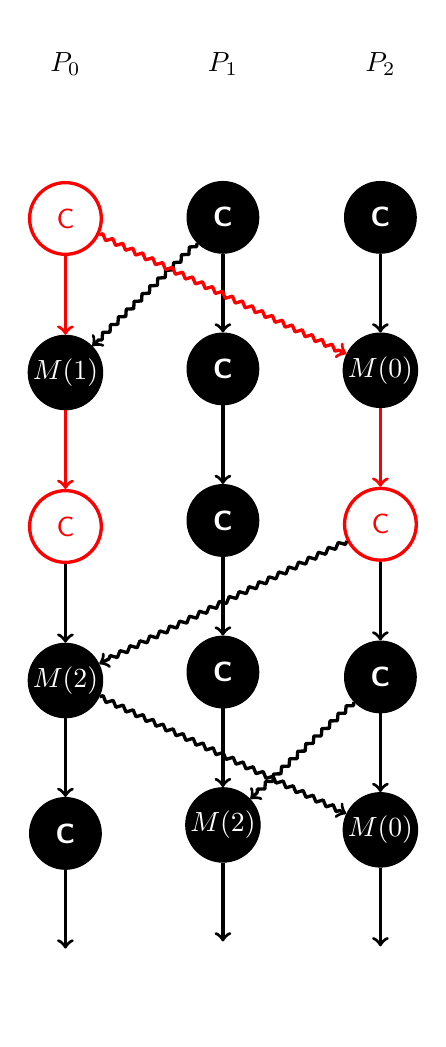
\begin{tikzpicture}
  \begin{scope}[start chain=2 going below,node distance= 1cm]
    \node [on chain=2,arn_bb,draw = none] {$P_0$};
    \node [on chain=2,arn_rb] (p00) {C};
    \node [on chain = 2,arn_nb] (p01) {$M(1)$};
    \node [on chain = 2,arn_rb] (p02) {C};
    \node [on chain = 2,arn_nb] (p03) {$M(2)$};
    \node [on chain=2,arn_nb] (p04) {C};
    \node [on chain=2,arn_bb,draw = none] (p05) {};
\end{scope}

\begin{scope}[shift={(2cm,0cm)},start chain=2 going below,node distance= 1cm]
\node [on chain=2,arn_bb,draw = none] {$P_1$};
    \node [on chain=2,arn_nb] (p10) {C};
    \node [on chain = 2,arn_nb] (p11) {C};
    \node [on chain = 2,arn_nb] (p12) {C};
    \node [on chain = 2,arn_nb] (p13) {C};
    \node [on chain=2,arn_nb] (p14) {$M(2)$};
    \node [on chain=2,arn_bb,draw = none] (p15) {};
\end{scope}

\begin{scope}[shift={(4cm,0cm)},start chain=2 going below,node distance= 1cm]
\node [on chain=2,arn_bb,draw = none] {$P_2$};
    \node [on chain=2,arn_nb] (p20) {C};
    \node [on chain = 2,arn_nb] (p21) {$M(0)$};
    \node [on chain = 2,arn_rb] (p22) {C};
    \node [on chain = 2,arn_nb] (p23) {C};
    \node [on chain=2,arn_nb] (p24) {$M(0)$};
    \node [on chain=2,arn_bb,draw = none] (p25) {};
\end{scope}
\draw[->,red,very thick] (p00.south) to (p01.north);
\draw[->,red,very thick] (p01.south) to (p02.north);
\draw[->,black,very thick] (p02.south) to (p03.north);
\draw[->,black,very thick] (p03.south) to (p04.north);
\draw[->,black,very thick] (p04.south) to (p05.north);


\draw[->,black,very thick] (p10.south) to (p11.north);
\draw[->,black,very thick] (p11.south) to (p12.north);
\draw[->,black,very thick] (p12.south) to (p13.north);
\draw[->,black,very thick] (p13.south) to (p14.north);
\draw[->,black,very thick] (p14.south) to (p15.north);

\draw[->,black,very thick] (p20.south) to (p21.north);
\draw[->,red,very thick] (p21.south) to (p22.north);
\draw[->,black,very thick] (p22.south) to (p23.north);
\draw[->,black,very thick] (p23.south) to (p24.north);
\draw[->,black,very thick] (p24.south) to (p25.north);

\draw[zigzag] (p10) to (p01);
\draw[zigzag] (p22) to (p03);
\draw[zigzag] (p23) to (p14);
\draw[zigzagred] (p00) to (p21);
\draw[zigzag] (p03) to (p24);
 \end{tikzpicture}
 }
 \caption{Biggest common ancestor between two nodes}  \label{fig:22}
\end{minipage}
\begin{minipage}{0.3\textwidth}
\centering
\scalebox{0.7}{
 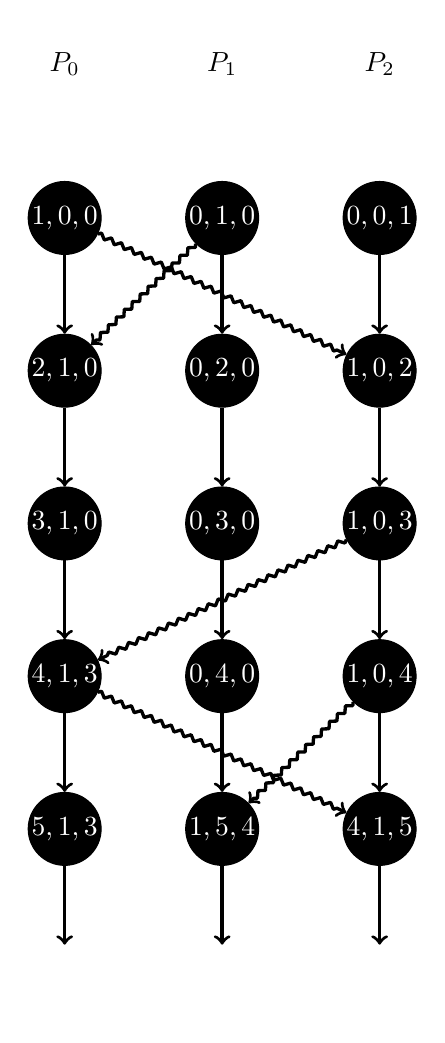
\begin{tikzpicture}
  \begin{scope}[start chain=2 going below,node distance= 1cm]
    \node [on chain=2,arn_bb,draw = none] {$P_0$};
    \node [on chain=2,arn_nb] (p00) {$1,0,0$};
    \node [on chain = 2,arn_nb] (p01) {$2,1,0$};
    \node [on chain = 2,arn_nb] (p02) {$3,1,0$};
    \node [on chain = 2,arn_nb] (p03) {$4,1,3$};
    \node [on chain=2,arn_nb] (p04) {$5,1,3$};
    \node [on chain=2,arn_bb,draw = none] (p05) {};
\end{scope}

\begin{scope}[shift={(2cm,0cm)},start chain=2 going below,node distance= 1cm]
\node [on chain=2,arn_bb,draw = none] {$P_1$};
    \node [on chain=2,arn_nb] (p10) {$0,1,0$};
    \node [on chain = 2,arn_nb] (p11) {$0,2,0$};
    \node [on chain = 2,arn_nb] (p12) {$0,3,0$};
    \node [on chain = 2,arn_nb] (p13) {$0,4,0$};
    \node [on chain=2,arn_nb] (p14) {$1,5,4$};
    \node [on chain=2,arn_bb,draw = none] (p15) {};
\end{scope}

\begin{scope}[shift={(4cm,0cm)},start chain=2 going below,node distance= 1cm]
\node [on chain=2,arn_bb,draw = none] {$P_2$};
    \node [on chain=2,arn_nb] (p20) {$0,0,1$};
    \node [on chain = 2,arn_nb] (p21) {$1,0,2$};
    \node [on chain = 2,arn_nb] (p22) {$1,0,3$};
    \node [on chain = 2,arn_nb] (p23) {$1,0,4$};
    \node [on chain=2,arn_nb] (p24) {$4,1,5$};
    \node [on chain=2,arn_bb,draw = none] (p25) {};
\end{scope}
\draw[->,black,very thick] (p00.south) to (p01.north);
\draw[->,black,very thick] (p01.south) to (p02.north);
\draw[->,black,very thick] (p02.south) to (p03.north);
\draw[->,black,very thick] (p03.south) to (p04.north);
\draw[->,black,very thick] (p04.south) to (p05.north);


\draw[->,black,very thick] (p10.south) to (p11.north);
\draw[->,black,very thick] (p11.south) to (p12.north);
\draw[->,black,very thick] (p12.south) to (p13.north);
\draw[->,black,very thick] (p13.south) to (p14.north);
\draw[->,black,very thick] (p14.south) to (p15.north);

\draw[->,black,very thick] (p20.south) to (p21.north);
\draw[->,black,very thick] (p21.south) to (p22.north);
\draw[->,black,very thick] (p22.south) to (p23.north);
\draw[->,black,very thick] (p23.south) to (p24.north);
\draw[->,black,very thick] (p24.south) to (p25.north);

\draw[zigzag] (p10) to (p01);
\draw[zigzag] (p22) to (p03);
\draw[zigzag] (p23) to (p14);
\draw[zigzag] (p00) to (p21);
\draw[zigzag] (p03) to (p24);
 \end{tikzpicture}
 }
 \caption{Labeling Nodes with partial order}  \label{fig:23}
\end{minipage}

\end{figure}

\paragraph{} The figure \ref{fig:21} shows an example with three processes doing commits (C) and Merging with other process ($M(i)$). This figure shows an underlying parial order between elements as defined by Leslie Lamport (TODO : put reference). We denote $\rightarrow$ a relation on states defined by : If $a$ and $b$ are two states of the same process $P_i$ and $a \prec_i b$ then $a \rightarrow b$. If $b$ is a merge state and $a$ is the state from which the merge occured on another process then $a \rightarrow b$. The $\rightarrow$ relation is closed under transitivity. We define the "Biggest common ancestors of $a$ and $b$" the set 
$\{c, 
c\rightarrow a 
\wedge 
c \rightarrow b 
\wedge 
\left ( 
\forall d\ ,
c \rightarrow d \Rightarrow \left ( d \nrightarrow a \vee d \nrightarrow b \right )
\right )
\}$. This set can be of any size, however \ref{fig:31} underlines what having two biggest common ancestors mean in term of merging. 
\paragraph{} Finding the biggest common ancestor(s) is an important problem when two processes want to merge, therefore it is interesting to find a way to discover quickly and without exchanging too many informations between two processes what are the biggest common ancestors of two nodes. For this purpose we label each of the states with a vector of integers of size $n$, $n$ being the total number of processes exchanging information. $\delta_i$ denotes the vector having zeros everywhere except a 1 at the $i$-th position. We build the label of the states in the "$\rightarrow$" order:
\begin{enumerate}
 \item If a state $a$ is a commit state on a process $P_i$ and as no predecessor for the $\prec_i$ relation then $a$ is labeled with $\delta_i$
 \item If a state $a$ is a commit state on a process $P_i$ and it has a biggest predecessor $b$ then $a$ is labeled with $\mathrm{label}(b) + \delta_i$
 \item If a state $a$ is a merge state with a state $b$ and $a$ as no predecessor for the $\prec_i$ relation then $a$ is labeled with $\mathrm{label}(b) + \delta_i$
 \item If a state $a$ is a merge state with a state $b$ and it has a biggest predecessor $c$ then $a$ is labeled with $\mathrm{max}(\mathrm{label}(b),\mathrm{label}(c)) + \delta_i$. Where $\max$ is the max on each component of the vector
\end{enumerate}
We define the $\leq$ relation on integer vector of size $n$ by : $u\leq v \Leftrightarrow \forall i \in \{0,\cdots,n-1\} u(i) \leq v(i)$ and $< := \leq \setminus =$. We have the following proposition on the labels of the states :
\begin{proposition}
 $ a \rightarrow b \Leftrightarrow \mathrm{label}(a) <  \mathrm{label}(b)$
\end{proposition}
\begin{proposition}
 If $c$ is the only biggest common ancestor of $a$ and $b$ then $\mathrm{label}(c) = \mathrm{min}(\mathrm{label}(a),\mathrm{label}(b))$
\end{proposition}



For the purpose of the introduction we will assume that for every two states we only have one biggest common ancestor.
\begin{figure}[H]
 \centering
 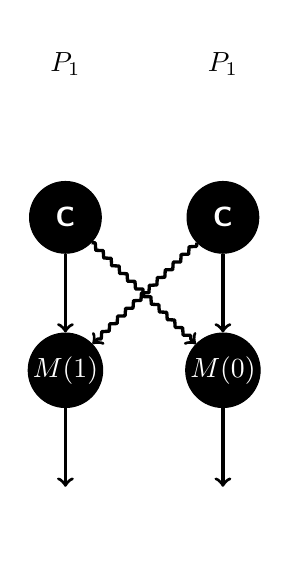
\begin{tikzpicture}
  \begin{scope}[shift={(2cm,0cm)},start chain=2 going below,node distance= 1cm]
\node [on chain=2,arn_bb,draw = none] {$P_1$};
    \node [on chain=2,arn_nb] (p10) {C};
    \node [on chain = 2,arn_nb] (p11) {$M(0)$};
    \node [on chain=2,arn_bb,draw = none] (p12) {};
    \end{scope}
    \begin{scope}[shift={(0cm,0cm)},start chain=2 going below,node distance= 1cm]
\node [on chain=2,arn_bb,draw = none] {$P_1$};
    \node [on chain=2,arn_nb] (p00) {C};
    \node [on chain = 2,arn_nb] (p01) {$M(1)$};
    \node [on chain=2,arn_bb,draw = none] (p02) {};
    \end{scope}
    
\draw[->,black,very thick] (p00.south) to (p01.north);
\draw[->,black,very thick] (p01.south) to (p02.north);
\draw[->,black,very thick] (p10.south) to (p11.north);
\draw[->,black,very thick] (p11.south) to (p12.north);

\draw[zigzag] (p00) to (p11);
\draw[zigzag] (p10) to (p01);
 \end{tikzpicture}
 \caption{Two biggest common ancestors} \label{fig:31}

\end{figure}

\section{Introduction to Bloom filters}
A Bloom filter is a space-efficient probabilistic Data structure that was conceived in 1970 by Burton Howard Bloom. This data structure is particularly efficient for adding an element or testing wether an element is in a set or not. This efficiency is at the cost of having some false positive but no false negative in the membership test. Here we will present the Bloom filters as they were used during my internship, however a lot of different variations have been used on bloomfilters. Let us consider a set $S' = \{x_0,\cdots,x_{n-1}\} \subset S$, we assume moreover that we have $k$ hash functions $\{h_0,\cdots,h_{k-1}\}$ from $S$ to $\{0,\cdots,m-1\}$ and a matrix $T$ of $m$ bits initially to zero. To store $S$ in our table, we change the table : $\forall i \in \{0,\cdots,n-1\},\ \forall j \in \{0,\cdots,k-1\},\ T(j)(h_j(x_i)) = 1$. To test the membership of $x$ in the Bloom filter we check wether $\forall i \in \{0,\cdots,n-1\},\ \forall j \in \{0,\cdots,k-1\},\ T(j)(h_j(x)) = 1$. This test can however raise false positive.
\begin{figure}[h]
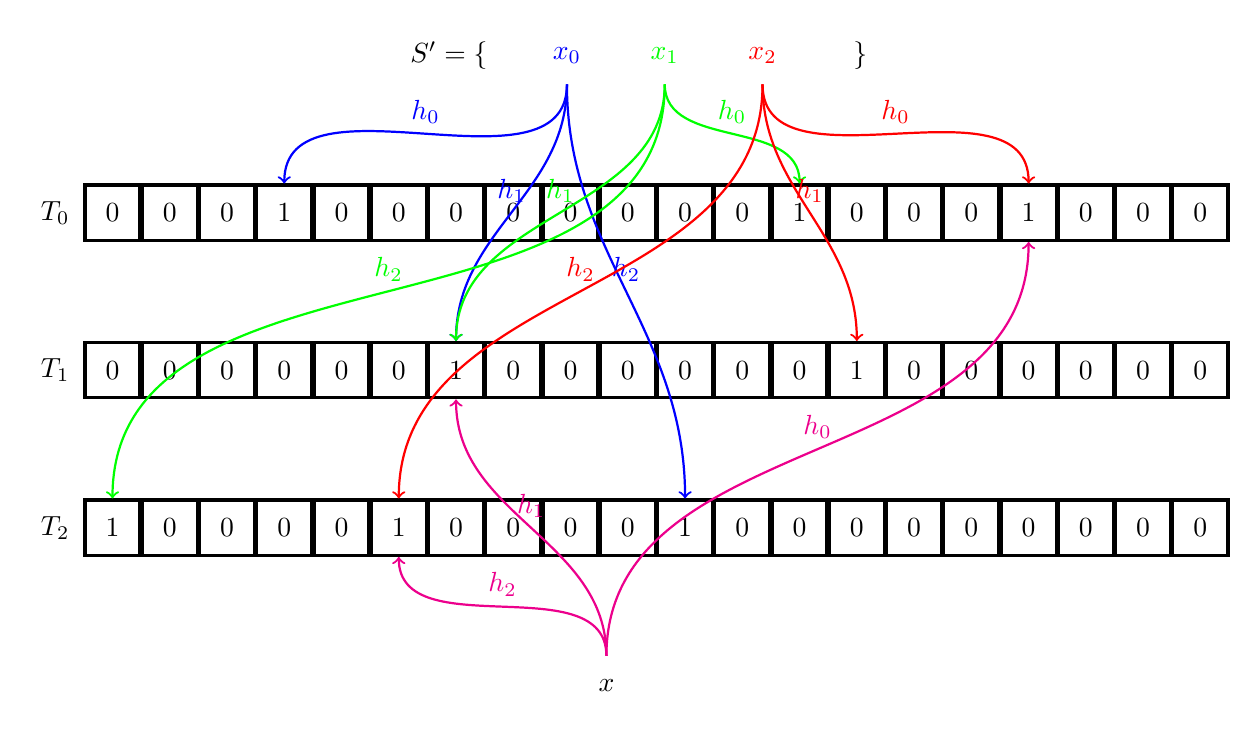
\begin{tikzpicture}
\tikzstyle{every path}=[very thick]

\edef\sizehash{0.7cm}
\tikzstyle{tmtape}=[draw,minimum size=\sizehash]

\begin{scope}[start chain=2 going right,node distance= 0.5cm]
    \node [on chain=2,tmtape,draw = none] {$S'=\{$};
    \node [on chain = 2,tmtape,draw = none] (x0) {\textcolor{blue}{$x_0$}};
    \node [on chain = 2,tmtape,draw = none] (x1) {\textcolor{green}{$x_1$}};
    \node [on chain = 2,tmtape,draw = none] (x2) {\textcolor{red}{$x_2$}};
    \node [on chain=2,tmtape,draw = none] {$\}$};
\end{scope}

\begin{scope}[shift={(-5cm,-2cm)},start chain=1 going right,node distance=-0.15mm]
    \node [on chain=1,tmtape,draw = none] {$T_0$};
    \node [on chain=1,tmtape] {$0$};
    \node [on chain=1,tmtape] {$0$};
    \node [on chain=1,tmtape] {$0$};
    \node [on chain=1,tmtape] (n0) {$1$};
    \node [on chain=1,tmtape] {$0$};
    \node [on chain=1,tmtape] {$0$};
    \node [on chain=1,tmtape] {$0$};
    \node [on chain=1,tmtape] {$0$};
    \node [on chain=1,tmtape] {$0$};
    \node [on chain=1,tmtape] {$0$};
    \node [on chain=1,tmtape] {$0$};
    \node [on chain=1,tmtape] {$0$};
    \node [on chain=1,tmtape] (n1) {$1$};
    \node [on chain=1,tmtape] {$0$};
    \node [on chain=1,tmtape] {$0$};
    \node [on chain=1,tmtape] {$0$};
    \node [on chain=1,tmtape] (n2) {$1$};
    \node [on chain=1,tmtape] {$0$};
    \node [on chain=1,tmtape] {$0$};
    \node [on chain=1,tmtape] {$0$};
\end{scope}

\begin{scope}[shift={(-5cm,-4cm)},start chain=1 going right,node distance=-0.15mm]
\node [on chain=1,tmtape,draw = none] {$T_1$};
    \node [on chain=1,tmtape] {$0$};
    \node [on chain=1,tmtape] {$0$};
    \node [on chain=1,tmtape] {$0$};
    \node [on chain=1,tmtape] {$0$};
    \node [on chain=1,tmtape] {$0$};
    \node [on chain=1,tmtape] {$0$};
    \node [on chain=1,tmtape] (n3) {$1$};
    \node [on chain=1,tmtape] {$0$};
    \node [on chain=1,tmtape] {$0$};
    \node [on chain=1,tmtape] {$0$};
    \node [on chain=1,tmtape] {$0$};
    \node [on chain=1,tmtape] {$0$};
    \node [on chain=1,tmtape] {$0$};
    \node [on chain=1,tmtape] (n4) {$1$};
    \node [on chain=1,tmtape] {$0$};
    \node [on chain=1,tmtape] {$0$};
    \node [on chain=1,tmtape] {$0$};
    \node [on chain=1,tmtape] {$0$};
    \node [on chain=1,tmtape] {$0$};
    \node [on chain=1,tmtape] {$0$};
\end{scope}
\begin{scope}[shift={(-5cm,-6cm)},start chain=1 going right,node distance=-0.15mm]
\node [on chain=1,tmtape,draw = none] {$T_2$};
    \node [on chain=1,tmtape] (n5) {$1$};
    \node [on chain=1,tmtape] {$0$};
    \node [on chain=1,tmtape] {$0$};
    \node [on chain=1,tmtape] {$0$};
    \node [on chain=1,tmtape] {$0$};
    \node [on chain=1,tmtape] (n6) {$1$};
    \node [on chain=1,tmtape] {$0$};
    \node [on chain=1,tmtape] {$0$};
    \node [on chain=1,tmtape] {$0$};
    \node [on chain=1,tmtape] {$0$};
    \node [on chain=1,tmtape] (n7) {$1$};
    \node [on chain=1,tmtape] {$0$};
    \node [on chain=1,tmtape] {$0$};
    \node [on chain=1,tmtape] {$0$};
    \node [on chain=1,tmtape] {$0$};
    \node [on chain=1,tmtape] {$0$};
    \node [on chain=1,tmtape] {$0$};
    \node [on chain=1,tmtape] {$0$};
    \node [on chain=1,tmtape] {$0$};
    \node [on chain=1,tmtape] {$0$};
\end{scope}
\begin{scope}[shift={(2cm,-8cm)},start chain=1 going right,node distance=-0.15mm]
\node [on chain=1,tmtape,draw = none] (x) {$x$};
\end{scope}

\draw[->,blue,thick] (x0.south) to[out=270,in=90] node[midway,above] {$h_0$} (n0.north);
\draw[->,blue,thick] (x0.south) to[out=270,in=90] node[midway,above] {$h_1$} (n3.north);
\draw[->,blue,thick] (x0.south) to[out=270,in=90] node[midway,above] {$h_2$} (n7.north);
\draw[->,green,thick] (x1.south) to[out=270,in=90] node[midway,above] {$h_0$} (n1.north);
\draw[->,green,thick] (x1.south) to[out=270,in=90] node[midway,above] {$h_1$} (n3.north);
\draw[->,green,thick] (x1.south) to[out=270,in=90] node[midway,above] {$h_2$} (n5.north);
\draw[->,red,thick] (x2.south) to[out=270,in=90] node[midway,above] {$h_0$} (n2.north);
\draw[->,red,thick] (x2.south) to[out=270,in=90] node[midway,above] {$h_1$} (n4.north);
\draw[->,red,thick] (x2.south) to[out=270,in=90] node[midway,above] {$h_2$} (n6.north);


\draw[->,magenta,thick] (x.north) to[out=90,in=270] node[midway,above] {$h_0$} (n2.south);
\draw[->,magenta,thick] (x.north) to[out=90,in=270] node[midway,above] {$h_1$} (n3.south);
\draw[->,magenta,thick] (x.north) to[out=90,in=270] node[midway,above] {$h_2$} (n6.south);
\end{tikzpicture}
\caption{Inserting and testing the membership in a Bloom Filter}
\end{figure}
\paragraph{}
\begin{proposition}
 Under the assumption that the set $\mathcal H$ is a set of size $k$ independant identically distributed hash functions ranging in $\{0,\cdots,m-1\}$, a table $T$ such as described before and a set $S'\subset S$  of size $n$ of elements inserted in $T$, then the probability $\mathbb{P}$ of having a false positive while testing $x \in S'$ is :
 \[
  \mathbb{P}=\left ( 1 - \left ( 1 - \frac{1}{m} \right )^n \right )^k
 \]
\end{proposition}
\begin{proof}
With the same notation than in the proposition :
 \begin{align*}
  \mathbb{P} &= \mathbb{P}(\forall j \in \{0,\cdots,k-1\}, T(j)(h_j(x)) = 1)\\
    &= \left ( \mathbb{P}(T(0)(h_0(x)) = 1) \right )^k\\
    &= \left ( \sum_{i=0}^{m-1} \mathbb{P}(T(0)(i) = 1)\mathbb{P}(h_0(x) = i)\right )^k\\
    &= \left ( \sum_{i=0}^{m-1} \mathbb{P}(T(0)(0) = 1)\frac{1}{m}\right )^k\\
    &= \left ( 1- \mathbb{P}(T(0)(0) = 0)\right )^k\\
    &= \left ( 1- \mathbb{P}(\forall p \in \{0,\cdots,n-1\} h_0(p) \neq 0 )\right )^k\\
    &= \left ( 1- \left ( \frac{m-1}{m} \right )^n \right )^k\\
 \end{align*}
\end{proof}


\chapter{Results}
\section{Preliminary result on DAGS and Bloom filters}
\label{sec:prelim}
As we change the problem from a finite and known number of process with at most one biggest common ancestor (BCA) to an unknown number of processes with no restriction on the number of BCA, it is important to study what will change and what do we have to expect regarding the number of BCA. Therefore using a DAG random generator (see section~\ref{sec:daggen}) we started by implementing the same algorithm that the one used on a finite and known number of process, except that we now assume that each node $a$ of the DAG contains a hash $h(a)$ of size $k$. We label every node $a$ of the tree with a vector $v(a)$ such that $v(a)_i=\sum_{b\in \mathrm{ancestor}(a)} h(b)_i$, with this labeling we test wether the proposition \ref{propmin} can still be used in some way. From the definition of the labeling we have :
\begin{proposition}
 If $c$ is a biggest common ancestor of $a$ and $b$ then $v(c) \leq \mathrm{min}(v(a),v(b))$. \label{propinf}
\end{proposition}
In our Dag algorithm nodes are placed in different layers, each layers having links only with the previous and the next one. An important parameter to consider is the probability for a node that a node from the previous layer is one of its parents. Examples of the influence of this parameter (called $p$) can be found in section~\ref{sec:daggen}. The "high" of a DAG is the length of the biggest path between two nodes of the DAG. The next graphs show the influence of $p$ and the high of the DAG on the number of BCA and on the number of element verifying the proposition \ref{propinf}.
\begin{figure}[H]
  \centering
 \begin{subfigure}[b]{0.49 \textwidth}
  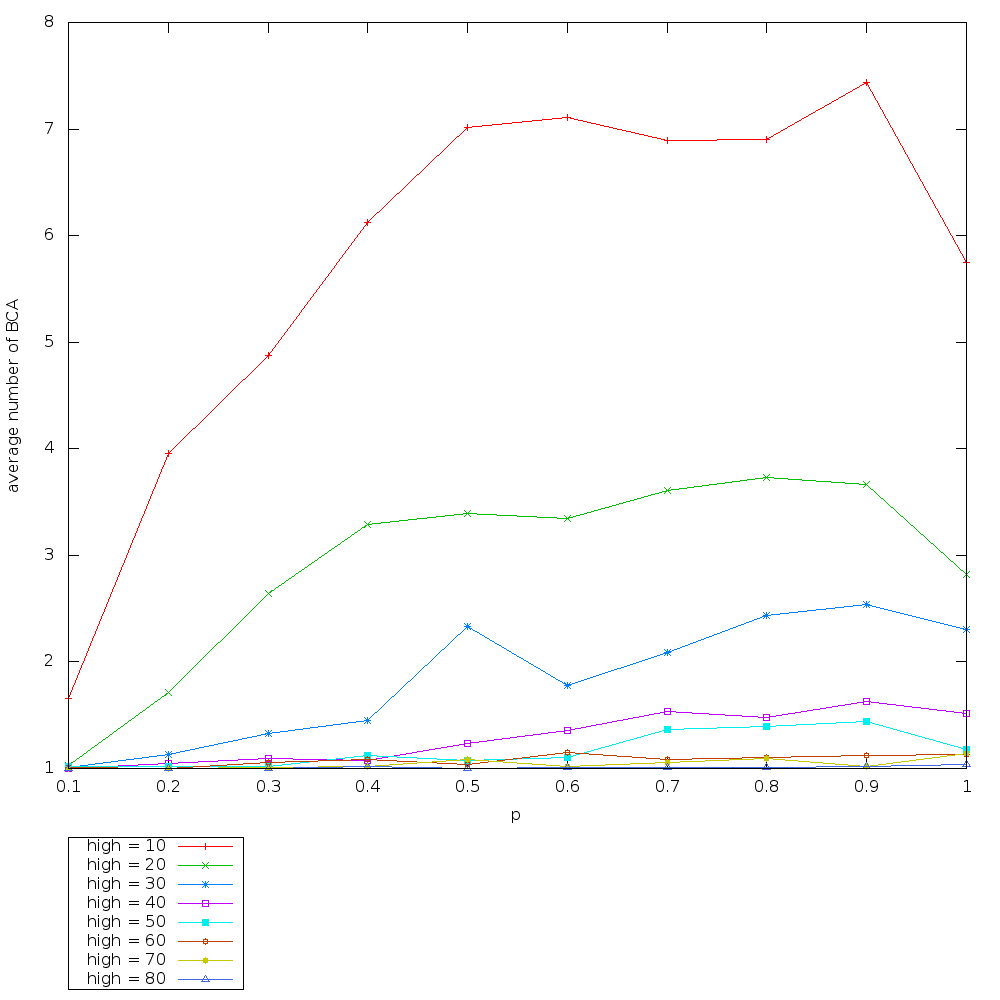
\includegraphics[width = \textwidth]{./image/resultprelim/averagenbbca.png}
  \caption{Number of Biggest Common Ancestor in a DAG with 100 nodes} \label{fig:nbbca}
 \end{subfigure}
 \begin{subfigure}[b]{0.49 \textwidth}
  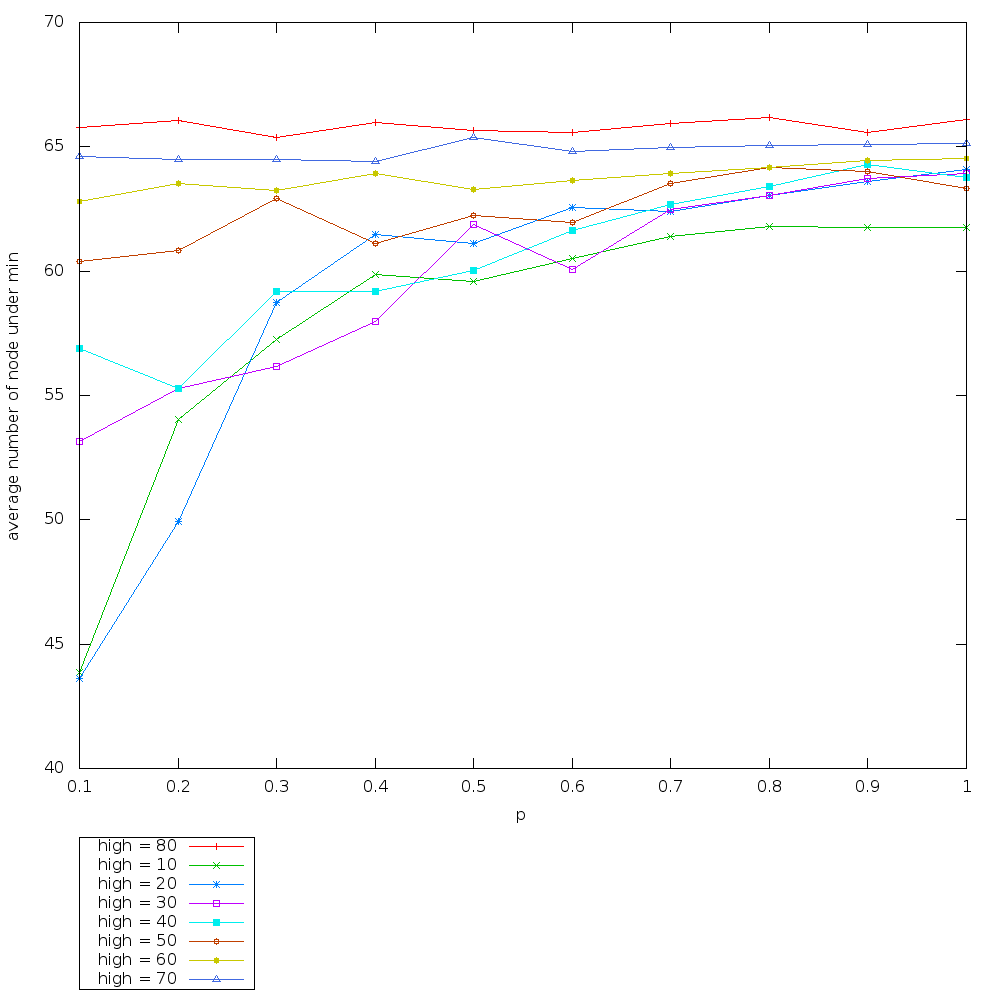
\includegraphics[width = \textwidth]{./image/resultprelim/averagenum.png}
  \caption{Number of element verifying the inequality of \ref{propinf} in a DAG with 100 nodes} \label{fig:num}
 \end{subfigure}
\end{figure}

Figure~\ref{fig:nbbca} underlines that the assumption on the number of biggest common ancestors was a strong assumption and that we can not rely on the case where there is only one BCA. Figure~\ref{fig:num} shows that adapting the algorithm from the case where we only have a finite and known number of processes might not be a good idea. Indeed we reduce the search of the biggest comman ancestor to $\frac{1}{3}$ of the DAG, but the size of the area to search remains linear in the size of the complete DAG.

\section{Algorithm}
\subsection{General algorithm}
In the following we will consider two DAGs, each with some particular nodes called head. The set of heads is the smallest set so that every node in the considered DAG is an ancestor of one of the head. One of the DAG will be refered to as Client or $Bob$ and the other one as Server or $Alice$. $\mathrm{Ancestor}(Alice)$ and $\mathrm{Ancestor}(Bob)$ are the considered DAGs and the aim of the algorithm is to be able to compute $\mathrm{Ancestor}(Alice) \setminus \mathrm{Ancestor}(Bob) = \{ x\ ,\ x \in \mathrm{Ancestor}(Alice) \wedge x \notin \mathrm{Ancestor}(Bob)\}$. The complexity of the algorithm will be expressed in terms of $n = \#(\mathrm{Ancestor}(Alice) \setminus \mathrm{Ancestor}(Bob))$. In terms of application, the client and the server are two entities that are physically distinct, therefore it was important during the design of the algorithm to keep in mind and to be aware that :
\begin{enumerate}
 \item The quantity of information exchanged between the two processes shall be the smaller possible
 \item We want to minimise the complexity on both processes
 \item There can be no no pre-assumptions on the shape of the graph, because the shape of the global DAG (with multiple head) is evolving in time and is not known at the beginning.
 \item There is no high authority that has a memory of every thing.
\end{enumerate}
\paragraph{} The section~\ref{sec:prelim} underlined that we were not able to find a way to compute easily the set of BCA, moreover if the server has to send the difference $\mathrm{Ancestor}(Alice) \setminus \mathrm{Ancestor}(Bob)$ then at some point we will have to go all over this difference, therefore we decided that the server could cross the part of its history corresponding to the difference.
% However the server does not know what nodes are already in the history of the client. Hence the client need to send to the server its history so that the server knows when the exploration of its past shal stop. Sending all of the client's history can requiere a huge exchange of data, moreover in applications we are interested in (git) the difference we are trying to compute is usually small compared to the size of the all history. the client shall therefore only send the latest event in its history (a fixed number) so that in most case the server manages to make the link between the two histories. However 
% in some cases the server will not be able to find any of the client's latest node in its history, in such cases the server will have to go throw all of its history (because the link can be anywhere) to understand that it has nothing in common with this set of latest nodes. We do not want the server to go throw all of its history as we have no bound on the size of this history. Thus the client need to tell the server that at some point of its exploration the server need to stop because there is no point in continuing the exploration. We introduce the Border of a set of nodes $A$ as defined such that for every nodes in $A$ each of its predecessor are either in $A$ or in the border of $A$. To sum up, the client divides its history in packages that will be called "window" and to each window we associate a "border" (see \ref{fig:twoproc}). Now if the client send a window and the union of all the borders to the server, this one will, at some point, find one of the two while exploring its history bottom-up and 
% therefore will not have to go across all of its history.
\begin{definition}
 Given a DAG $\mathcal{D}$ and a partition of a the nodes of $\mathcal{D}$, we call a set of equivalent nodes for this partition a "slice of $\mathcal{D}$"
\end{definition}
\begin{definition}
 Given a DAG $\mathcal{D}$ and a slice $\mathcal{S}$ we call the border of $\mathcal{S}$ (noted $\overline{\mathcal S}$)the smallest set such that $\forall x \in \mathcal{D},\ \forall y\in \mathrm{predecessor}{x} y\in \mathcal{S} \vee y \in \overline{\mathcal S}$.
\end{definition}
\paragraph{Idea of the algorithm} We assume that a partition of its DAG of ancestors is known by the client as well as well as a border for every slice of the partition.
\begin{enumerate}
 \item The client sends the list of its head, one of its slice and the union of all the border to the Server
 \item The server goes up in its history and stop whenever it crosses a node in the slice are in the border.
 \item The server computes the DAG $D$ of the successors of every nodes it found in slice.
 \item The server computes a list of "nodes of interest" from which it shall starts again the exploration (those "nodes of interest" are the last successors of the nodes found in the border that are not in $D$)
 \item The server sends back $D$ and the list of "nodes of interest"
 \item The client starts again with anoter slice and instead of the list of its head it sends the list of "nodes of interest" it received from the server, except if there is no "node of interest" in which case the algorithm stop.
\end{enumerate}
\paragraph{} This algorithm as the property that the server have absolutely no memory. The figure~\ref{fig:twoproc} shows a partition of two dags in slices.

\begin{figure}[H]
\centering
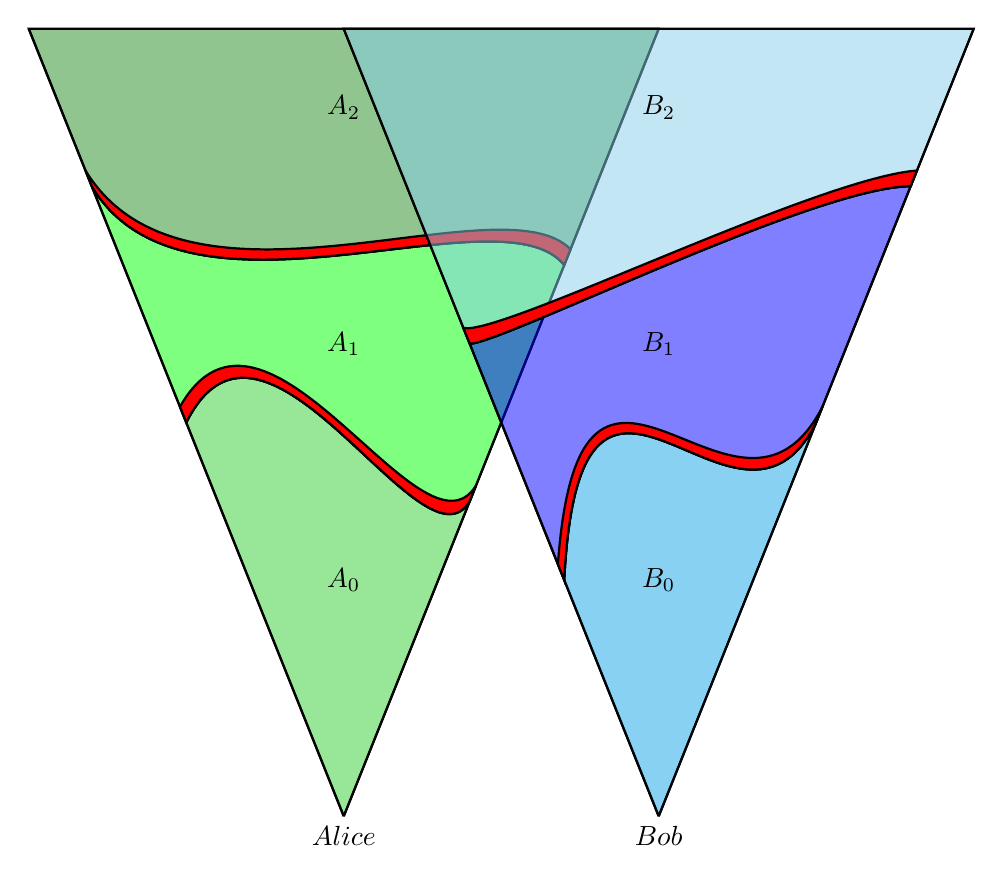
\begin{tikzpicture}
\begin{scope}
\coordinate[label=below:$Alice$] (A) at (0,0) ;
\coordinate (B) at (4,10);
\coordinate (C) at (-4,10);
\draw [thick] (A) -- (B) coordinate[pos = 0.4] (B1) {} coordinate [pos = 0.42] (B1b) {} coordinate[pos = 0.7] (B2) {} coordinate[pos = 0.72] (B2b) {};
\draw [thick] (B) -- (C) coordinate[pos = 0.5] (midBC) {};
\draw [thick] (A) -- (C) coordinate[pos = 0.5] (C1) {} coordinate [pos = 0.52] (C1b) {} coordinate[pos = 0.8] (C2) {} coordinate[pos = 0.82] (C2b) {};
\draw [thick, fill = LimeGreen,fill opacity = 0.5] (A) -- (B1) .. controls (1,3) and (-1,7) .. (C1) -- (A);
\draw [thick, fill = green,fill opacity = 0.5] (B1) .. controls (1,3) and (-1,7) .. (C1) -- (C2) .. controls (-2,6) and (2,8) .. (B2) -- (B1);
\draw [thick, fill = ForestGreen, fill opacity = 0.5] (C2) .. controls (-2,6) and (2,8) .. (B2) -- (B) -- (C) -- (C2);
\draw [thick, fill = red, fill opacity = 1] (B1b) .. controls (1,3.1) and (-1,7.1) .. (C1b) -- (C1) .. controls (-1,7) and (1,3) .. (B1) -- (B1b);
\draw [thick, fill = red, fill opacity = 1] (C2) .. controls (-2,6) and (2,8) .. (B2) -- (B2b) .. controls (2,8.1) and (-2,6.1) .. (C2b) -- (C2);
\draw [draw = none] (A) -- (midBC) node[pos = 0.3] {$A_0$} node[pos = 0.6] {$A_1$} node[pos = 0.9] {$A_2$};

\end{scope}
\begin{scope}[shift={(4cm,0cm)}]
\coordinate[label=below:$Bob$] (D) at (0,0);
\coordinate (E) at (4,10);
\coordinate (F) at (-4,10);
\draw [thick] (D) -- (E) coordinate[pos = 0.5] (E1) {} coordinate [pos = 0.52] (E1b) {} coordinate[pos = 0.8] (E2) {} coordinate[pos = 0.82] (E2b) {};
\draw [thick] (E) -- (F) coordinate[pos = 0.5] (midEF) {};
\draw [thick] (D) -- (F) coordinate[pos = 0.3] (F1) {} coordinate [pos = 0.32] (F1b) {} coordinate[pos = 0.6] (F2) {} coordinate[pos = 0.62] (F2b) {};
\draw [thick, fill = Cerulean,fill opacity = 0.5] (D) -- (E1) .. controls (1,3) and (-1,7) .. (F1) -- (D);
\draw [thick, fill = blue,fill opacity = 0.5] (E1) .. controls (1,3) and (-1,7) .. (F1) -- (F2) .. controls (-2,6) and (2,8) .. (E2) -- (E1);
\draw [thick, fill = SkyBlue, fill opacity = 0.5] (F2) .. controls (-2,6) and (2,8) .. (E2) -- (E) -- (F) -- (F2);
\draw [thick, fill = red, fill opacity = 1] (E1b) .. controls (1,3.1) and (-1,7.1) .. (F1b) -- (F1) .. controls (-1,7) and (1,3) .. (E1) -- (E1b);
\draw [thick, fill = red, fill opacity = 1] (F2) .. controls (-2,6) and (2,8) .. (E2) -- (E2b) .. controls (2,8.1) and (-2,6.1) .. (F2b) -- (F2);
\draw [draw = none] (D) -- (midEF) node[pos = 0.3] {$B_0$} node[pos = 0.6] {$B_1$} node[pos = 0.9] {$B_2$};
\end{scope}
\end{tikzpicture}
\caption{Two processes sharing a part of their history and their decomposition in Slices and Borders} \label{fig:twoproc}
\end{figure}
The figure~\ref{fig:twoproc} underlines the fact that it is interesting to have a interesting partition of the node, in the sense that :
\begin{enumerate}
 \item We want the borders to be small so that we do not have to send a lot of information
 \item We want to do the least sending/receiving data to/from the server possible
 \item We want those slices/border to be easy to compute, in the sense that we do not want to cross all of the history of the client each time we want to merge
 \item We want the slices to be all of the same size
\end{enumerate}
Let us assume we decided that the slices should be of size $n$ and that a process already knows a partition $\mathcal{P} = \{A_0,\cdots,A_m\}$ in slices of its ancestors and the paired borders. This process needs to add some nodes $S$ in its history. We start by filling the set in the partition with a size smaller that $n$, by adding the element from $S$ in an order verifying the order of the DAG. Therefore if $S$ contains two nodes $a$ and $b$, $a$ being a predecessor of $b$ then $a$ will be added prior than $b$. Once every partition is of size $n$ we add a new slice to $\mathcal P$. While adding a node in one of the slices we add it in the border if one of its parents is not in the slice. The order in which we add the elements ensures us that the border will be the small (regarding the number of element in the slice). Hence we can build a new partition and the corresponding borders quite easily from the previous one. Finally in order to ensure that there is not a lot of exchanges between the client and the server, the client send its slices from the newest to the oldest one. For example in figure~\ref{fig:twoproc} Bob will be sending the slices in the order $B_0$ then $B_1$ then $B_2$.
\begin{algorithm}[H] 
  \SetAlgoLined
  \caption{Finding some of the ancestors of $Alice$ not known by $Bob$}
  \SetKwInOut{Input}{input}\SetKwInOut{Output}{output}
  \SetKwComment{tcc}{(*}{*)}
  \KwData{\texttt{Alice\_Heads} : some nodes in the history of $Alice$, \texttt{Ancestor} : a dag of the ancesters of $Alice$, \texttt{G\_In} : a graph of ancestors of $Alice$ not known by $Bob$, \texttt{Bf} : The Bloom filter of $Bob$, \texttt{Bd} : The Border of $Bob$}
%   \KwData{
%     \begin{itemize}
%     \item \texttt{Alice\_Heads} : some nodes in the history of $Alice$
%     \item \texttt{Ancestor} : a dag of the ancesters of $Alice$
%     \item \texttt{G\_In} : a graph of ancestors of $Alice$ not known by $Bob$
%     \item \texttt{Bf} : The Bloom filter of $Bob$
%     \item \texttt{Bd} : The Border of $Bob$
%     \end{itemize}
%     }
  \KwResult{\texttt{G\_Out} : a graph of ancestors of $Alice$ not known by $Bob$, \texttt{node\_to\_check} : a list of ancestors of $Alice$ that shall be revisited with the next Bloomfilters}
%   \KwResult{
%   \begin{itemize}
%   \item \texttt{G\_Out} : a graph of ancestors of $Alice$ not known by $Bob$
%   \item \texttt{node\_to\_check} : a list of ancestors of $Alice$ that shall be revisited with the next Bloomfilters
%   \end{itemize}
%   }
  
\SetAlgoLined\DontPrintSemicolon
\SetKwFunction{explore}{\textbf{explore}}
\SetKwFunction{belong}{\textbf{belong}}
\SetKwFunction{addv}{\textbf{add\_vertex}}
\SetKwFunction{adde}{\textbf{add\_edge}}
\SetKwFunction{succ}{\textbf{successor}}
\SetKwFunction{pred}{\textbf{predecessor}}
\SetKwProg{myproc}{Procedure}{}{}
\myproc{\explore{\texttt{node},\texttt{visited},\texttt{in\_bf},\texttt{in\_border}}}{

  \eIf{\belong{\texttt{node,\texttt{Bf}}}}{
    \KwRet{(\texttt{visited} $\cup$ \texttt{node},\texttt{in\_bf} $\cup$ \texttt{node},\texttt{in\_border})}
  }
  {
    \eIf{\belong{\texttt{node,\texttt{Bd}}}}{
    \KwRet{(\texttt{visited} $\cup$ \texttt{node},\texttt{in\_bf} ,\texttt{in\_border}$\cup$ \texttt{node})}
    }
    {
      \texttt{visited\_already} = \texttt{node} $\cup$ \texttt{visited}\;
      \texttt{in\_bf\_already} = \texttt{in\_bf}\;				
      \texttt{in\_border\_already} = \texttt{in\_border}\;
      \For{\texttt{pere} $\in$ \pred{\texttt{Ancestor},\texttt{node}}}{
      \If{\texttt{pere} $\notin$ \texttt{explored}}
      {
	\texttt{visited\_already,in\_bf\_already,in\_border\_already} = \explore{\texttt{pere},\texttt{visited\_already},\texttt{in\_bf\_already},\texttt{in\_border\_already}}\;
      }
      }
      \KwRet{(\texttt{visited\_already},\texttt{in\_bf\_already},\texttt{in\_border\_already})}\;
    }	
  }
}

\SetKwFunction{bf}{\textbf{find\_in\_bf}}
\SetKwFunction{bd}{\textbf{find\_in\_border}}
\myproc{\bf{\texttt{node},\texttt{explored}}}{
    \addv{\texttt{G\_In},\texttt{node}}\;
    \texttt{already\_explored} = \texttt{explored} $\cup$ \texttt{node}\;
    \For{\texttt{fils} $\in$ \succ{\texttt{Ancestor},\texttt{node}}}{
      \adde{\texttt{G\_In},\texttt{node},\texttt{fils}}\;
      \If{$\texttt{fils} \notin \texttt{already\_explored} \wedge \texttt{fils} \notin \texttt{G\_In}$}{
	\texttt{already\_explored} = \bf{\texttt{fils},\texttt{already\_explored}}
	}
    }
    \KwRet{already\_explored}
}

\myproc{\bd{\texttt{node},\texttt{explored},\texttt{to\_further\_explore}}}{
  \If{$\texttt{node} \notin \texttt{explored}$}{
    \texttt{son\_in} = $\varnothing$\;
    \texttt{son\_out} = $\varnothing$\;
    \For{\texttt{fils} $\in$ \succ{\texttt{Ancestor},\texttt{node}}}{
      \eIf{\texttt{fils} $\in$ \texttt{G\_In}}{
	\texttt{son\_in} = \texttt{fils} $\cup$ \texttt{son\_in}\; 
      }{
	\texttt{son\_out} = \texttt{fils} $\cup$ \texttt{son\_out}\;
      }
    }
    \texttt{already\_explored} = \texttt{explored}\;
    \texttt{inter\_node} = \texttt{to\_further\_explore}\;
    \If{\texttt{son\_in} = $\varnothing$}{
      \texttt{inter\_node} = \texttt{node} $\cup$ \texttt{inter\_node}\;
    }
    \For{\texttt{fils} $\in$ \texttt{son\_out}}{
      \If{\texttt{fils} $\notin$ \texttt{already\_explored}}{
	\texttt{already\_explored},\texttt{inter\_node} = \bd{\texttt{fils},\texttt{already\_explored},\texttt{inter\_node}}\;
      }
    }
    \KwRet{(already\_explored,inter\_node)}\;
  }
}
\end{algorithm}
  \begin{algorithm}
  \SetAlgoLined
  \caption{Finding some of the ancestors of $Alice$ not known by $Bob$}
  \SetKwInOut{Input}{input}\SetKwInOut{Output}{output}
  \SetKwComment{tcc}{(*}{*)}
  \KwData{\texttt{Alice\_Heads} : some nodes in the history of $Alice$, \texttt{Ancestor} : a dag of the ancesters of $Alice$, \texttt{G\_In} : a graph of ancestors of $Alice$ not known by $Bob$, \texttt{Bf} : The Bloom filter of $Bob$, \texttt{Bd} : The Border of $Bob$}
%   \KwData{
%     \begin{itemize}
%     \item \texttt{Alice\_Heads} : some nodes in the history of $Alice$
%     \item \texttt{Ancestor} : a dag of the ancesters of $Alice$
%     \item \texttt{G\_In} : a graph of ancestors of $Alice$ not known by $Bob$
%     \item \texttt{Bf} : The Bloom filter of $Bob$
%     \item \texttt{Bd} : The Border of $Bob$
%     \end{itemize}
%     }
  \KwResult{\texttt{G\_Out} : a graph of ancestors of $Alice$ not known by $Bob$, \texttt{node\_to\_check} : a list of ancestors of $Alice$ that shall be revisited with the next Bloomfilters}
%   \KwResult{
%   \begin{itemize}
%   \item \texttt{G\_Out} : a graph of ancestors of $Alice$ not known by $Bob$
%   \item \texttt{node\_to\_check} : a list of ancestors of $Alice$ that shall be revisited with the next Bloomfilters
%   \end{itemize}
%   }
  
\SetAlgoLined\DontPrintSemicolon

  \texttt{explored} = $\varnothing$\;
  \texttt{in\_bf} = $\varnothing$\;
  \texttt{in\_border} = $\varnothing$\;
  \texttt{to\_further\_explore} = $\varnothing$\;
\SetKwFunction{explore}{\textbf{explore}}
\SetKwFunction{belong}{\textbf{belong}}
\SetKwFunction{addv}{\textbf{add\_vertex}}
\SetKwFunction{adde}{\textbf{add\_edge}}
\SetKwFunction{succ}{\textbf{successor}}
\SetKwFunction{pred}{\textbf{predecessor}}
\SetKwProg{myproc}{Procedure}{}{}
\myproc{\explore{\texttt{node}}}{

\If{\texttt{node} $\notin$ \texttt{explored}}
{
\texttt{explored} = \texttt{node} $\cup$ \texttt{explored}\;
\eIf{\belong{\texttt{node,\texttt{Bf}}}}{
  \texttt{in\_bf} = \texttt{node} $\cup$ \texttt{in\_bf}\;
  }
  {
  \eIf{\belong{\texttt{node,\texttt{Bd}}}}{
  \texttt{in\_border} = \texttt{node} $\cup$ \texttt{in\_border}\;
  }
  {
  \For{\texttt{pere} $\in$ \pred{\texttt{Ancestor},\texttt{node}}}{
    \explore{\texttt{pere}}
  }
  }
  }
}
}
\SetKwFunction{bf}{\textbf{find\_in\_bf}}
\SetKwFunction{bd}{\textbf{find\_in\_border}}
\myproc{\bf{\texttt{node}}}{
  \If{$\texttt{node} \notin \texttt{explored} \wedge \texttt{node} \notin \texttt{G\_In}$}{
    \addv{\texttt{G\_In},\texttt{node}}\;
    \For{\texttt{fils} $\in$ \succ{\texttt{Ancestor},\texttt{node}}}{
      \adde{\texttt{G\_In},\texttt{node},\texttt{fils}}\;
      \bf{\texttt{fils}}
    }
  }
}
\myproc{\bd{\texttt{node}}}{
  \If{$\texttt{node} \notin \texttt{explored}$}{
    \eIf{$\texttt{node} \in \texttt{G\_In}$}{
      \texttt{to\_further\_explore} = \texttt{node} $\cup$ \texttt{to\_further\_explore}\;
    }
    {
      \For{\texttt{fils} $\in$ \succ{\texttt{Ancestor},\texttt{node}}}{
      \bd{\texttt{fils}}
      }    
    }
  }
}
\For{\texttt{node} $\in$ \texttt{Alice\_Heads}}{
  \explore{\texttt{node}}
}
\texttt{explored} = $\varnothing$\;
\For{\texttt{node} $\in$ \texttt{in\_bf}}{
  \bf{\texttt{node}}
}
\texttt{explored} = $\varnothing$\;
\For{\texttt{node} $\in$ \texttt{in\_border}}{
  \bd{\texttt{node}}
}
\KwRet{(\texttt{G\_In,to\_further\_explore})}
  
  \end{algorithm}
  
  \begin{figure}[H]
  \begin{minipage}{0.3\textwidth}
  \centering
  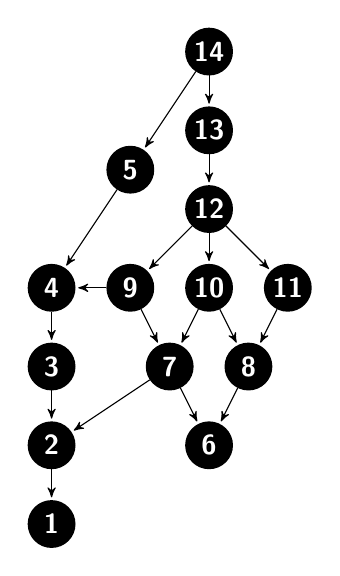
\begin{tikzpicture}[->,>=stealth',shorten >=1pt,auto,node distance=3cm,
  thick,main node/.style={circle,fill=blue!20,draw,font=\sffamily\Large\bfseries}]
  
  \foreach \place/\x in {{(0,0)/1}, {(0,1)/2},{(0,2)/3},{(0,3)/4}, {(1,4.5)/5}, {(2,1)/6}, {(1.5,2)/7},{(2.5,2)/8},{(1,3)/9},{(2,3)/10},{(3,3)/11},{(2,4)/12},{(2,5)/13},{(2,6)/14}}
  \node[arn_n] (a\x) at \place {\x};
%   Alice history
  \path[thin] (a14) edge (a5);
  \path[thin] (a5) edge (a4);
  \path[thin] (a4) edge (a3);
  \path[thin] (a3) edge (a2);
  \path[thin] (a2) edge (a1);
  \path[thin] (a9) edge (a4);
  \path[thin] (a7) edge (a2);
%   both history
  \path[thin] (a14) edge (a13);
  \path[thin] (a13) edge (a12);
  \path[thin] (a12) edge (a9);
  \path[thin] (a12) edge (a10);
  
  \path[thin] (a9) edge (a7);
  \path[thin] (a10) edge (a7);
%   Bob history
  \path[thin] (a12) edge (a11);
  \path[thin] (a11) edge (a8);
  \path[thin] (a10) edge (a8);
  \path[thin] (a7) edge (a6);
  \path[thin] (a8) edge (a6);
  \end{tikzpicture}
  \caption{Main Graph}
  \end{minipage}%
  \begin{minipage}{0.3\textwidth}
  \centering
  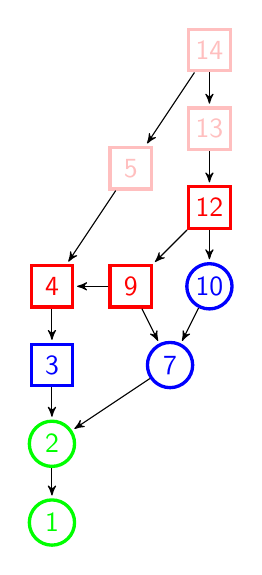
\begin{tikzpicture}[->,>=stealth',shorten >=1pt,auto,node distance=3cm,
  thick,main node/.style={circle,fill=blue!20,draw,font=\sffamily\Large\bfseries}]
  \foreach \place/\x in {{(0,0)/1}, {(0,1)/2}}
  \node[arn_g] (a\x) at \place {\x};
  
  
  \node[arn_pis] (a5) at (1,4.5) {5};
  \node[arn_pis] (a13) at (2,5) {13};
  \node[arn_pis] (a14) at (2,6) {14};
  
  
  \node[arn_b] (a10) at (2,3) {10};
  \node[arn_b] (a7) at (1.5,2) {7};
  \node[arn_bs] (a3) at (0,2) {3};
  
  \node[arn_rs] (a9) at (1,3) {9};
  \node[arn_rs] (a12) at (2,4) {12};
  \node[arn_rs] (a4) at (0,3) {4};
  %   Alice history
  \path[thin] (a14) edge (a5);
  \path[thin] (a5) edge (a4);
  \path[thin] (a4) edge (a3);
  \path[thin] (a3) edge (a2);
  \path[thin] (a2) edge (a1);
  \path[thin] (a9) edge (a4);
  \path[thin] (a7) edge (a2);
%   both history
  \path[thin] (a14) edge (a13);
  \path[thin] (a13) edge (a12);
  \path[thin] (a12) edge (a9);
  \path[thin] (a12) edge (a10);
  
  \path[thin] (a9) edge (a7);
  \path[thin] (a10) edge (a7);
  \end{tikzpicture}
  \caption{Alice's ancestors}
\end{minipage}%
\begin{minipage}{0.3\textwidth}
\centering
  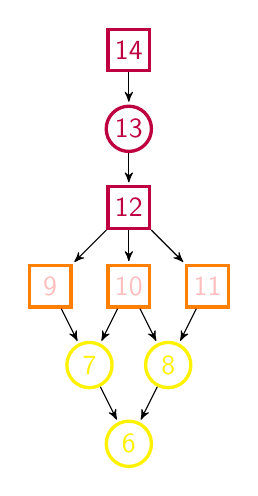
\begin{tikzpicture}[->,>=stealth',shorten >=1pt,auto,node distance=3cm,
  thick,main node/.style={circle,fill=blue!20,draw,font=\sffamily\Large\bfseries}]
%   
  \node[arn_y] (a6) at (2,1) {6};
  \node[arn_y] (a7) at (1.5,2) {7};
  \node[arn_y] (a8) at (2.5,2) {8};
  \node[arn_ts] (a9) at (1,3) {9};
  \node[arn_ts] (a10) at (2,3) {10};
  \node[arn_ts] (a11) at (3,3) {11};
  \node[arn_pus] (a12) at (2,4) {12};
  \node[arn_pu] (a13) at (2,5) {13};
  \node[arn_pus] (a14) at (2,6) {14};
  
%   both history
  \path[thin] (a14) edge (a13);
  \path[thin] (a13) edge (a12);
  \path[thin] (a12) edge (a9);
  \path[thin] (a12) edge (a10);
  
  \path[thin] (a9) edge (a7);
  \path[thin] (a10) edge (a7);
%   Bob history
  \path[thin] (a12) edge (a11);
  \path[thin] (a11) edge (a8);
  \path[thin] (a10) edge (a8);
  \path[thin] (a7) edge (a6);
  \path[thin] (a8) edge (a6);
  \end{tikzpicture}
  \caption{Bob's ancestors}

\end{minipage}
\end{figure}

\begin{figure}[H]
\begin{minipage}{0.3\textwidth}
\centering
 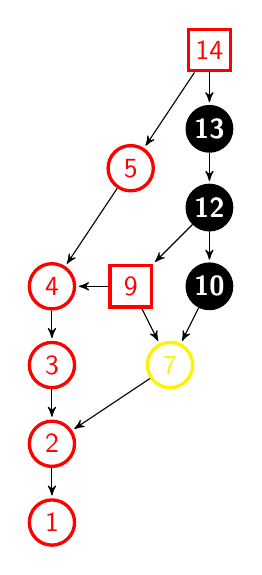
\begin{tikzpicture}[->,>=stealth',shorten >=1pt,auto,node distance=3cm,
  thick,main node/.style={circle,fill=blue!20,draw,font=\sffamily\Large\bfseries}]
  
  
  
  \node[arn_r] (a1) at (0,0) {1};
  \node[arn_r] (a2) at (0,1) {2};
  
  \node[arn_r] (a5) at (1,4.5) {5};
  \node[arn_n] (a13) at (2,5) {13};
  \node[arn_rs] (a14) at (2,6) {14};
  
  
  \node[arn_n] (a10) at (2,3) {10};
  \node[arn_y] (a7) at (1.5,2) {7};
  \node[arn_r] (a3) at (0,2) {3};
  
  \node[arn_rs] (a9) at (1,3) {9};
  \node[arn_n] (a12) at (2,4) {12};
  \node[arn_r] (a4) at (0,3) {4};
  
  %   Alice history
  \path[thin] (a14) edge (a5);
  \path[thin] (a5) edge (a4);
  \path[thin] (a4) edge (a3);
  \path[thin] (a3) edge (a2);
  \path[thin] (a2) edge (a1);
  \path[thin] (a9) edge (a4);
  \path[thin] (a7) edge (a2);
%   both history
  \path[thin] (a14) edge (a13);
  \path[thin] (a13) edge (a12);
  \path[thin] (a12) edge (a9);
  \path[thin] (a12) edge (a10);
  
  \path[thin] (a9) edge (a7);
  \path[thin] (a10) edge (a7);
  \end{tikzpicture}
  \caption*{[1] Explore}
\end{minipage}
\begin{minipage}{0.3\textwidth}
\centering
 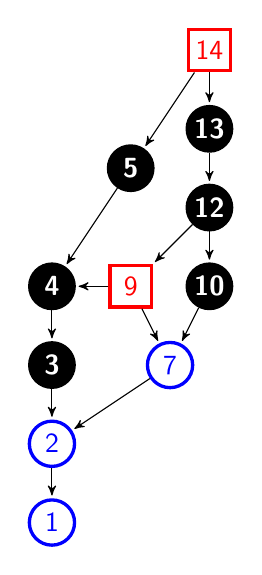
\begin{tikzpicture}[->,>=stealth',shorten >=1pt,auto,node distance=3cm,
  thick,main node/.style={circle,fill=blue!20,draw,font=\sffamily\Large\bfseries}]
  
  
  
  \node[arn_b] (a1) at (0,0) {1};
  \node[arn_b] (a2) at (0,1) {2};
  
  \node[arn_n] (a5) at (1,4.5) {5};
  \node[arn_n] (a13) at (2,5) {13};
  \node[arn_rs] (a14) at (2,6) {14};
  
  
  \node[arn_n] (a10) at (2,3) {10};
  \node[arn_b] (a7) at (1.5,2) {7};
  \node[arn_n] (a3) at (0,2) {3};
  
  \node[arn_rs] (a9) at (1,3) {9};
  \node[arn_n] (a12) at (2,4) {12};
  \node[arn_n] (a4) at (0,3) {4};
  
  %   Alice history
  \path[thin] (a14) edge (a5);
  \path[thin] (a5) edge (a4);
  \path[thin] (a4) edge (a3);
  \path[thin] (a3) edge (a2);
  \path[thin] (a2) edge (a1);
  \path[thin] (a9) edge (a4);
  \path[thin] (a7) edge (a2);
%   both history
  \path[thin] (a14) edge (a13);
  \path[thin] (a13) edge (a12);
  \path[thin] (a12) edge (a9);
  \path[thin] (a12) edge (a10);
  
  \path[thin] (a9) edge (a7);
  \path[thin] (a10) edge (a7);
  \end{tikzpicture}
  \caption{deal with bloomfilters}
\end{minipage}
 \begin{minipage}{0.3\textwidth}
 \centering
 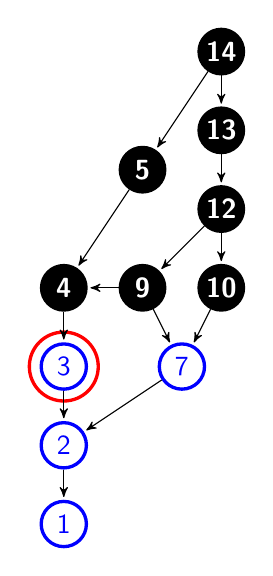
\begin{tikzpicture}[->,>=stealth',shorten >=1pt,auto,node distance=3cm,
  thick,main node/.style={circle,fill=blue!20,draw,font=\sffamily\Large\bfseries}]
  
  

  \node[arn_rb] (emph) at (0,2) {};
  \node[arn_b] (a1) at (0,0) {1};
  \node[arn_b] (a2) at (0,1) {2};
  
  \node[arn_n] (a5) at (1,4.5) {5};
  \node[arn_n] (a13) at (2,5) {13};
  \node[arn_n] (a14) at (2,6) {14};
  
  
  \node[arn_n] (a10) at (2,3) {10};
  \node[arn_b] (a7) at (1.5,2) {7};
  \node[arn_b] (a3) at (0,2) {3};
  
  \node[arn_n] (a9) at (1,3) {9};
  \node[arn_n] (a12) at (2,4) {12};
  \node[arn_n] (a4) at (0,3) {4};
%   \node[cloud, fill=gray!20, cloud puffs=16, cloud puff arc= 100,minimum width=2em, minimum height=2em, aspect=1] (cloud) at (5,2) {};

  %   Alice history
  \path[thin] (a14) edge (a5);
  \path[thin] (a5) edge (a4);
  \path[thin] (a4) edge (a3);
  \path[thin] (a3) edge (a2);
  \path[thin] (a2) edge (a1);
  \path[thin] (a9) edge (a4);
  \path[thin] (a7) edge (a2);
%   both history
  \path[thin] (a14) edge (a13);
  \path[thin] (a13) edge (a12);
  \path[thin] (a12) edge (a9);
  \path[thin] (a12) edge (a10);
  
  \path[thin] (a9) edge (a7);
  \path[thin] (a10) edge (a7);
  \end{tikzpicture}
  \caption{deal with border}
\end{minipage}
\end{figure}
\begin{figure}[H]
  \begin{minipage}{0.3\textwidth}
  \centering
 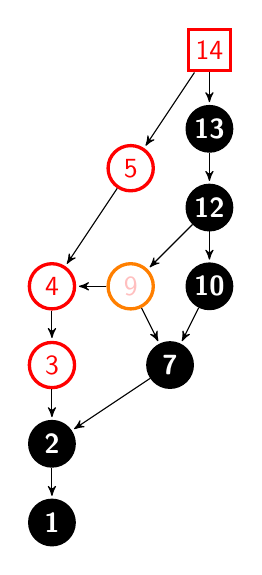
\begin{tikzpicture}[->,>=stealth',shorten >=1pt,auto,node distance=3cm,
  thick,main node/.style={circle,fill=blue!20,draw,font=\sffamily\Large\bfseries}]
  
  
  \node[arn_n] (a1) at (0,0) {1};
  \node[arn_n] (a2) at (0,1) {2};
  
  \node[arn_r] (a5) at (1,4.5) {5};
  \node[arn_n] (a13) at (2,5) {13};
  \node[arn_rs] (a14) at (2,6) {14};
  
  
  \node[arn_n] (a10) at (2,3) {10};
  \node[arn_n] (a7) at (1.5,2) {7};
  \node[arn_r] (a3) at (0,2) {3};
  
  \node[arn_t] (a9) at (1,3) {9};
  \node[arn_n] (a12) at (2,4) {12};
  \node[arn_r] (a4) at (0,3) {4};
%   \node[cloud, fill=gray!20, cloud puffs=16, cloud puff arc= 100,minimum width=2em, minimum height=2em, aspect=1] (cloud) at (5,2) {};

  %   Alice history
  \path[thin] (a14) edge (a5);
  \path[thin] (a5) edge (a4);
  \path[thin] (a4) edge (a3);
  \path[thin] (a3) edge (a2);
  \path[thin] (a2) edge (a1);
  \path[thin] (a9) edge (a4);
  \path[thin] (a7) edge (a2);
%   both history
  \path[thin] (a14) edge (a13);
  \path[thin] (a13) edge (a12);
  \path[thin] (a12) edge (a9);
  \path[thin] (a12) edge (a10);
  
  \path[thin] (a9) edge (a7);
  \path[thin] (a10) edge (a7);
  \end{tikzpicture}
  \caption{explore}
\end{minipage}
\begin{minipage}{0.3\textwidth}
  \centering
 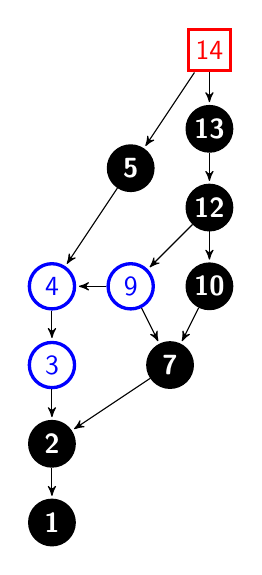
\begin{tikzpicture}[->,>=stealth',shorten >=1pt,auto,node distance=3cm,
  thick,main node/.style={circle,fill=blue!20,draw,font=\sffamily\Large\bfseries}]
  
  
  \node[arn_n] (a1) at (0,0) {1};
  \node[arn_n] (a2) at (0,1) {2};
  
  \node[arn_n] (a5) at (1,4.5) {5};
  \node[arn_n] (a13) at (2,5) {13};
  \node[arn_rs] (a14) at (2,6) {14};
  
  
  \node[arn_n] (a10) at (2,3) {10};
  \node[arn_n] (a7) at (1.5,2) {7};
  \node[arn_b] (a3) at (0,2) {3};
  
  \node[arn_b] (a9) at (1,3) {9};
  \node[arn_n] (a12) at (2,4) {12};
  \node[arn_b] (a4) at (0,3) {4};
%   \node[cloud, fill=gray!20, cloud puffs=16, cloud puff arc= 100,minimum width=2em, minimum height=2em, aspect=1] (cloud) at (5,2) {};

  %   Alice history
  \path[thin] (a14) edge (a5);
  \path[thin] (a5) edge (a4);
  \path[thin] (a4) edge (a3);
  \path[thin] (a3) edge (a2);
  \path[thin] (a2) edge (a1);
  \path[thin] (a9) edge (a4);
  \path[thin] (a7) edge (a2);
%   both history
  \path[thin] (a14) edge (a13);
  \path[thin] (a13) edge (a12);
  \path[thin] (a12) edge (a9);
  \path[thin] (a12) edge (a10);
  
  \path[thin] (a9) edge (a7);
  \path[thin] (a10) edge (a7);
  \end{tikzpicture}
  \caption{deal with bloomfilters}
\end{minipage}
\begin{minipage}{0.3\textwidth}
  \centering
 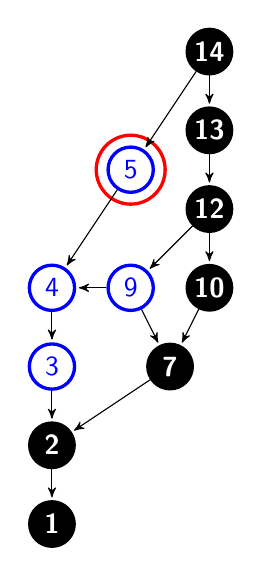
\begin{tikzpicture}[->,>=stealth',shorten >=1pt,auto,node distance=3cm,
  thick,main node/.style={circle,fill=blue!20,draw,font=\sffamily\Large\bfseries}]
  
  \node[arn_rb] (emph) at (1,4.5) {};
  \node[arn_n] (a1) at (0,0) {1};
  \node[arn_n] (a2) at (0,1) {2};
  
  \node[arn_b] (a5) at (1,4.5) {5};
  \node[arn_n] (a13) at (2,5) {13};
  \node[arn_n] (a14) at (2,6) {14};
  
  
  \node[arn_n] (a10) at (2,3) {10};
  \node[arn_n] (a7) at (1.5,2) {7};
  \node[arn_b] (a3) at (0,2) {3};
  
  \node[arn_b] (a9) at (1,3) {9};
  \node[arn_n] (a12) at (2,4) {12};
  \node[arn_b] (a4) at (0,3) {4};
%   \node[cloud, fill=gray!20, cloud puffs=16, cloud puff arc= 100,minimum width=2em, minimum height=2em, aspect=1] (cloud) at (5,2) {};

  %   Alice history
  \path[thin] (a14) edge (a5);
  \path[thin] (a5) edge (a4);
  \path[thin] (a4) edge (a3);
  \path[thin] (a3) edge (a2);
  \path[thin] (a2) edge (a1);
  \path[thin] (a9) edge (a4);
  \path[thin] (a7) edge (a2);
%   both history
  \path[thin] (a14) edge (a13);
  \path[thin] (a13) edge (a12);
  \path[thin] (a12) edge (a9);
  \path[thin] (a12) edge (a10);
  
  \path[thin] (a9) edge (a7);
  \path[thin] (a10) edge (a7);
  \end{tikzpicture}
  \caption{deal with borders}
\end{minipage}
\end{figure}
\begin{figure}[H]
 
\begin{minipage}{0.3\textwidth}
  \centering
 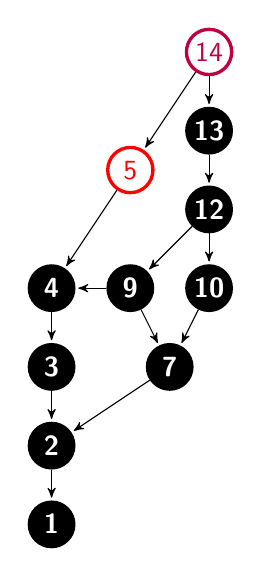
\begin{tikzpicture}[->,>=stealth',shorten >=1pt,auto,node distance=3cm,
  thick,main node/.style={circle,fill=blue!20,draw,font=\sffamily\Large\bfseries}]
  
  
  \node[arn_n] (a1) at (0,0) {1};
  \node[arn_n] (a2) at (0,1) {2};
  
  \node[arn_r] (a5) at (1,4.5) {5};
  \node[arn_n] (a13) at (2,5) {13};
  \node[arn_pu] (a14) at (2,6) {14};
  
  
  \node[arn_n] (a10) at (2,3) {10};
  \node[arn_n] (a7) at (1.5,2) {7};
  \node[arn_n] (a3) at (0,2) {3};
  
  \node[arn_n] (a9) at (1,3) {9};
  \node[arn_n] (a12) at (2,4) {12};
  \node[arn_n] (a4) at (0,3) {4};
%   \node[cloud, fill=gray!20, cloud puffs=16, cloud puff arc= 100,minimum width=2em, minimum height=2em, aspect=1] (cloud) at (5,2) {};

  %   Alice history
  \path[thin] (a14) edge (a5);
  \path[thin] (a5) edge (a4);
  \path[thin] (a4) edge (a3);
  \path[thin] (a3) edge (a2);
  \path[thin] (a2) edge (a1);
  \path[thin] (a9) edge (a4);
  \path[thin] (a7) edge (a2);
%   both history
  \path[thin] (a14) edge (a13);
  \path[thin] (a13) edge (a12);
  \path[thin] (a12) edge (a9);
  \path[thin] (a12) edge (a10);
  
  \path[thin] (a9) edge (a7);
  \path[thin] (a10) edge (a7);
  \end{tikzpicture}
  \caption{explore}
\end{minipage}
\begin{minipage}{0.3\textwidth}
  \centering
 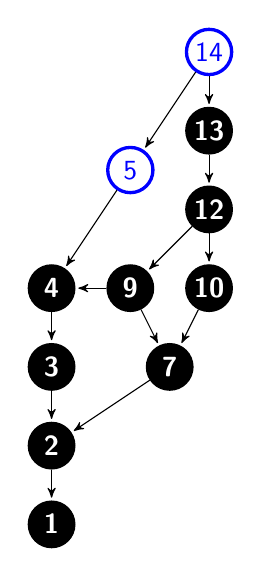
\begin{tikzpicture}[->,>=stealth',shorten >=1pt,auto,node distance=3cm,
  thick,main node/.style={circle,fill=blue!20,draw,font=\sffamily\Large\bfseries}]
  
  
  \node[arn_n] (a1) at (0,0) {1};
  \node[arn_n] (a2) at (0,1) {2};
  
  \node[arn_b] (a5) at (1,4.5) {5};
  \node[arn_n] (a13) at (2,5) {13};
  \node[arn_b] (a14) at (2,6) {14};
  
  
  \node[arn_n] (a10) at (2,3) {10};
  \node[arn_n] (a7) at (1.5,2) {7};
  \node[arn_n] (a3) at (0,2) {3};
  
  \node[arn_n] (a9) at (1,3) {9};
  \node[arn_n] (a12) at (2,4) {12};
  \node[arn_n] (a4) at (0,3) {4};
%   \node[cloud, fill=gray!20, cloud puffs=16, cloud puff arc= 100,minimum width=2em, minimum height=2em, aspect=1] (cloud) at (5,2) {};

  %   Alice history
  \path[thin] (a14) edge (a5);
  \path[thin] (a5) edge (a4);
  \path[thin] (a4) edge (a3);
  \path[thin] (a3) edge (a2);
  \path[thin] (a2) edge (a1);
  \path[thin] (a9) edge (a4);
  \path[thin] (a7) edge (a2);
%   both history
  \path[thin] (a14) edge (a13);
  \path[thin] (a13) edge (a12);
  \path[thin] (a12) edge (a9);
  \path[thin] (a12) edge (a10);
  
  \path[thin] (a9) edge (a7);
  \path[thin] (a10) edge (a7);
  \end{tikzpicture}
  \caption{deal with bloomfilters}
\end{minipage}
\begin{minipage}{0.3\textwidth}
  \centering
 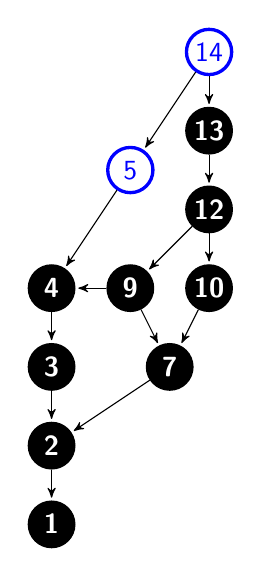
\begin{tikzpicture}[->,>=stealth',shorten >=1pt,auto,node distance=3cm,
  thick,main node/.style={circle,fill=blue!20,draw,font=\sffamily\Large\bfseries}]
  
  
  \node[arn_n] (a1) at (0,0) {1};
  \node[arn_n] (a2) at (0,1) {2};
  
  \node[arn_b] (a5) at (1,4.5) {5};
  \node[arn_n] (a13) at (2,5) {13};
  \node[arn_b] (a14) at (2,6) {14};
  
  
  \node[arn_n] (a10) at (2,3) {10};
  \node[arn_n] (a7) at (1.5,2) {7};
  \node[arn_n] (a3) at (0,2) {3};
  
  \node[arn_n] (a9) at (1,3) {9};
  \node[arn_n] (a12) at (2,4) {12};
  \node[arn_n] (a4) at (0,3) {4};
%   \node[cloud, fill=gray!20, cloud puffs=16, cloud puff arc= 100,minimum width=2em, minimum height=2em, aspect=1] (cloud) at (5,2) {};

  %   Alice history
  \path[thin] (a14) edge (a5);
  \path[thin] (a5) edge (a4);
  \path[thin] (a4) edge (a3);
  \path[thin] (a3) edge (a2);
  \path[thin] (a2) edge (a1);
  \path[thin] (a9) edge (a4);
  \path[thin] (a7) edge (a2);
%   both history
  \path[thin] (a14) edge (a13);
  \path[thin] (a13) edge (a12);
  \path[thin] (a12) edge (a9);
  \path[thin] (a12) edge (a10);
  
  \path[thin] (a9) edge (a7);
  \path[thin] (a10) edge (a7);
  \end{tikzpicture}
  \caption{deal with borders}
\end{minipage}
\end{figure}
\subsection{The False-positive case}
\label{sec:fp}
Our algorithm uses Bloom filters, therefore some false positive membership queries can happen, even if we chose the hash family so that the probibility that a false positive occurs is small. In the algorithm, membership queries only occur when the server is computing the difference between its history and the client one using Bloom filter. Let us consider that the server just received a Bloom filter and a list of "interesting nodes" from which it shall start exploring its ancestors, two different false positive cases can occur :
\begin{enumerate}
 \item A false positive occurs in a slice, therefore the server will stop exploring up at this node and will add all of its sons to the ring to send to the client. However the client will receive the ring and some node will not have any fathers in its history, those nodes shall be those in the "interesting nodes" list otherwise it means that it is a node the server considered in the history of the client and therefore can detect that a false positive occured. In such case the client can send back the same slice while signaling to the server which nodes were false-positive, hence the server will go accross the false-positive node and continue the exploration with the correct slice, for an example see \ref{bffp}.
 \item A false positive occurs in a border, there is no way to discover such a false positive until the end of the algorithm, when the client has sent all of its Bloom filters. At this point if the algorithm occured without any false positive, there should be no more "interesting nodes", however in the case of a false positive in a border, there remains some "interesting nodes". Considering that the border can not be trusted to test the membership, the client sends its border to the server that sends back to the client every nodes in its history that are ancestors of the remaining "interesting nodes" and that belongs to the client's border. The client verifies that the received nodes are in its history. If a node is not in its history, then it raised a false positive in the border, once we know all the false positive nodes, we send them to the server that will ignore them while starting over all of the exploration. We can notice that if a node was in the history of the client but was raising a false positive 
in the border, then we do not have a problem because the node was already in the client history, as were all of its ancestors, therefore we do not need this node to be further explored on the server side. Having a false positive in a border is a very rare case because the borders are rather small.
\end{enumerate}
\begin{figure}[H]
 \centering
 \resizebox{\textwidth}{!}{
 \begin{tabular}{c|c|c|c|c}
 \begin{subfigure}[b]{0.2\textwidth}
  \centering
  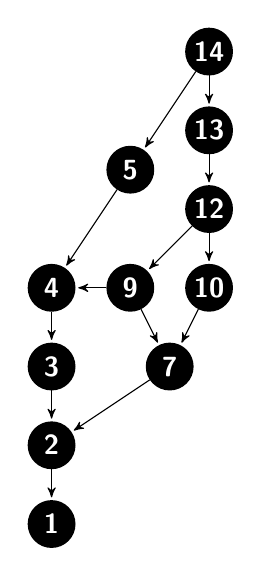
\begin{tikzpicture}[->,>=stealth',shorten >=1pt,auto,node distance=3cm,
  thick,main node/.style={circle,fill=blue!20,draw,font=\sffamily\Large\bfseries}]
  \foreach \place/\x in {{(0,0)/1}, {(0,1)/2}}
  \node[arn_n] (a\x) at \place {\x};
  
  
  \node[arn_n] (a5) at (1,4.5) {5};
  \node[arn_n] (a13) at (2,5) {13};
  \node[arn_n] (a14) at (2,6) {14};
  
  
  \node[arn_n] (a10) at (2,3) {10};
  \node[arn_n] (a7) at (1.5,2) {7};
  \node[arn_n] (a3) at (0,2) {3};
  
  \node[arn_n] (a9) at (1,3) {9};
  \node[arn_n] (a12) at (2,4) {12};
  \node[arn_n] (a4) at (0,3) {4};
  %   Alice history
  \path[thin] (a14) edge (a5);
  \path[thin] (a5) edge (a4);
  \path[thin] (a4) edge (a3);
  \path[thin] (a3) edge (a2);
  \path[thin] (a2) edge (a1);
  \path[thin] (a9) edge (a4);
  \path[thin] (a7) edge (a2);
%   both history
  \path[thin] (a14) edge (a13);
  \path[thin] (a13) edge (a12);
  \path[thin] (a12) edge (a9);
  \path[thin] (a12) edge (a10);
  
  \path[thin] (a9) edge (a7);
  \path[thin] (a10) edge (a7);
  \end{tikzpicture}
  \caption{Alice's ancestors}

  \end{subfigure}
  &
  \begin{subfigure}[b]{0.2\textwidth}
\centering
 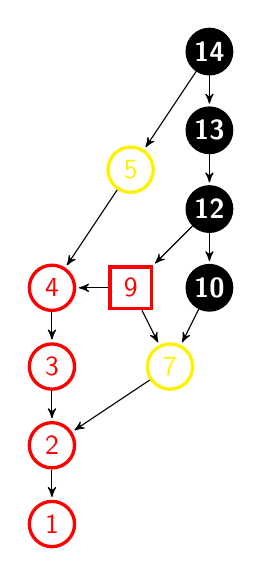
\begin{tikzpicture}[->,>=stealth',shorten >=1pt,auto,node distance=3cm,
  thick,main node/.style={circle,fill=blue!20,draw,font=\sffamily\Large\bfseries}]
  
  
  
  \node[arn_r] (a1) at (0,0) {1};
  \node[arn_r] (a2) at (0,1) {2};
  
  \node[arn_y] (a5) at (1,4.5) {5};
  \node[arn_n] (a13) at (2,5) {13};
  \node[arn_n] (a14) at (2,6) {14};
  
  
  \node[arn_n] (a10) at (2,3) {10};
  \node[arn_y] (a7) at (1.5,2) {7};
  \node[arn_r] (a3) at (0,2) {3};
  
  \node[arn_rs] (a9) at (1,3) {9};
  \node[arn_n] (a12) at (2,4) {12};
  \node[arn_r] (a4) at (0,3) {4};
  
  %   Alice history
  \path[thin] (a14) edge (a5);
  \path[thin] (a5) edge (a4);
  \path[thin] (a4) edge (a3);
  \path[thin] (a3) edge (a2);
  \path[thin] (a2) edge (a1);
  \path[thin] (a9) edge (a4);
  \path[thin] (a7) edge (a2);
%   both history
  \path[thin] (a14) edge (a13);
  \path[thin] (a13) edge (a12);
  \path[thin] (a12) edge (a9);
  \path[thin] (a12) edge (a10);
  
  \path[thin] (a9) edge (a7);
  \path[thin] (a10) edge (a7);
  \end{tikzpicture}
  \caption{Alice explores and 5 is a false positive}
\end{subfigure}
  &
  \begin{subfigure}[b]{0.2\textwidth}
 \centering
 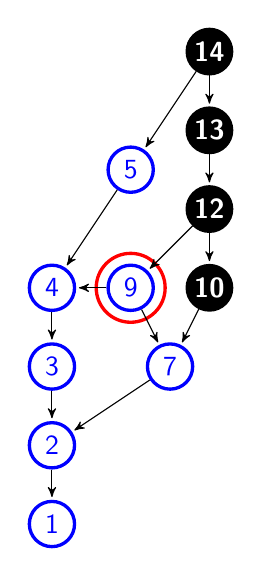
\begin{tikzpicture}[->,>=stealth',shorten >=1pt,auto,node distance=3cm,
  thick,main node/.style={circle,fill=blue!20,draw,font=\sffamily\Large\bfseries}]
  
  

  \node[arn_rb] (emph) at (1,3) {};
  \node[arn_b] (a1) at (0,0) {1};
  \node[arn_b] (a2) at (0,1) {2};
  
  \node[arn_b] (a5) at (1,4.5) {5};
  \node[arn_n] (a13) at (2,5) {13};
  \node[arn_n] (a14) at (2,6) {14};
  
  
  \node[arn_n] (a10) at (2,3) {10};
  \node[arn_b] (a7) at (1.5,2) {7};
  \node[arn_b] (a3) at (0,2) {3};
  
  \node[arn_b] (a9) at (1,3) {9};
  \node[arn_n] (a12) at (2,4) {12};
  \node[arn_b] (a4) at (0,3) {4};
%   \node[cloud, fill=gray!20, cloud puffs=16, cloud puff arc= 100,minimum width=2em, minimum height=2em, aspect=1] (cloud) at (5,2) {};

  %   Alice history
  \path[thin] (a14) edge (a5);
  \path[thin] (a5) edge (a4);
  \path[thin] (a4) edge (a3);
  \path[thin] (a3) edge (a2);
  \path[thin] (a2) edge (a1);
  \path[thin] (a9) edge (a4);
  \path[thin] (a7) edge (a2);
%   both history
  \path[thin] (a14) edge (a13);
  \path[thin] (a13) edge (a12);
  \path[thin] (a12) edge (a9);
  \path[thin] (a12) edge (a10);
  
  \path[thin] (a9) edge (a7);
  \path[thin] (a10) edge (a7);
  \end{tikzpicture}
  \caption{Alice deals with border and Bloom Filter nodes}
\end{subfigure}
&

  \begin{subfigure}[b]{0.2\textwidth}
 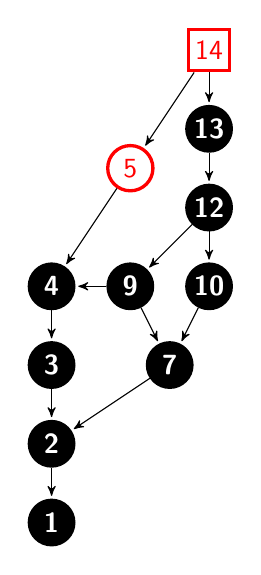
\begin{tikzpicture}[->,>=stealth',shorten >=1pt,auto,node distance=3cm,
  thick,main node/.style={circle,fill=blue!20,draw,font=\sffamily\Large\bfseries}]
  
  
  
  \node[arn_n] (a1) at (0,0) {1};
  \node[arn_n] (a2) at (0,1) {2};
  
  \node[arn_r] (a5) at (1,4.5) {5};
  \node[arn_n] (a13) at (2,5) {13};
  \node[arn_rs] (a14) at (2,6) {14};
  
  
  \node[arn_n] (a10) at (2,3) {10};
  \node[arn_n] (a7) at (1.5,2) {7};
  \node[arn_n] (a3) at (0,2) {3};
  
  \node[arn_n] (a9) at (1,3) {9};
  \node[arn_n] (a12) at (2,4) {12};
  \node[arn_n] (a4) at (0,3) {4};
  
  %   Alice history
  \path[thin] (a14) edge (a5);
  \path[thin] (a5) edge (a4);
  \path[thin] (a4) edge (a3);
  \path[thin] (a3) edge (a2);
  \path[thin] (a2) edge (a1);
  \path[thin] (a9) edge (a4);
  \path[thin] (a7) edge (a2);
%   both history
  \path[thin] (a14) edge (a13);
  \path[thin] (a13) edge (a12);
  \path[thin] (a12) edge (a9);
  \path[thin] (a12) edge (a10);
  
  \path[thin] (a9) edge (a7);
  \path[thin] (a10) edge (a7);
  \end{tikzpicture}
  \caption{Alice explores again starting at 5}
\end{subfigure}
&
  \begin{subfigure}[b]{0.2\textwidth}
 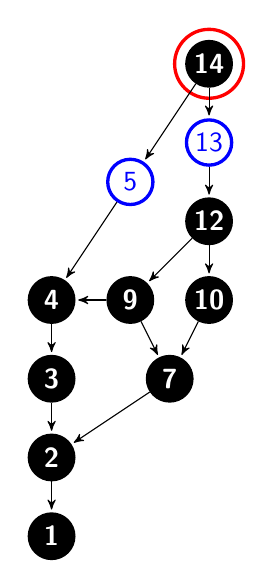
\begin{tikzpicture}[->,>=stealth',shorten >=1pt,auto,node distance=3cm,
  thick,main node/.style={circle,fill=blue!20,draw,font=\sffamily\Large\bfseries}]
  
  
   \node[arn_rb] (emph) at (2,6) {};
  \node[arn_n] (a1) at (0,0) {1};
  \node[arn_n] (a2) at (0,1) {2};
  
  \node[arn_b] (a5) at (1,4.5) {5};
  \node[arn_b] (a13) at (2,5) {13};
  \node[arn_n] (a14) at (2,6) {14};
  
  
  \node[arn_n] (a10) at (2,3) {10};
  \node[arn_n] (a7) at (1.5,2) {7};
  \node[arn_n] (a3) at (0,2) {3};
  
  \node[arn_n] (a9) at (1,3) {9};
  \node[arn_n] (a12) at (2,4) {12};
  \node[arn_n] (a4) at (0,3) {4};
  
  %   Alice history
  \path[thin] (a14) edge (a5);
  \path[thin] (a5) edge (a4);
  \path[thin] (a4) edge (a3);
  \path[thin] (a3) edge (a2);
  \path[thin] (a2) edge (a1);
  \path[thin] (a9) edge (a4);
  \path[thin] (a7) edge (a2);
%   both history
  \path[thin] (a14) edge (a13);
  \path[thin] (a13) edge (a12);
  \path[thin] (a12) edge (a9);
  \path[thin] (a12) edge (a10);
  
  \path[thin] (a9) edge (a7);
  \path[thin] (a10) edge (a7);
  \end{tikzpicture}
  \caption{Alice deals with Bloom filter and border nodes}
\end{subfigure}
  \\
    \begin{subfigure}[b]{0.2\textwidth}
\centering
  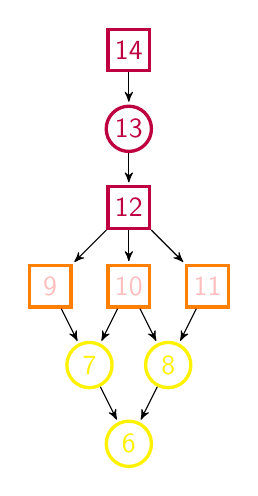
\begin{tikzpicture}[->,>=stealth',shorten >=1pt,auto,node distance=3cm,
  thick,main node/.style={circle,fill=blue!20,draw,font=\sffamily\Large\bfseries}]
%   
  \node[arn_y] (a6) at (2,1) {6};
  \node[arn_y] (a7) at (1.5,2) {7};
  \node[arn_y] (a8) at (2.5,2) {8};
  \node[arn_ts] (a9) at (1,3) {9};
  \node[arn_ts] (a10) at (2,3) {10};
  \node[arn_ts] (a11) at (3,3) {11};
  \node[arn_pus] (a12) at (2,4) {12};
  \node[arn_pu] (a13) at (2,5) {13};
  \node[arn_pus] (a14) at (2,6) {14};
  
%   both history
  \path[thin] (a14) edge (a13);
  \path[thin] (a13) edge (a12);
  \path[thin] (a12) edge (a9);
  \path[thin] (a12) edge (a10);
  
  \path[thin] (a9) edge (a7);
  \path[thin] (a10) edge (a7);
%   Bob history
  \path[thin] (a12) edge (a11);
  \path[thin] (a11) edge (a8);
  \path[thin] (a10) edge (a8);
  \path[thin] (a7) edge (a6);
  \path[thin] (a8) edge (a6);
  \end{tikzpicture}
  \caption{Bob's ancestors}
  \end{subfigure}
  &
  $\cdots$
  &
  \begin{subfigure}[b]{0.2\textwidth}
  \centering
  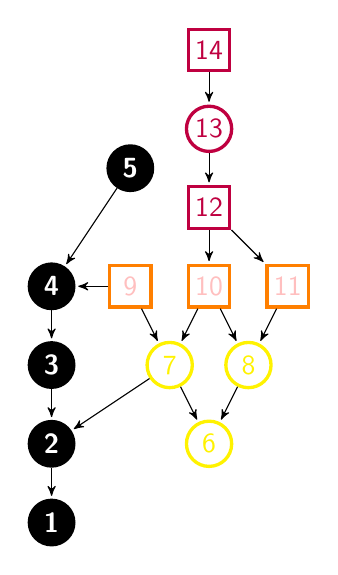
\begin{tikzpicture}[->,>=stealth',shorten >=1pt,auto,node distance=3cm,
  thick,main node/.style={circle,fill=blue!20,draw,font=\sffamily\Large\bfseries}]
  
  \foreach \place/\x in {{(0,0)/1}, {(0,1)/2},{(0,2)/3},{(0,3)/4}, {(1,4.5)/5}}
  \node[arn_n] (a\x) at \place {\x};
%   Alice history
%   \path[thin] (a14) edge (a5);
  \node[arn_y] (a6) at (2,1) {6};
  \node[arn_y] (a7) at (1.5,2) {7};
  \node[arn_y] (a8) at (2.5,2) {8};
  \node[arn_ts] (a9) at (1,3) {9};
  \node[arn_ts] (a10) at (2,3) {10};
  \node[arn_ts] (a11) at (3,3) {11};
  \node[arn_pus] (a12) at (2,4) {12};
  \node[arn_pu] (a13) at (2,5) {13};
  \node[arn_pus] (a14) at (2,6) {14};
  
  \path[thin] (a5) edge (a4);
  \path[thin] (a4) edge (a3);
  \path[thin] (a3) edge (a2);
  \path[thin] (a2) edge (a1);
  \path[thin] (a9) edge (a4);
  \path[thin] (a7) edge (a2);
%   both history
  \path[thin] (a14) edge (a13);
  \path[thin] (a13) edge (a12);
%   \path[thin] (a12) edge (a9);
  \path[thin] (a12) edge (a10);
  
  \path[thin] (a9) edge (a7);
  \path[thin] (a10) edge (a7);
%   Bob history
  \path[thin] (a12) edge (a11);
  \path[thin] (a11) edge (a8);
  \path[thin] (a10) edge (a8);
  \path[thin] (a7) edge (a6);
  \path[thin] (a8) edge (a6);
  \end{tikzpicture}
  \caption{Bob notices 5 should have a parent}
  \end{subfigure}
  &
  $\cdots$
  &
  \begin{subfigure}[b]{0.2\textwidth}
  \centering
  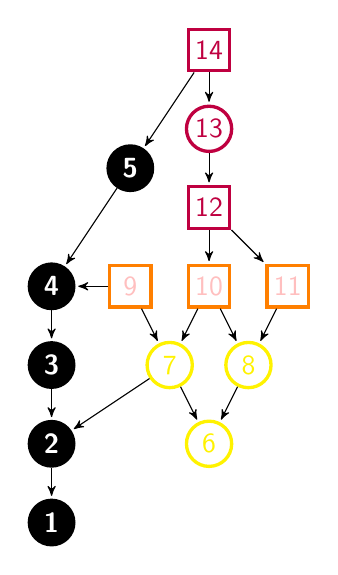
\begin{tikzpicture}[->,>=stealth',shorten >=1pt,auto,node distance=3cm,
  thick,main node/.style={circle,fill=blue!20,draw,font=\sffamily\Large\bfseries}]
  
  \foreach \place/\x in {{(0,0)/1}, {(0,1)/2},{(0,2)/3},{(0,3)/4}, {(1,4.5)/5}}
  \node[arn_n] (a\x) at \place {\x};
%   Alice history
%   \path[thin] (a14) edge (a5);
  \node[arn_y] (a6) at (2,1) {6};
  \node[arn_y] (a7) at (1.5,2) {7};
  \node[arn_y] (a8) at (2.5,2) {8};
  \node[arn_ts] (a9) at (1,3) {9};
  \node[arn_ts] (a10) at (2,3) {10};
  \node[arn_ts] (a11) at (3,3) {11};
  \node[arn_pus] (a12) at (2,4) {12};
  \node[arn_pu] (a13) at (2,5) {13};
  \node[arn_pus] (a14) at (2,6) {14};
  
  \path[thin] (a5) edge (a4);
  \path[thin] (a4) edge (a3);
  \path[thin] (a3) edge (a2);
  \path[thin] (a2) edge (a1);
  \path[thin] (a9) edge (a4);
  \path[thin] (a7) edge (a2);
%   both history
  \path[thin] (a14) edge (a5);
  \path[thin] (a14) edge (a13);
  \path[thin] (a13) edge (a12);
%   \path[thin] (a12) edge (a9);
  \path[thin] (a12) edge (a10);
  
  \path[thin] (a9) edge (a7);
  \path[thin] (a10) edge (a7);
%   Bob history
  \path[thin] (a12) edge (a11);
  \path[thin] (a11) edge (a8);
  \path[thin] (a10) edge (a8);
  \path[thin] (a7) edge (a6);
  \path[thin] (a8) edge (a6);
  \end{tikzpicture}
  \caption{Bob notices 5 should have a parent}
  \end{subfigure}
  \end{tabular}
}
\caption{How a false positive in a Bloom filter is detected and dealt with} \label{bffp}
\end{figure}

% \begin{figure}[H]
%  \centering
%   \begin{subfigure}[b]{0.2\textwidth}
%   \centering
%   \begin{tikzpicture}[->,>=stealth',shorten >=1pt,auto,node distance=3cm,
%   thick,main node/.style={circle,fill=blue!20,draw,font=\sffamily\Large\bfseries}]
%   \foreach \place/\x in {{(0,0)/1}, {(0,1)/2}}
%   \node[arn_n] (a\x) at \place {\x};
%   
%   
%   \node[arn_n] (a5) at (1,4.5) {5};
%   \node[arn_n] (a13) at (2,5) {13};
%   \node[arn_n] (a14) at (2,6) {14};
%   
%   
%   \node[arn_n] (a10) at (2,3) {10};
%   \node[arn_n] (a7) at (1.5,2) {7};
%   \node[arn_n] (a3) at (0,2) {3};
%   
%   \node[arn_n] (a9) at (1,3) {9};
%   \node[arn_n] (a12) at (2,4) {12};
%   \node[arn_n] (a4) at (0,3) {4};
%   %   Alice history
%   \path[thin] (a14) edge (a5);
%   \path[thin] (a5) edge (a4);
%   \path[thin] (a4) edge (a3);
%   \path[thin] (a3) edge (a2);
%   \path[thin] (a2) edge (a1);
%   \path[thin] (a9) edge (a4);
%   \path[thin] (a7) edge (a2);
% %   both history
%   \path[thin] (a14) edge (a13);
%   \path[thin] (a13) edge (a12);
%   \path[thin] (a12) edge (a9);
%   \path[thin] (a12) edge (a10);
%   
%   \path[thin] (a9) edge (a7);
%   \path[thin] (a10) edge (a7);
%   \end{tikzpicture}
%   \caption{Alice's ancestors}
% 
%   \end{subfigure}
%   \begin{subfigure}[b]{0.2\textwidth}
% \centering
%   \begin{tikzpicture}[->,>=stealth',shorten >=1pt,auto,node distance=3cm,
%   thick,main node/.style={circle,fill=blue!20,draw,font=\sffamily\Large\bfseries}]
% %   
%   \node[arn_y] (a6) at (2,1) {6};
%   \node[arn_y] (a7) at (1.5,2) {7};
%   \node[arn_y] (a8) at (2.5,2) {8};
%   \node[arn_ts] (a9) at (1,3) {9};
%   \node[arn_ts] (a10) at (2,3) {10};
%   \node[arn_ts] (a11) at (3,3) {11};
%   \node[arn_pus] (a12) at (2,4) {12};
%   \node[arn_pu] (a13) at (2,5) {13};
%   \node[arn_pus] (a14) at (2,6) {14};
%   
% %   both history
%   \path[thin] (a14) edge (a13);
%   \path[thin] (a13) edge (a12);
%   \path[thin] (a12) edge (a9);
%   \path[thin] (a12) edge (a10);
%   
%   \path[thin] (a9) edge (a7);
%   \path[thin] (a10) edge (a7);
% %   Bob history
%   \path[thin] (a12) edge (a11);
%   \path[thin] (a11) edge (a8);
%   \path[thin] (a10) edge (a8);
%   \path[thin] (a7) edge (a6);
%   \path[thin] (a8) edge (a6);
%   \end{tikzpicture}
%   \caption{Bob's ancestors}
%   \end{subfigure}
% \begin{subfigure}[b]{0.2\textwidth}
% \centering
%  \begin{tikzpicture}[->,>=stealth',shorten >=1pt,auto,node distance=3cm,
%   thick,main node/.style={circle,fill=blue!20,draw,font=\sffamily\Large\bfseries}]
%   
%   
%   
%   \node[arn_r] (a1) at (0,0) {1};
%   \node[arn_r] (a2) at (0,1) {2};
%   
%   \node[arn_y] (a5) at (1,4.5) {5};
%   \node[arn_n] (a13) at (2,5) {13};
%   \node[arn_n] (a14) at (2,6) {14};
%   
%   
%   \node[arn_n] (a10) at (2,3) {10};
%   \node[arn_y] (a7) at (1.5,2) {7};
%   \node[arn_r] (a3) at (0,2) {3};
%   
%   \node[arn_rs] (a9) at (1,3) {9};
%   \node[arn_n] (a12) at (2,4) {12};
%   \node[arn_r] (a4) at (0,3) {4};
%   
%   %   Alice history
%   \path[thin] (a14) edge (a5);
%   \path[thin] (a5) edge (a4);
%   \path[thin] (a4) edge (a3);
%   \path[thin] (a3) edge (a2);
%   \path[thin] (a2) edge (a1);
%   \path[thin] (a9) edge (a4);
%   \path[thin] (a7) edge (a2);
% %   both history
%   \path[thin] (a14) edge (a13);
%   \path[thin] (a13) edge (a12);
%   \path[thin] (a12) edge (a9);
%   \path[thin] (a12) edge (a10);
%   
%   \path[thin] (a9) edge (a7);
%   \path[thin] (a10) edge (a7);
%   \end{tikzpicture}
%   \caption{Alice explores and 5 is a false positive}
% \end{subfigure}
%  \begin{subfigure}[b]{0.2\textwidth}
%  \centering
%  \begin{tikzpicture}[->,>=stealth',shorten >=1pt,auto,node distance=3cm,
%   thick,main node/.style={circle,fill=blue!20,draw,font=\sffamily\Large\bfseries}]
%   
%   
% 
%   \node[arn_rb] (emph) at (1,3) {};
%   \node[arn_b] (a1) at (0,0) {1};
%   \node[arn_b] (a2) at (0,1) {2};
%   
%   \node[arn_b] (a5) at (1,4.5) {5};
%   \node[arn_n] (a13) at (2,5) {13};
%   \node[arn_n] (a14) at (2,6) {14};
%   
%   
%   \node[arn_n] (a10) at (2,3) {10};
%   \node[arn_b] (a7) at (1.5,2) {7};
%   \node[arn_b] (a3) at (0,2) {3};
%   
%   \node[arn_b] (a9) at (1,3) {9};
%   \node[arn_n] (a12) at (2,4) {12};
%   \node[arn_b] (a4) at (0,3) {4};
% %   \node[cloud, fill=gray!20, cloud puffs=16, cloud puff arc= 100,minimum width=2em, minimum height=2em, aspect=1] (cloud) at (5,2) {};
% 
%   %   Alice history
%   \path[thin] (a14) edge (a5);
%   \path[thin] (a5) edge (a4);
%   \path[thin] (a4) edge (a3);
%   \path[thin] (a3) edge (a2);
%   \path[thin] (a2) edge (a1);
%   \path[thin] (a9) edge (a4);
%   \path[thin] (a7) edge (a2);
% %   both history
%   \path[thin] (a14) edge (a13);
%   \path[thin] (a13) edge (a12);
%   \path[thin] (a12) edge (a9);
%   \path[thin] (a12) edge (a10);
%   
%   \path[thin] (a9) edge (a7);
%   \path[thin] (a10) edge (a7);
%   \end{tikzpicture}
%   \caption{Alice deals with border and Bloom Filter nodes}
% \end{subfigure}
%  \begin{subfigure}{0.2\textwidth}
%   \centering
%   \begin{tikzpicture}[->,>=stealth',shorten >=1pt,auto,node distance=3cm,
%   thick,main node/.style={circle,fill=blue!20,draw,font=\sffamily\Large\bfseries}]
%   
%   \foreach \place/\x in {{(0,0)/1}, {(0,1)/2},{(0,2)/3},{(0,3)/4}, {(1,4.5)/5}, {(2,1)/6}, {(1.5,2)/7},{(2.5,2)/8},{(1,3)/9},{(2,3)/10},{(3,3)/11},{(2,4)/12},{(2,5)/13},{(2,6)/14}}
%   \node[arn_n] (a\x) at \place {\x};
% %   Alice history
% %   \path[thin] (a14) edge (a5);
%   \path[thin] (a5) edge (a4);
%   \path[thin] (a4) edge (a3);
%   \path[thin] (a3) edge (a2);
%   \path[thin] (a2) edge (a1);
%   \path[thin] (a9) edge (a4);
%   \path[thin] (a7) edge (a2);
% %   both history
%   \path[thin] (a14) edge (a13);
%   \path[thin] (a13) edge (a12);
% %   \path[thin] (a12) edge (a9);
%   \path[thin] (a12) edge (a10);
%   
%   \path[thin] (a9) edge (a7);
%   \path[thin] (a10) edge (a7);
% %   Bob history
%   \path[thin] (a12) edge (a11);
%   \path[thin] (a11) edge (a8);
%   \path[thin] (a10) edge (a8);
%   \path[thin] (a7) edge (a6);
%   \path[thin] (a8) edge (a6);
%   \end{tikzpicture}
%   \caption{Bob notices 5 should have a parent}
%   \end{subfigure}%
% \end{figure}


\subsection{Assymptotic behaviour}
We assumed that the client and the server had a bounded memory, however the accumulation of slices and borders make the size of the history of the client and the servor grow linearly in the number of node added. To keep a memory bounded by a constant $M$ the following algorithm ensures that merging two processes with a small difference in their history will still be efficient but we may loose efficiency when trying to find older nodes : When adding nodes we check wether the size is greater than $M$ or not, if it is we part the sorted list of slices in two and we remove half of the slices and according borders of the oldest half, thus reducing the size to $\frac{3M}{4}$ and forgetting a part of once history. This algorithm will still be effective but we loose in efficiency beacause the server will assume that the client does not know some nodes it actually knew and the server will send them to the client. We keep the first half intact because in real-life applications most of the merging happens between the newest nodes, ensuring that the algorithm will remain efficient on such merges.
\section{Hash Functions}
The question of choosing an interesting hash function family is very important in our problem because we often have to hash elements, in order to be able to store data or to test the membership of an element in a set. Therefore we want the hash functions to be fast to compute while being independant. In particular we will look for to sets of hash functions, hashing integers in the set $\{0,\cdots,m-1\}$ :
\begin{enumerate}
 \item The multiplication method : we assume that we have a real number generator. We generate the hash family $h_{\theta} :  x \rightarrow \left \lfloor m \mathrm{frac}(x\times \theta) \right \rfloor$ where $0<\theta<1$ is a random real number.
 \item The less hashing method : we assume that we have two hash functions $h_a$ and $h_b$ hashing integers to the set $\{0,\cdots,m-1\}$, we can generate the hash function family $\mathcal{H} = \{
 x \rightarrow h_a(x) + i h_b(x) 
 \mathrm{\ mod\ } m
 , i \in 
 \{0,\cdots,k-1\} 
 \}$.
\end{enumerate}

\begin{figure}[H]
\centering
 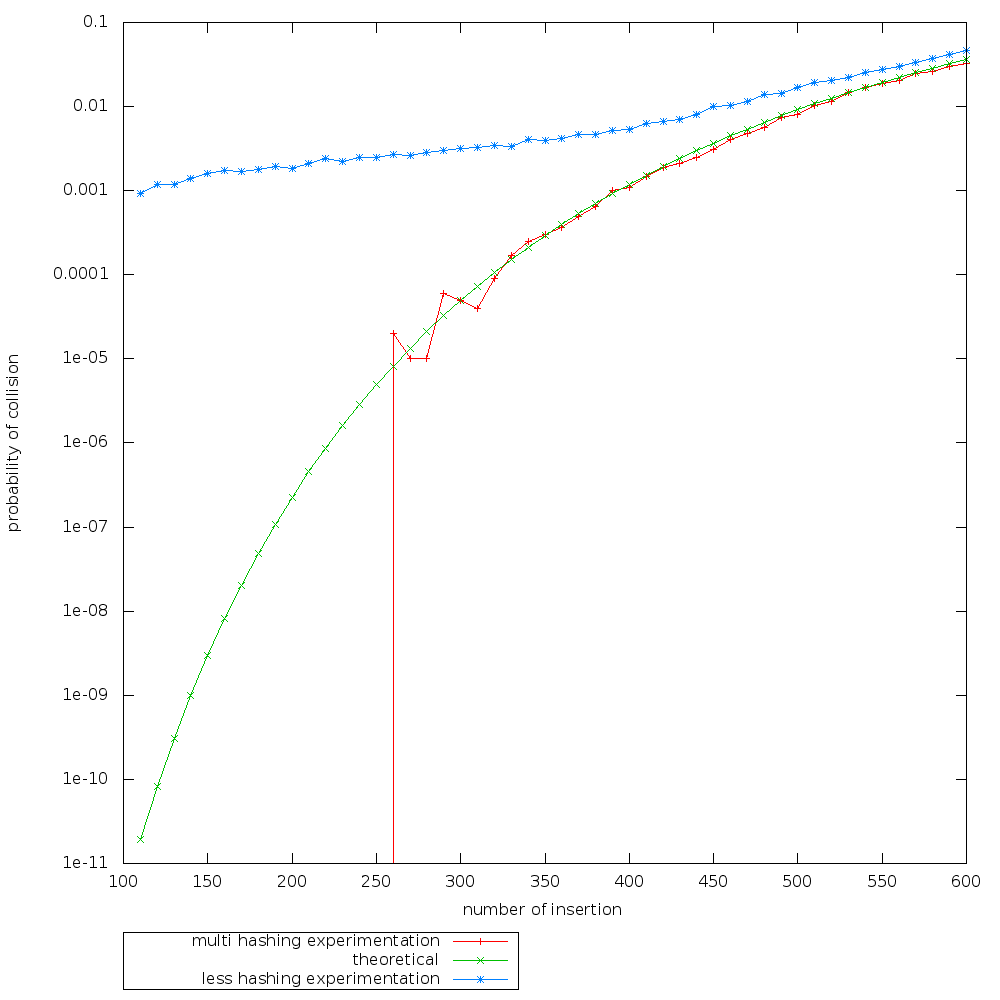
\includegraphics[width = 0.5\linewidth]{./image/bf/false_positive_probability.png}
 \caption{Testing the probability of getting a false positive with two different families of Hash functions} \label{fig:fpp}
\end{figure}
\paragraph{} The graphic above shows that the less hashing method, even if easy to compute, can not be used in our case because of the high probability of getting false positive. However this hashing method could be really interesting when hashing in a space of size $m$ growing linearly in the number of added element, because then it has the same asymptotic behaviour than an idependant hash family.(TODO : insert references) Such a growth of the size of the hashing space can not be used in our case where we suppose than we have no bound on the size of the history. Therefore we shall use the multiplication method which needs more computation but is more reliable, and the figure~\ref{fig:fpp} enables us to choose the number of element we can insert in a slice given a bound on the probability of false positive.
\section{Evaluation}
In this last part we will show some experimentations that have been done on the algorithm, mainly on the \texttt{explore} function.
\paragraph{} The exemple that is detailed for the algorithm used three slices in order to fully discover the difference. The number of slices needed to synchronize is important as it is the number of times the algorithm will be restarted on the server side and as it will be exchanged over the network. The following curves give the average number of slices needed to synchronize regarding the high of the dag and the $p$ factor (previously detailed)
 \begin{figure}[H]
 \centering
  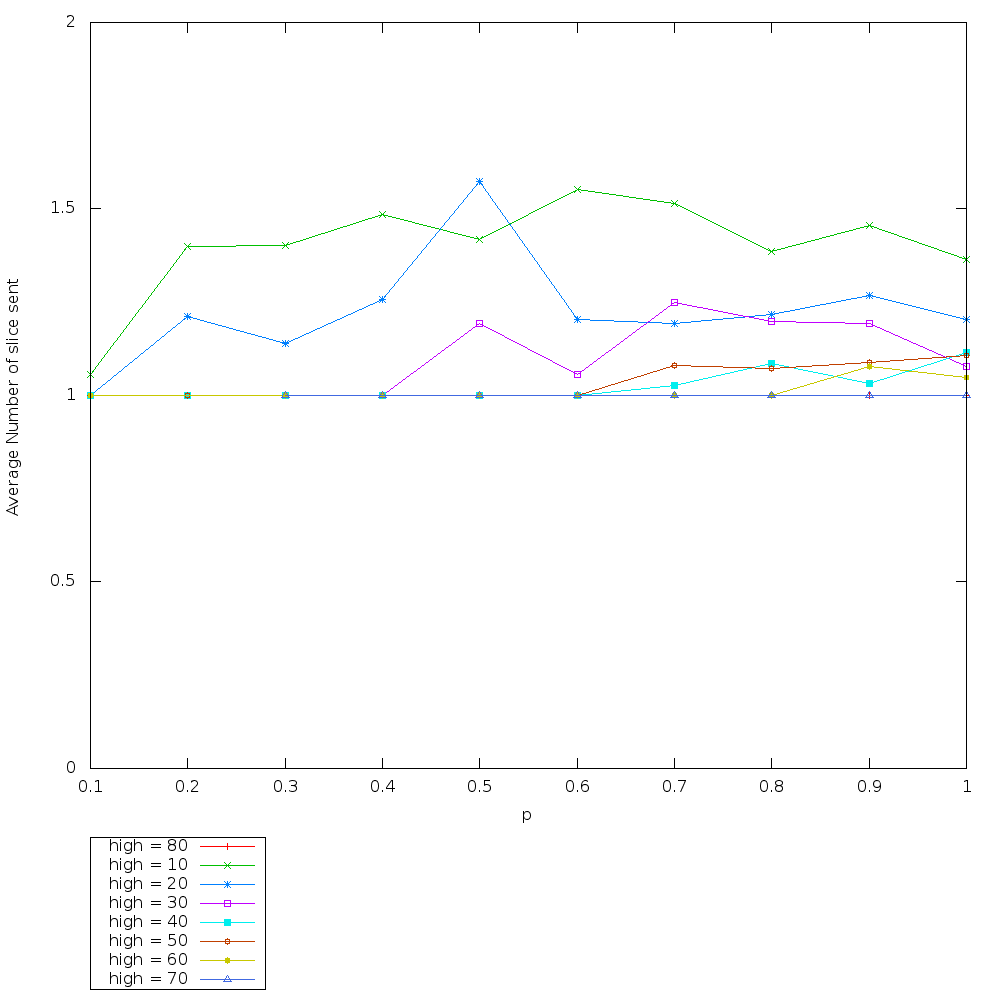
\includegraphics[height=10cm]{./image/slicesent/Nb_sent_slice.png}
  \caption{Graph of 1000 nodes with Slices of size 200}
 \end{figure}
 This graph underlines the fact that, whatever the shape of the DAG is, not a lot of slices are needed to synchronize. Therefore in this exemple the information sent by the client to synchronize fits in $20\times 320 \times 1.1 = 7040$ bits. $20$ is the number of hash functions we used, $320$ is the size of each table, and $1.1$ is the average number of slices.
 
 \paragraph{} The complexity of the explore algorithm is difficult to assert, given that it mainly depends on the shape of the tree. However we counted the number of call to the functions \texttt{pred} and \texttt{succ} of the \texttt{OcamlGraph} library as well as the number of visit to each nodes. We chose to count those calls because they are the one with the biggest complexity (according to the \texttt{OcamlGraph} documentation). The following curves shows the average values of this calls divided by the size of the difference between the DAGs depending on different values. Each DAG had $1000$ nodes labelled with $160$ bits hash.
\begin{figure}[H]
 \centering
  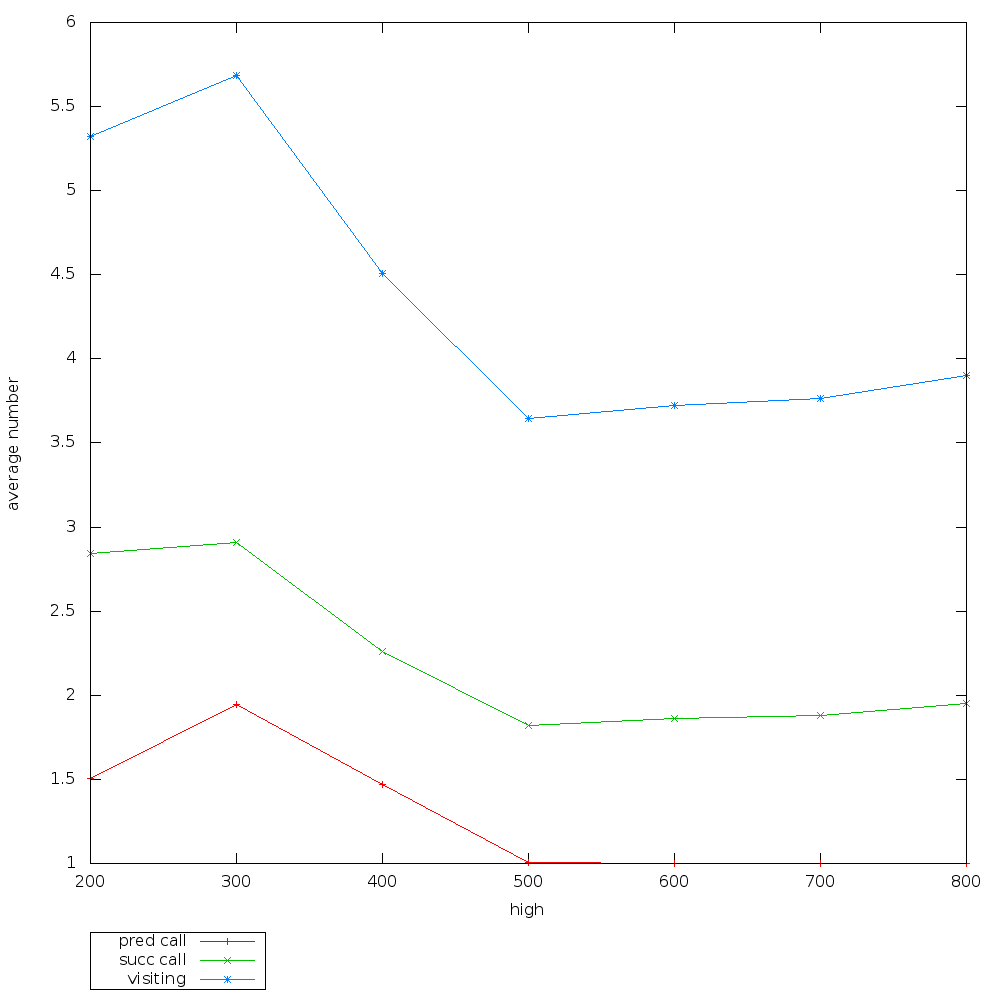
\includegraphics[height=10cm]{./image/eval/call_depending_on_high_over_size.png}
  \caption{Number of calls depending on the high of the DAG}
 \end{figure}
 \begin{figure}[H]
 \centering
  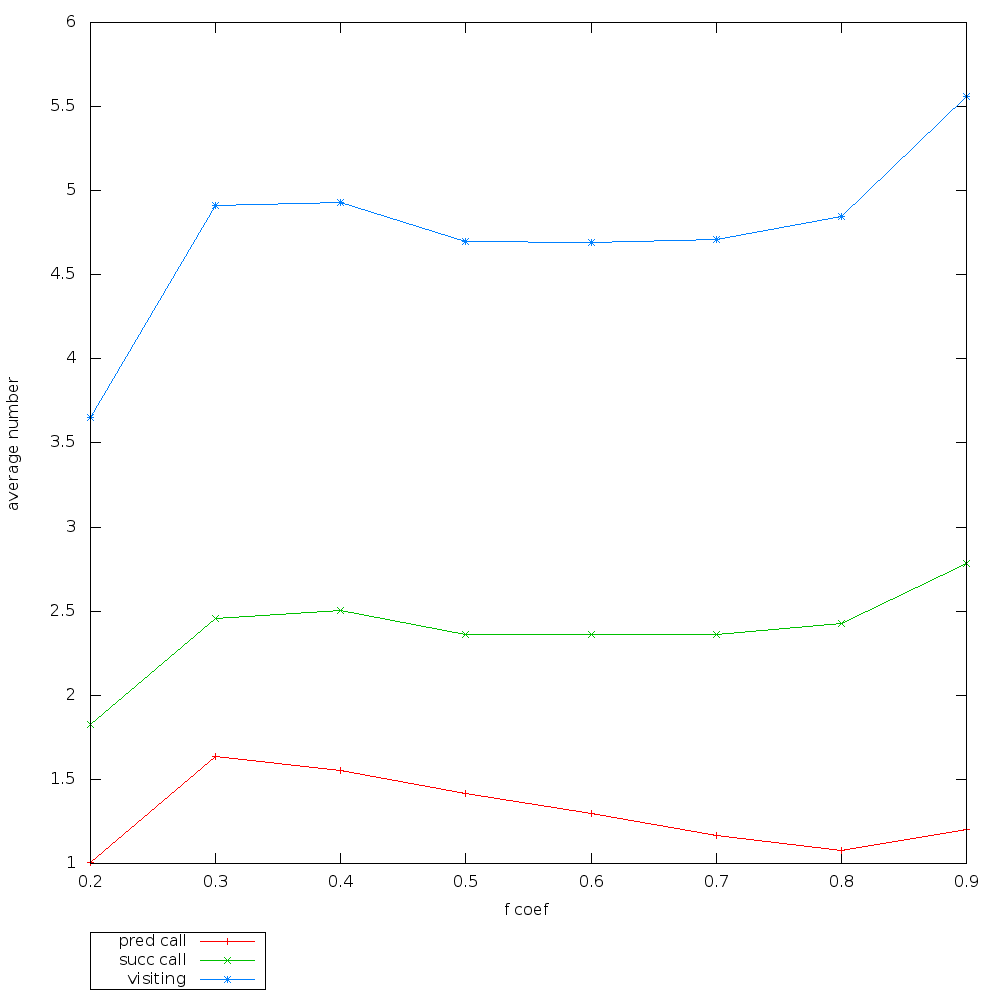
\includegraphics[height=10cm]{./image/eval/call_depending_on_f_coef.png}
  \caption{Number of calls depending on average number of predecessors}
 \end{figure}
 The two previous graphs underline that the complexity in terms of call to the \texttt{pred} and \texttt{succ} function is linear on the size of the difference between the two DAGs that are being synchronized, which is the main result we wanted. Indeed in the case where we want our algorithm to work it is important that the complexity does not increase with the size of the history but only with the size of the difference.
\chapter{Conclusion and bibliography}
%   \input{biblio.tex}
\chapter{Appendix}
\section{DAG Generator}
\label{sec:daggen}
I wrote the DAG generator that we used thanks to the OCamlgraph Librairy. The Dag Generator is a functor with signature :
\begin{lstlisting}
module type Elem = 
sig
  type t
  (** [init n] initializes the Random element generator where [n] is a seed
  *)
  val init : int -> unit
  (** [next_item n] gives back a new element where [n] is the size of the new element
  *)
  val next_item : int -> t
end
module Make :
  functor (B : Graph.Sig.I) ->
    functor (L : Elem with type t = B.V.t) ->
      sig
	(** [alea n h t seed p] is the function that produces a dag
	and the biggest element of this dag where [n] is the
	number of nodes of the dag and [h] is the high of the dag
	and [t] is the size of the element in the dag and [seed]
	is the seed used to initialize the element generator and
	[p] is the probability that a node of high i is the son of
	a node of high (i-1)
	*)
	val alea : int -> int -> int -> int -> float -> B.t * B.V.t
      end
\end{lstlisting}

\begin{figure}[H]
 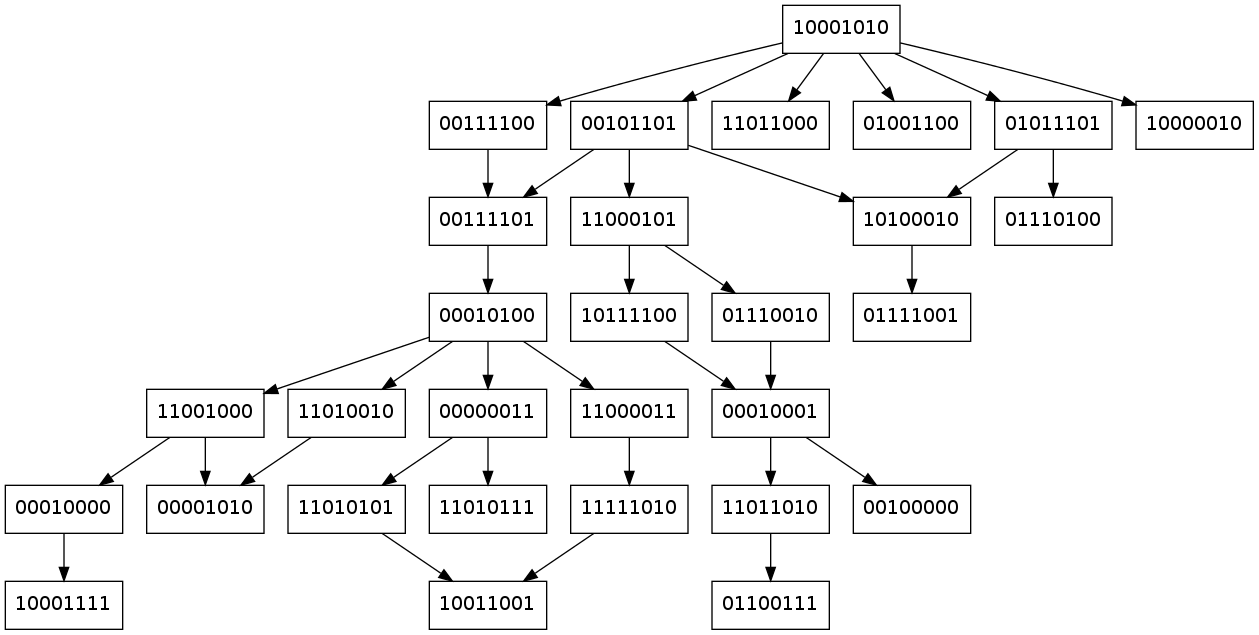
\includegraphics[width = \textwidth]{./image/DagGen/output025.png}
 \caption{DAG generated with $p=0.25$} \label{DAGgen}
\end{figure}
\begin{figure}[H]
 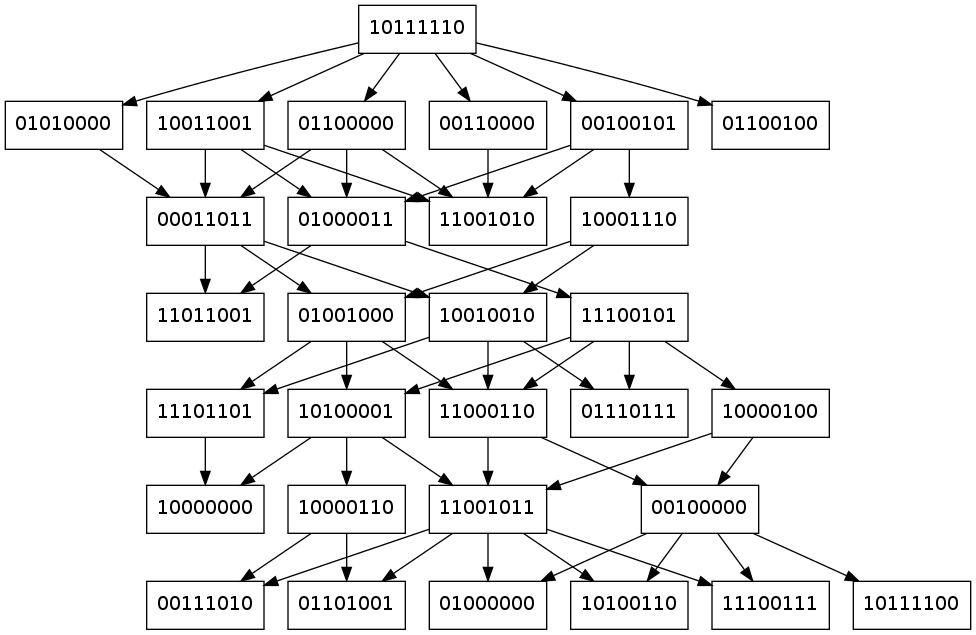
\includegraphics[width = \textwidth]{./image/DagGen/output05.png}
 \caption{DAG generated with $p=0.5$}
\end{figure}
\begin{figure}[H]
 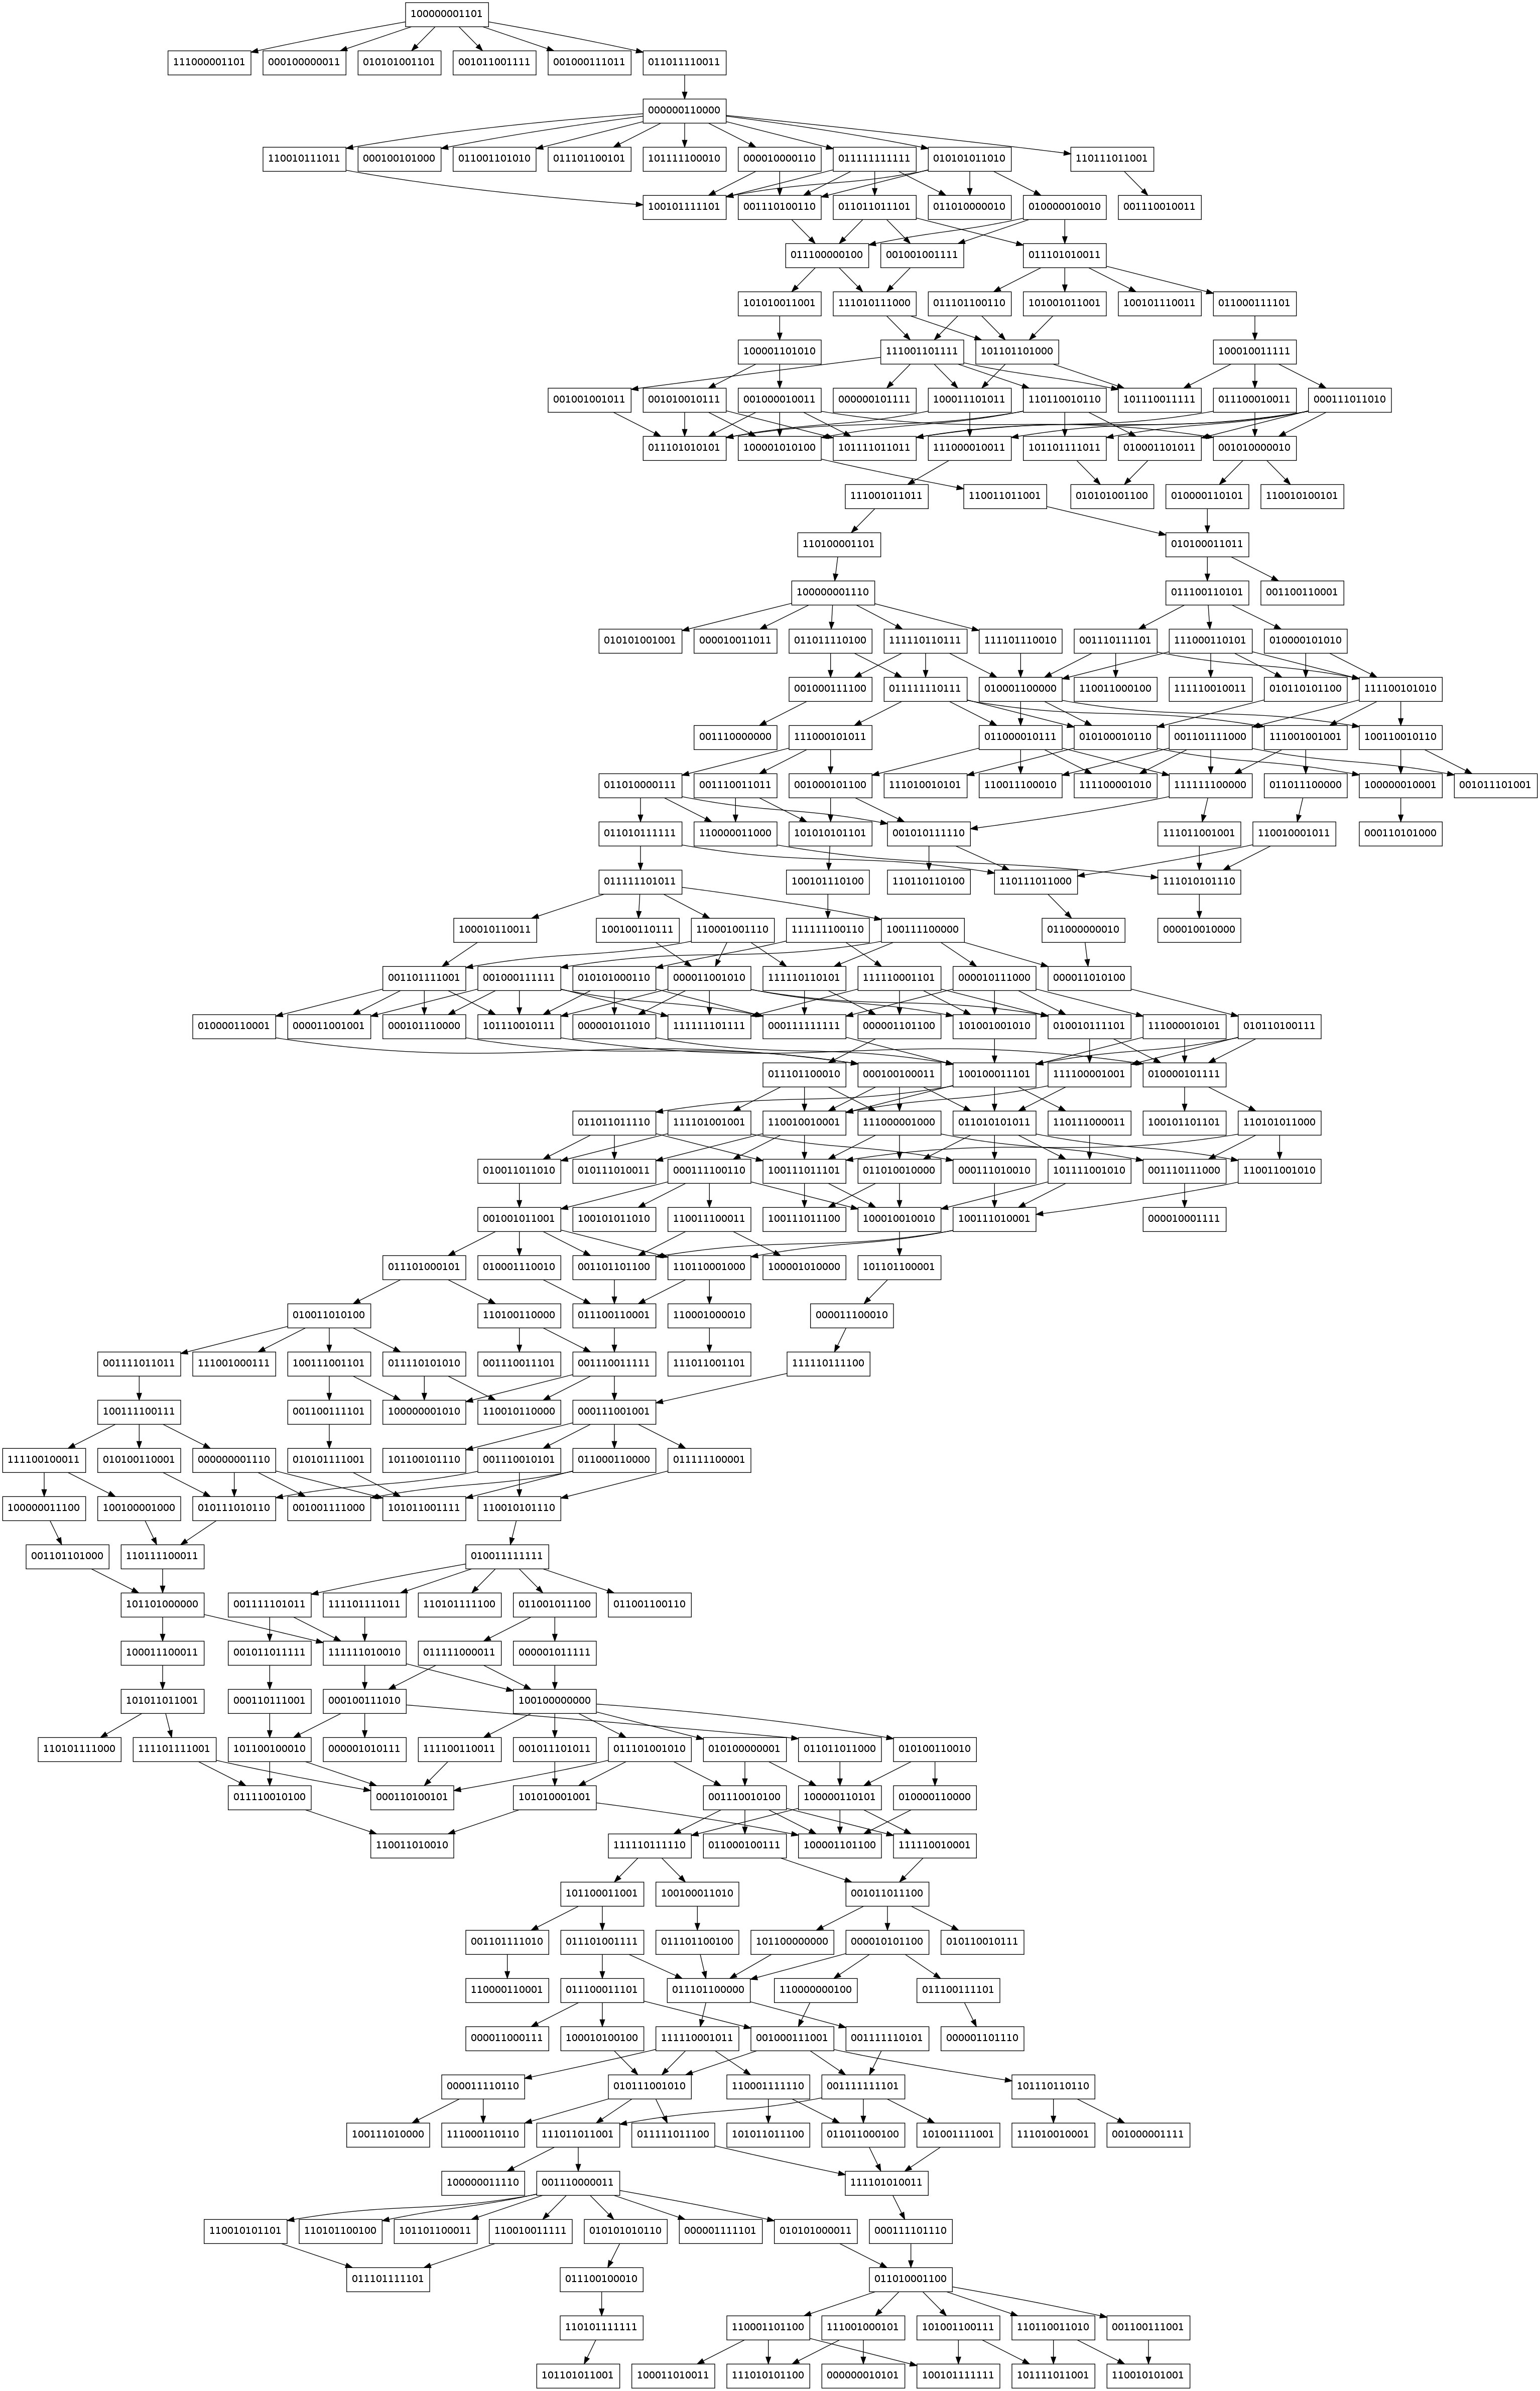
\includegraphics[width = \textwidth]{./image/DagGen/outputbig.png}
 \caption{A full git tree}
\end{figure}
\section{Detailed Algorithm}
\label{sec:detailedalgo}
 \begin{algorithm}[H]
  \SetAlgoLined
  \caption{Finding some of the ancestors of $Alice$ not known by $Bob$}
  \SetKwInOut{Input}{input}\SetKwInOut{Output}{output}
  \SetKwComment{tcc}{(*}{*)}
  \KwData{\texttt{Alice\_Heads} : some nodes in the history of $Alice$, \texttt{Ancestor} : a dag of the ancesters of $Alice$, \texttt{G\_In} : a graph of ancestors of $Alice$ not known by $Bob$, \texttt{Bf} : The Bloom filter of $Bob$, \texttt{Bd} : The Border of $Bob$}
%   \KwData{
%     \begin{itemize}
%     \item \texttt{Alice\_Heads} : some nodes in the history of $Alice$
%     \item \texttt{Ancestor} : a dag of the ancesters of $Alice$
%     \item \texttt{G\_In} : a graph of ancestors of $Alice$ not known by $Bob$
%     \item \texttt{Bf} : The Bloom filter of $Bob$
%     \item \texttt{Bd} : The Border of $Bob$
%     \end{itemize}
%     }
  \KwResult{\texttt{G\_Out} : a graph of ancestors of $Alice$ not known by $Bob$, \texttt{node\_to\_check} : a list of ancestors of $Alice$ that shall be revisited with the next Bloomfilters}
%   \KwResult{
%   \begin{itemize}
%   \item \texttt{G\_Out} : a graph of ancestors of $Alice$ not known by $Bob$
%   \item \texttt{node\_to\_check} : a list of ancestors of $Alice$ that shall be revisited with the next Bloomfilters
%   \end{itemize}
%   }
  
\SetAlgoLined\DontPrintSemicolon

  \texttt{explored} = $\varnothing$\;
  \texttt{in\_bf} = $\varnothing$\;
  \texttt{in\_border} = $\varnothing$\;
  \texttt{to\_further\_explore} = $\varnothing$\;
\SetKwFunction{explore}{\textbf{explore}}
\SetKwFunction{belong}{\textbf{belong}}
\SetKwFunction{addv}{\textbf{add\_vertex}}
\SetKwFunction{adde}{\textbf{add\_edge}}
\SetKwFunction{succ}{\textbf{successor}}
\SetKwFunction{pred}{\textbf{predecessor}}
\SetKwProg{myproc}{Procedure}{}{}
\myproc{\explore{\texttt{node}}}{

\If{\texttt{node} $\notin$ \texttt{explored}}
{
\texttt{explored} = \texttt{node} $\cup$ \texttt{explored}\;
\eIf{\belong{\texttt{node,\texttt{Bf}}}}{
  \texttt{in\_bf} = \texttt{node} $\cup$ \texttt{in\_bf}\;
  }
  {
  \eIf{\belong{\texttt{node,\texttt{Bd}}}}{
  \texttt{in\_border} = \texttt{node} $\cup$ \texttt{in\_border}\;
  }
  {
  \For{\texttt{pere} $\in$ \pred{\texttt{Ancestor},\texttt{node}}}{
    \explore{\texttt{pere}}
  }
  }
  }
}
}
\SetKwFunction{bf}{\textbf{find\_in\_bf}}
\SetKwFunction{bd}{\textbf{find\_in\_border}}
\myproc{\bf{\texttt{node}}}{
  \If{$\texttt{node} \notin \texttt{explored} \wedge \texttt{node} \notin \texttt{G\_In}$}{
    \addv{\texttt{G\_In},\texttt{node}}\;
    \For{\texttt{fils} $\in$ \succ{\texttt{Ancestor},\texttt{node}}}{
      \adde{\texttt{G\_In},\texttt{node},\texttt{fils}}\;
      \bf{\texttt{fils}}
    }
  }
}
\myproc{\bd{\texttt{node}}}{
  \If{$\texttt{node} \notin \texttt{explored}$}{
    \eIf{$\texttt{node} \in \texttt{G\_In}$}{
      \texttt{to\_further\_explore} = \texttt{node} $\cup$ \texttt{to\_further\_explore}\;
    }
    {
      \For{\texttt{fils} $\in$ \succ{\texttt{Ancestor},\texttt{node}}}{
      \bd{\texttt{fils}}
      }    
    }
  }
}
\For{\texttt{node} $\in$ \texttt{Alice\_Heads}}{
  \explore{\texttt{node}}
}
\texttt{explored} = $\varnothing$\;
\For{\texttt{node} $\in$ \texttt{in\_bf}}{
  \bf{\texttt{node}}
}
\texttt{explored} = $\varnothing$\;
\For{\texttt{node} $\in$ \texttt{in\_border}}{
  \bd{\texttt{node}}
}
\KwRet{(\texttt{G\_In,to\_further\_explore})}

  \end{algorithm}
  
\section{Signatures}
\label{sec:datasig}
\begin{lstlisting}
module type DataSig =
  sig
  (** type t is the type of the data we are trying to store *)
  type t
  (** type u is the type of the storage that are used *)
  type u
  val nb_max : int
  (** [merge lu lt] is a function that computes the union of storages
      and add some new data where [lu] is the storages we want to unite
      and [lt] the data we want to add *)
  val merge : u list -> t list -> u
  (** [mem e s] tests the membership where [e] is the data and [s] is
      the storage *)
  val mem : t -> u -> bool
end
\end{lstlisting}
%   In the following we will consider two DAGs, each with some particular nodes called head. The set of heads is the smallest set so that every node in the considered DAG is an ancestor of one of the head. One of the DAG will be refered to as Client or $Bob$ and the other one as Server or $Alice$. $\mathrm{Ancestor}(Alice)$ and $\mathrm{Ancestor}(Bob)$ are the considered DAGs and the aim of the algorithm is to be able to compute $\mathrm{Ancestor}(Alice) \setminus \mathrm{Ancestor}(Bob) = \{ x\ ,\ x \in \mathrm{Ancestor}(Alice) \wedge x \notin \mathrm{Ancestor}(Bob)\}$. The complexity of the algorithm will be expressed in terms of $n = \#(\mathrm{Ancestor}(Alice) \setminus \mathrm{Ancestor}(Bob))$. In terms of application, the client and the server are two entities that are physically distinct, therefore it was important during the design of the algorithm to keep in mind and to be aware that :
\begin{enumerate}
 \item The quantity of information exchanged between the two processes shall be the smaller possible
 \item We want to minimise the complexity on both processes
 \item There can be no no pre-assumptions on the shape of the graph, because the shape of the global DAG (with multiple head) is evolving in time and is not known at the beginning.
 \item There is no high authority that has a memory of every thing.
\end{enumerate}
\paragraph{} The section~\ref{sec:prelim} underlined that we were not able to find a way to compute easily the set of BCA, moreover if the server has to send the difference $\mathrm{Ancestor}(Alice) \setminus \mathrm{Ancestor}(Bob)$ then at some point we will have to go all over this difference, therefore we decided that the server could cross the part of its history corresponding to the difference.
% However the server does not know what nodes are already in the history of the client. Hence the client need to send to the server its history so that the server knows when the exploration of its past shal stop. Sending all of the client's history can requiere a huge exchange of data, moreover in applications we are interested in (git) the difference we are trying to compute is usually small compared to the size of the all history. the client shall therefore only send the latest event in its history (a fixed number) so that in most case the server manages to make the link between the two histories. However 
% in some cases the server will not be able to find any of the client's latest node in its history, in such cases the server will have to go throw all of its history (because the link can be anywhere) to understand that it has nothing in common with this set of latest nodes. We do not want the server to go throw all of its history as we have no bound on the size of this history. Thus the client need to tell the server that at some point of its exploration the server need to stop because there is no point in continuing the exploration. We introduce the Border of a set of nodes $A$ as defined such that for every nodes in $A$ each of its predecessor are either in $A$ or in the border of $A$. To sum up, the client divides its history in packages that will be called "window" and to each window we associate a "border" (see \ref{fig:twoproc}). Now if the client send a window and the union of all the borders to the server, this one will, at some point, find one of the two while exploring its history bottom-up and 
% therefore will not have to go across all of its history.
\begin{definition}
 Given a DAG $\mathcal{D}$ and a partition of a the nodes of $\mathcal{D}$, we call a set of equivalent nodes for this partition a "slice of $\mathcal{D}$"
\end{definition}
\begin{definition}
 Given a DAG $\mathcal{D}$ and a slice $\mathcal{S}$ we call the border of $\mathcal{S}$ (noted $\overline{\mathcal S}$)the smallest set such that $\forall x \in \mathcal{D},\ \forall y\in \mathrm{predecessor}{x} y\in \mathcal{S} \vee y \in \overline{\mathcal S}$.
\end{definition}
\paragraph{Idea of the algorithm} We assume that a partition of its DAG of ancestors is known by the client as well as well as a border for every slice of the partition.
\begin{enumerate}
 \item The client sends the list of its head, one of its slice and the union of all the border to the Server
 \item The server goes up in its history and stop whenever it crosses a node in the slice are in the border.
 \item The server computes the DAG $D$ of the successors of every nodes it found in slice.
 \item The server computes a list of "nodes of interest" from which it shall starts again the exploration (those "nodes of interest" are the last successors of the nodes found in the border that are not in $D$)
 \item The server sends back $D$ and the list of "nodes of interest"
 \item The client starts again with anoter slice and instead of the list of its head it sends the list of "nodes of interest" it received from the server, except if there is no "node of interest" in which case the algorithm stop.
\end{enumerate}
\paragraph{} This algorithm as the property that the server have absolutely no memory. The figure~\ref{fig:twoproc} shows a partition of two dags in slices.

\begin{figure}[H]
\centering
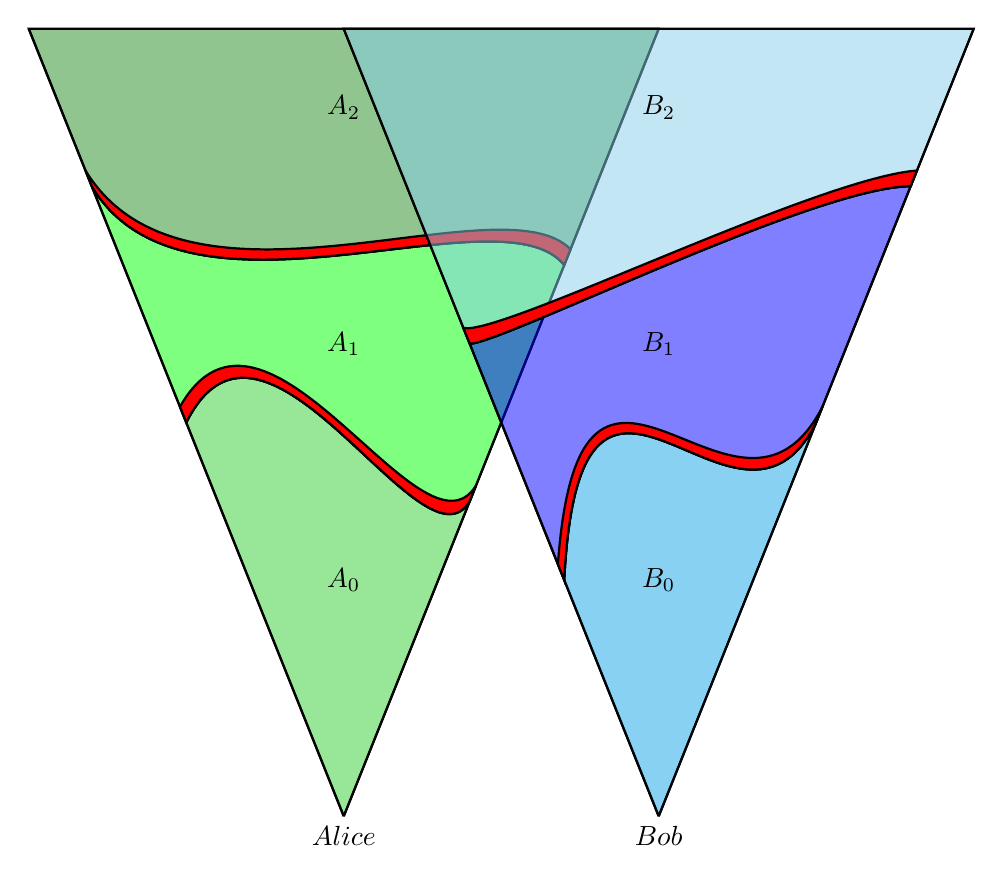
\begin{tikzpicture}
\begin{scope}
\coordinate[label=below:$Alice$] (A) at (0,0) ;
\coordinate (B) at (4,10);
\coordinate (C) at (-4,10);
\draw [thick] (A) -- (B) coordinate[pos = 0.4] (B1) {} coordinate [pos = 0.42] (B1b) {} coordinate[pos = 0.7] (B2) {} coordinate[pos = 0.72] (B2b) {};
\draw [thick] (B) -- (C) coordinate[pos = 0.5] (midBC) {};
\draw [thick] (A) -- (C) coordinate[pos = 0.5] (C1) {} coordinate [pos = 0.52] (C1b) {} coordinate[pos = 0.8] (C2) {} coordinate[pos = 0.82] (C2b) {};
\draw [thick, fill = LimeGreen,fill opacity = 0.5] (A) -- (B1) .. controls (1,3) and (-1,7) .. (C1) -- (A);
\draw [thick, fill = green,fill opacity = 0.5] (B1) .. controls (1,3) and (-1,7) .. (C1) -- (C2) .. controls (-2,6) and (2,8) .. (B2) -- (B1);
\draw [thick, fill = ForestGreen, fill opacity = 0.5] (C2) .. controls (-2,6) and (2,8) .. (B2) -- (B) -- (C) -- (C2);
\draw [thick, fill = red, fill opacity = 1] (B1b) .. controls (1,3.1) and (-1,7.1) .. (C1b) -- (C1) .. controls (-1,7) and (1,3) .. (B1) -- (B1b);
\draw [thick, fill = red, fill opacity = 1] (C2) .. controls (-2,6) and (2,8) .. (B2) -- (B2b) .. controls (2,8.1) and (-2,6.1) .. (C2b) -- (C2);
\draw [draw = none] (A) -- (midBC) node[pos = 0.3] {$A_0$} node[pos = 0.6] {$A_1$} node[pos = 0.9] {$A_2$};

\end{scope}
\begin{scope}[shift={(4cm,0cm)}]
\coordinate[label=below:$Bob$] (D) at (0,0);
\coordinate (E) at (4,10);
\coordinate (F) at (-4,10);
\draw [thick] (D) -- (E) coordinate[pos = 0.5] (E1) {} coordinate [pos = 0.52] (E1b) {} coordinate[pos = 0.8] (E2) {} coordinate[pos = 0.82] (E2b) {};
\draw [thick] (E) -- (F) coordinate[pos = 0.5] (midEF) {};
\draw [thick] (D) -- (F) coordinate[pos = 0.3] (F1) {} coordinate [pos = 0.32] (F1b) {} coordinate[pos = 0.6] (F2) {} coordinate[pos = 0.62] (F2b) {};
\draw [thick, fill = Cerulean,fill opacity = 0.5] (D) -- (E1) .. controls (1,3) and (-1,7) .. (F1) -- (D);
\draw [thick, fill = blue,fill opacity = 0.5] (E1) .. controls (1,3) and (-1,7) .. (F1) -- (F2) .. controls (-2,6) and (2,8) .. (E2) -- (E1);
\draw [thick, fill = SkyBlue, fill opacity = 0.5] (F2) .. controls (-2,6) and (2,8) .. (E2) -- (E) -- (F) -- (F2);
\draw [thick, fill = red, fill opacity = 1] (E1b) .. controls (1,3.1) and (-1,7.1) .. (F1b) -- (F1) .. controls (-1,7) and (1,3) .. (E1) -- (E1b);
\draw [thick, fill = red, fill opacity = 1] (F2) .. controls (-2,6) and (2,8) .. (E2) -- (E2b) .. controls (2,8.1) and (-2,6.1) .. (F2b) -- (F2);
\draw [draw = none] (D) -- (midEF) node[pos = 0.3] {$B_0$} node[pos = 0.6] {$B_1$} node[pos = 0.9] {$B_2$};
\end{scope}
\end{tikzpicture}
\caption{Two processes sharing a part of their history and their decomposition in Slices and Borders} \label{fig:twoproc}
\end{figure}
The figure~\ref{fig:twoproc} underlines the fact that it is interesting to have a interesting partition of the node, in the sense that :
\begin{enumerate}
 \item We want the borders to be small so that we do not have to send a lot of information
 \item We want to do the least sending/receiving data to/from the server possible
 \item We want those slices/border to be easy to compute, in the sense that we do not want to cross all of the history of the client each time we want to merge
 \item We want the slices to be all of the same size
\end{enumerate}
Let us assume we decided that the slices should be of size $n$ and that a process already knows a partition $\mathcal{P} = \{A_0,\cdots,A_m\}$ in slices of its ancestors and the paired borders. This process needs to add some nodes $S$ in its history. We start by filling the set in the partition with a size smaller that $n$, by adding the element from $S$ in an order verifying the order of the DAG. Therefore if $S$ contains two nodes $a$ and $b$, $a$ being a predecessor of $b$ then $a$ will be added prior than $b$. Once every partition is of size $n$ we add a new slice to $\mathcal P$. While adding a node in one of the slices we add it in the border if one of its parents is not in the slice. The order in which we add the elements ensures us that the border will be the small (regarding the number of element in the slice). Hence we can build a new partition and the corresponding borders quite easily from the previous one. Finally in order to ensure that there is not a lot of exchanges between the client and the server, the client send its slices from the newest to the oldest one. For example in figure~\ref{fig:twoproc} Bob will be sending the slices in the order $B_0$ then $B_1$ then $B_2$.
\begin{algorithm}[H] 
  \SetAlgoLined
  \caption{Finding some of the ancestors of $Alice$ not known by $Bob$}
  \SetKwInOut{Input}{input}\SetKwInOut{Output}{output}
  \SetKwComment{tcc}{(*}{*)}
  \KwData{\texttt{Alice\_Heads} : some nodes in the history of $Alice$, \texttt{Ancestor} : a dag of the ancesters of $Alice$, \texttt{G\_In} : a graph of ancestors of $Alice$ not known by $Bob$, \texttt{Bf} : The Bloom filter of $Bob$, \texttt{Bd} : The Border of $Bob$}
%   \KwData{
%     \begin{itemize}
%     \item \texttt{Alice\_Heads} : some nodes in the history of $Alice$
%     \item \texttt{Ancestor} : a dag of the ancesters of $Alice$
%     \item \texttt{G\_In} : a graph of ancestors of $Alice$ not known by $Bob$
%     \item \texttt{Bf} : The Bloom filter of $Bob$
%     \item \texttt{Bd} : The Border of $Bob$
%     \end{itemize}
%     }
  \KwResult{\texttt{G\_Out} : a graph of ancestors of $Alice$ not known by $Bob$, \texttt{node\_to\_check} : a list of ancestors of $Alice$ that shall be revisited with the next Bloomfilters}
%   \KwResult{
%   \begin{itemize}
%   \item \texttt{G\_Out} : a graph of ancestors of $Alice$ not known by $Bob$
%   \item \texttt{node\_to\_check} : a list of ancestors of $Alice$ that shall be revisited with the next Bloomfilters
%   \end{itemize}
%   }
  
\SetAlgoLined\DontPrintSemicolon
\SetKwFunction{explore}{\textbf{explore}}
\SetKwFunction{belong}{\textbf{belong}}
\SetKwFunction{addv}{\textbf{add\_vertex}}
\SetKwFunction{adde}{\textbf{add\_edge}}
\SetKwFunction{succ}{\textbf{successor}}
\SetKwFunction{pred}{\textbf{predecessor}}
\SetKwProg{myproc}{Procedure}{}{}
\myproc{\explore{\texttt{node},\texttt{visited},\texttt{in\_bf},\texttt{in\_border}}}{

  \eIf{\belong{\texttt{node,\texttt{Bf}}}}{
    \KwRet{(\texttt{visited} $\cup$ \texttt{node},\texttt{in\_bf} $\cup$ \texttt{node},\texttt{in\_border})}
  }
  {
    \eIf{\belong{\texttt{node,\texttt{Bd}}}}{
    \KwRet{(\texttt{visited} $\cup$ \texttt{node},\texttt{in\_bf} ,\texttt{in\_border}$\cup$ \texttt{node})}
    }
    {
      \texttt{visited\_already} = \texttt{node} $\cup$ \texttt{visited}\;
      \texttt{in\_bf\_already} = \texttt{in\_bf}\;				
      \texttt{in\_border\_already} = \texttt{in\_border}\;
      \For{\texttt{pere} $\in$ \pred{\texttt{Ancestor},\texttt{node}}}{
      \If{\texttt{pere} $\notin$ \texttt{explored}}
      {
	\texttt{visited\_already,in\_bf\_already,in\_border\_already} = \explore{\texttt{pere},\texttt{visited\_already},\texttt{in\_bf\_already},\texttt{in\_border\_already}}\;
      }
      }
      \KwRet{(\texttt{visited\_already},\texttt{in\_bf\_already},\texttt{in\_border\_already})}\;
    }	
  }
}

\SetKwFunction{bf}{\textbf{find\_in\_bf}}
\SetKwFunction{bd}{\textbf{find\_in\_border}}
\myproc{\bf{\texttt{node},\texttt{explored}}}{
    \addv{\texttt{G\_In},\texttt{node}}\;
    \texttt{already\_explored} = \texttt{explored} $\cup$ \texttt{node}\;
    \For{\texttt{fils} $\in$ \succ{\texttt{Ancestor},\texttt{node}}}{
      \adde{\texttt{G\_In},\texttt{node},\texttt{fils}}\;
      \If{$\texttt{fils} \notin \texttt{already\_explored} \wedge \texttt{fils} \notin \texttt{G\_In}$}{
	\texttt{already\_explored} = \bf{\texttt{fils},\texttt{already\_explored}}
	}
    }
    \KwRet{already\_explored}
}

\myproc{\bd{\texttt{node},\texttt{explored},\texttt{to\_further\_explore}}}{
  \If{$\texttt{node} \notin \texttt{explored}$}{
    \texttt{son\_in} = $\varnothing$\;
    \texttt{son\_out} = $\varnothing$\;
    \For{\texttt{fils} $\in$ \succ{\texttt{Ancestor},\texttt{node}}}{
      \eIf{\texttt{fils} $\in$ \texttt{G\_In}}{
	\texttt{son\_in} = \texttt{fils} $\cup$ \texttt{son\_in}\; 
      }{
	\texttt{son\_out} = \texttt{fils} $\cup$ \texttt{son\_out}\;
      }
    }
    \texttt{already\_explored} = \texttt{explored}\;
    \texttt{inter\_node} = \texttt{to\_further\_explore}\;
    \If{\texttt{son\_in} = $\varnothing$}{
      \texttt{inter\_node} = \texttt{node} $\cup$ \texttt{inter\_node}\;
    }
    \For{\texttt{fils} $\in$ \texttt{son\_out}}{
      \If{\texttt{fils} $\notin$ \texttt{already\_explored}}{
	\texttt{already\_explored},\texttt{inter\_node} = \bd{\texttt{fils},\texttt{already\_explored},\texttt{inter\_node}}\;
      }
    }
    \KwRet{(already\_explored,inter\_node)}\;
  }
}
\end{algorithm}
  \begin{algorithm}
  \SetAlgoLined
  \caption{Finding some of the ancestors of $Alice$ not known by $Bob$}
  \SetKwInOut{Input}{input}\SetKwInOut{Output}{output}
  \SetKwComment{tcc}{(*}{*)}
  \KwData{\texttt{Alice\_Heads} : some nodes in the history of $Alice$, \texttt{Ancestor} : a dag of the ancesters of $Alice$, \texttt{G\_In} : a graph of ancestors of $Alice$ not known by $Bob$, \texttt{Bf} : The Bloom filter of $Bob$, \texttt{Bd} : The Border of $Bob$}
%   \KwData{
%     \begin{itemize}
%     \item \texttt{Alice\_Heads} : some nodes in the history of $Alice$
%     \item \texttt{Ancestor} : a dag of the ancesters of $Alice$
%     \item \texttt{G\_In} : a graph of ancestors of $Alice$ not known by $Bob$
%     \item \texttt{Bf} : The Bloom filter of $Bob$
%     \item \texttt{Bd} : The Border of $Bob$
%     \end{itemize}
%     }
  \KwResult{\texttt{G\_Out} : a graph of ancestors of $Alice$ not known by $Bob$, \texttt{node\_to\_check} : a list of ancestors of $Alice$ that shall be revisited with the next Bloomfilters}
%   \KwResult{
%   \begin{itemize}
%   \item \texttt{G\_Out} : a graph of ancestors of $Alice$ not known by $Bob$
%   \item \texttt{node\_to\_check} : a list of ancestors of $Alice$ that shall be revisited with the next Bloomfilters
%   \end{itemize}
%   }
  
\SetAlgoLined\DontPrintSemicolon

  \texttt{explored} = $\varnothing$\;
  \texttt{in\_bf} = $\varnothing$\;
  \texttt{in\_border} = $\varnothing$\;
  \texttt{to\_further\_explore} = $\varnothing$\;
\SetKwFunction{explore}{\textbf{explore}}
\SetKwFunction{belong}{\textbf{belong}}
\SetKwFunction{addv}{\textbf{add\_vertex}}
\SetKwFunction{adde}{\textbf{add\_edge}}
\SetKwFunction{succ}{\textbf{successor}}
\SetKwFunction{pred}{\textbf{predecessor}}
\SetKwProg{myproc}{Procedure}{}{}
\myproc{\explore{\texttt{node}}}{

\If{\texttt{node} $\notin$ \texttt{explored}}
{
\texttt{explored} = \texttt{node} $\cup$ \texttt{explored}\;
\eIf{\belong{\texttt{node,\texttt{Bf}}}}{
  \texttt{in\_bf} = \texttt{node} $\cup$ \texttt{in\_bf}\;
  }
  {
  \eIf{\belong{\texttt{node,\texttt{Bd}}}}{
  \texttt{in\_border} = \texttt{node} $\cup$ \texttt{in\_border}\;
  }
  {
  \For{\texttt{pere} $\in$ \pred{\texttt{Ancestor},\texttt{node}}}{
    \explore{\texttt{pere}}
  }
  }
  }
}
}
\SetKwFunction{bf}{\textbf{find\_in\_bf}}
\SetKwFunction{bd}{\textbf{find\_in\_border}}
\myproc{\bf{\texttt{node}}}{
  \If{$\texttt{node} \notin \texttt{explored} \wedge \texttt{node} \notin \texttt{G\_In}$}{
    \addv{\texttt{G\_In},\texttt{node}}\;
    \For{\texttt{fils} $\in$ \succ{\texttt{Ancestor},\texttt{node}}}{
      \adde{\texttt{G\_In},\texttt{node},\texttt{fils}}\;
      \bf{\texttt{fils}}
    }
  }
}
\myproc{\bd{\texttt{node}}}{
  \If{$\texttt{node} \notin \texttt{explored}$}{
    \eIf{$\texttt{node} \in \texttt{G\_In}$}{
      \texttt{to\_further\_explore} = \texttt{node} $\cup$ \texttt{to\_further\_explore}\;
    }
    {
      \For{\texttt{fils} $\in$ \succ{\texttt{Ancestor},\texttt{node}}}{
      \bd{\texttt{fils}}
      }    
    }
  }
}
\For{\texttt{node} $\in$ \texttt{Alice\_Heads}}{
  \explore{\texttt{node}}
}
\texttt{explored} = $\varnothing$\;
\For{\texttt{node} $\in$ \texttt{in\_bf}}{
  \bf{\texttt{node}}
}
\texttt{explored} = $\varnothing$\;
\For{\texttt{node} $\in$ \texttt{in\_border}}{
  \bd{\texttt{node}}
}
\KwRet{(\texttt{G\_In,to\_further\_explore})}
  
  \end{algorithm}
  
  \begin{figure}[H]
  \begin{minipage}{0.3\textwidth}
  \centering
  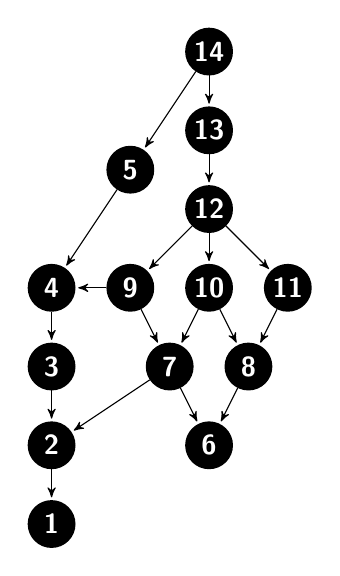
\begin{tikzpicture}[->,>=stealth',shorten >=1pt,auto,node distance=3cm,
  thick,main node/.style={circle,fill=blue!20,draw,font=\sffamily\Large\bfseries}]
  
  \foreach \place/\x in {{(0,0)/1}, {(0,1)/2},{(0,2)/3},{(0,3)/4}, {(1,4.5)/5}, {(2,1)/6}, {(1.5,2)/7},{(2.5,2)/8},{(1,3)/9},{(2,3)/10},{(3,3)/11},{(2,4)/12},{(2,5)/13},{(2,6)/14}}
  \node[arn_n] (a\x) at \place {\x};
%   Alice history
  \path[thin] (a14) edge (a5);
  \path[thin] (a5) edge (a4);
  \path[thin] (a4) edge (a3);
  \path[thin] (a3) edge (a2);
  \path[thin] (a2) edge (a1);
  \path[thin] (a9) edge (a4);
  \path[thin] (a7) edge (a2);
%   both history
  \path[thin] (a14) edge (a13);
  \path[thin] (a13) edge (a12);
  \path[thin] (a12) edge (a9);
  \path[thin] (a12) edge (a10);
  
  \path[thin] (a9) edge (a7);
  \path[thin] (a10) edge (a7);
%   Bob history
  \path[thin] (a12) edge (a11);
  \path[thin] (a11) edge (a8);
  \path[thin] (a10) edge (a8);
  \path[thin] (a7) edge (a6);
  \path[thin] (a8) edge (a6);
  \end{tikzpicture}
  \caption{Main Graph}
  \end{minipage}%
  \begin{minipage}{0.3\textwidth}
  \centering
  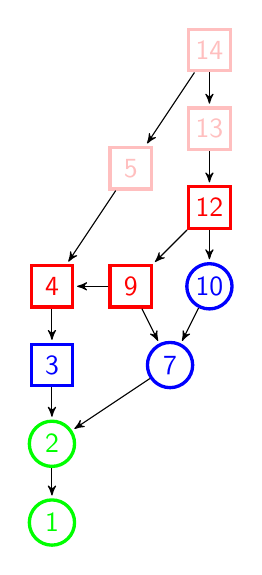
\begin{tikzpicture}[->,>=stealth',shorten >=1pt,auto,node distance=3cm,
  thick,main node/.style={circle,fill=blue!20,draw,font=\sffamily\Large\bfseries}]
  \foreach \place/\x in {{(0,0)/1}, {(0,1)/2}}
  \node[arn_g] (a\x) at \place {\x};
  
  
  \node[arn_pis] (a5) at (1,4.5) {5};
  \node[arn_pis] (a13) at (2,5) {13};
  \node[arn_pis] (a14) at (2,6) {14};
  
  
  \node[arn_b] (a10) at (2,3) {10};
  \node[arn_b] (a7) at (1.5,2) {7};
  \node[arn_bs] (a3) at (0,2) {3};
  
  \node[arn_rs] (a9) at (1,3) {9};
  \node[arn_rs] (a12) at (2,4) {12};
  \node[arn_rs] (a4) at (0,3) {4};
  %   Alice history
  \path[thin] (a14) edge (a5);
  \path[thin] (a5) edge (a4);
  \path[thin] (a4) edge (a3);
  \path[thin] (a3) edge (a2);
  \path[thin] (a2) edge (a1);
  \path[thin] (a9) edge (a4);
  \path[thin] (a7) edge (a2);
%   both history
  \path[thin] (a14) edge (a13);
  \path[thin] (a13) edge (a12);
  \path[thin] (a12) edge (a9);
  \path[thin] (a12) edge (a10);
  
  \path[thin] (a9) edge (a7);
  \path[thin] (a10) edge (a7);
  \end{tikzpicture}
  \caption{Alice's ancestors}
\end{minipage}%
\begin{minipage}{0.3\textwidth}
\centering
  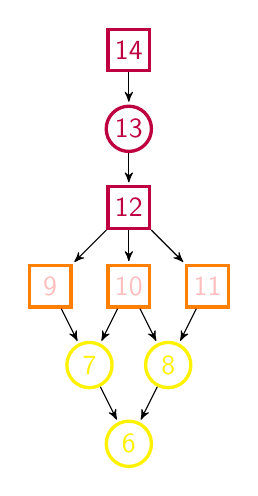
\begin{tikzpicture}[->,>=stealth',shorten >=1pt,auto,node distance=3cm,
  thick,main node/.style={circle,fill=blue!20,draw,font=\sffamily\Large\bfseries}]
%   
  \node[arn_y] (a6) at (2,1) {6};
  \node[arn_y] (a7) at (1.5,2) {7};
  \node[arn_y] (a8) at (2.5,2) {8};
  \node[arn_ts] (a9) at (1,3) {9};
  \node[arn_ts] (a10) at (2,3) {10};
  \node[arn_ts] (a11) at (3,3) {11};
  \node[arn_pus] (a12) at (2,4) {12};
  \node[arn_pu] (a13) at (2,5) {13};
  \node[arn_pus] (a14) at (2,6) {14};
  
%   both history
  \path[thin] (a14) edge (a13);
  \path[thin] (a13) edge (a12);
  \path[thin] (a12) edge (a9);
  \path[thin] (a12) edge (a10);
  
  \path[thin] (a9) edge (a7);
  \path[thin] (a10) edge (a7);
%   Bob history
  \path[thin] (a12) edge (a11);
  \path[thin] (a11) edge (a8);
  \path[thin] (a10) edge (a8);
  \path[thin] (a7) edge (a6);
  \path[thin] (a8) edge (a6);
  \end{tikzpicture}
  \caption{Bob's ancestors}

\end{minipage}
\end{figure}

\begin{figure}[H]
\begin{minipage}{0.3\textwidth}
\centering
 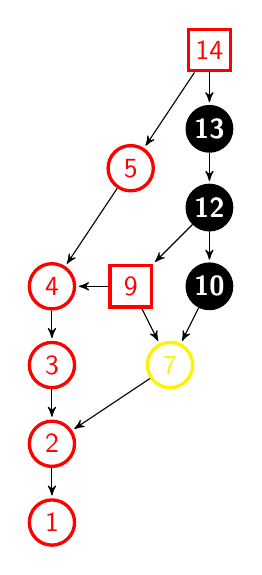
\begin{tikzpicture}[->,>=stealth',shorten >=1pt,auto,node distance=3cm,
  thick,main node/.style={circle,fill=blue!20,draw,font=\sffamily\Large\bfseries}]
  
  
  
  \node[arn_r] (a1) at (0,0) {1};
  \node[arn_r] (a2) at (0,1) {2};
  
  \node[arn_r] (a5) at (1,4.5) {5};
  \node[arn_n] (a13) at (2,5) {13};
  \node[arn_rs] (a14) at (2,6) {14};
  
  
  \node[arn_n] (a10) at (2,3) {10};
  \node[arn_y] (a7) at (1.5,2) {7};
  \node[arn_r] (a3) at (0,2) {3};
  
  \node[arn_rs] (a9) at (1,3) {9};
  \node[arn_n] (a12) at (2,4) {12};
  \node[arn_r] (a4) at (0,3) {4};
  
  %   Alice history
  \path[thin] (a14) edge (a5);
  \path[thin] (a5) edge (a4);
  \path[thin] (a4) edge (a3);
  \path[thin] (a3) edge (a2);
  \path[thin] (a2) edge (a1);
  \path[thin] (a9) edge (a4);
  \path[thin] (a7) edge (a2);
%   both history
  \path[thin] (a14) edge (a13);
  \path[thin] (a13) edge (a12);
  \path[thin] (a12) edge (a9);
  \path[thin] (a12) edge (a10);
  
  \path[thin] (a9) edge (a7);
  \path[thin] (a10) edge (a7);
  \end{tikzpicture}
  \caption*{[1] Explore}
\end{minipage}
\begin{minipage}{0.3\textwidth}
\centering
 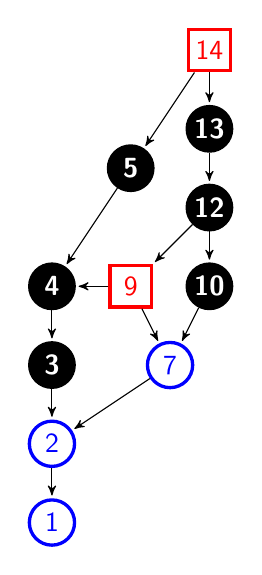
\begin{tikzpicture}[->,>=stealth',shorten >=1pt,auto,node distance=3cm,
  thick,main node/.style={circle,fill=blue!20,draw,font=\sffamily\Large\bfseries}]
  
  
  
  \node[arn_b] (a1) at (0,0) {1};
  \node[arn_b] (a2) at (0,1) {2};
  
  \node[arn_n] (a5) at (1,4.5) {5};
  \node[arn_n] (a13) at (2,5) {13};
  \node[arn_rs] (a14) at (2,6) {14};
  
  
  \node[arn_n] (a10) at (2,3) {10};
  \node[arn_b] (a7) at (1.5,2) {7};
  \node[arn_n] (a3) at (0,2) {3};
  
  \node[arn_rs] (a9) at (1,3) {9};
  \node[arn_n] (a12) at (2,4) {12};
  \node[arn_n] (a4) at (0,3) {4};
  
  %   Alice history
  \path[thin] (a14) edge (a5);
  \path[thin] (a5) edge (a4);
  \path[thin] (a4) edge (a3);
  \path[thin] (a3) edge (a2);
  \path[thin] (a2) edge (a1);
  \path[thin] (a9) edge (a4);
  \path[thin] (a7) edge (a2);
%   both history
  \path[thin] (a14) edge (a13);
  \path[thin] (a13) edge (a12);
  \path[thin] (a12) edge (a9);
  \path[thin] (a12) edge (a10);
  
  \path[thin] (a9) edge (a7);
  \path[thin] (a10) edge (a7);
  \end{tikzpicture}
  \caption{deal with bloomfilters}
\end{minipage}
 \begin{minipage}{0.3\textwidth}
 \centering
 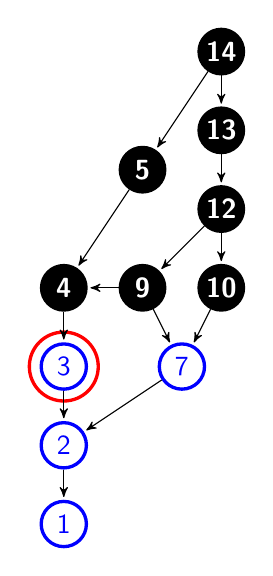
\begin{tikzpicture}[->,>=stealth',shorten >=1pt,auto,node distance=3cm,
  thick,main node/.style={circle,fill=blue!20,draw,font=\sffamily\Large\bfseries}]
  
  

  \node[arn_rb] (emph) at (0,2) {};
  \node[arn_b] (a1) at (0,0) {1};
  \node[arn_b] (a2) at (0,1) {2};
  
  \node[arn_n] (a5) at (1,4.5) {5};
  \node[arn_n] (a13) at (2,5) {13};
  \node[arn_n] (a14) at (2,6) {14};
  
  
  \node[arn_n] (a10) at (2,3) {10};
  \node[arn_b] (a7) at (1.5,2) {7};
  \node[arn_b] (a3) at (0,2) {3};
  
  \node[arn_n] (a9) at (1,3) {9};
  \node[arn_n] (a12) at (2,4) {12};
  \node[arn_n] (a4) at (0,3) {4};
%   \node[cloud, fill=gray!20, cloud puffs=16, cloud puff arc= 100,minimum width=2em, minimum height=2em, aspect=1] (cloud) at (5,2) {};

  %   Alice history
  \path[thin] (a14) edge (a5);
  \path[thin] (a5) edge (a4);
  \path[thin] (a4) edge (a3);
  \path[thin] (a3) edge (a2);
  \path[thin] (a2) edge (a1);
  \path[thin] (a9) edge (a4);
  \path[thin] (a7) edge (a2);
%   both history
  \path[thin] (a14) edge (a13);
  \path[thin] (a13) edge (a12);
  \path[thin] (a12) edge (a9);
  \path[thin] (a12) edge (a10);
  
  \path[thin] (a9) edge (a7);
  \path[thin] (a10) edge (a7);
  \end{tikzpicture}
  \caption{deal with border}
\end{minipage}
\end{figure}
\begin{figure}[H]
  \begin{minipage}{0.3\textwidth}
  \centering
 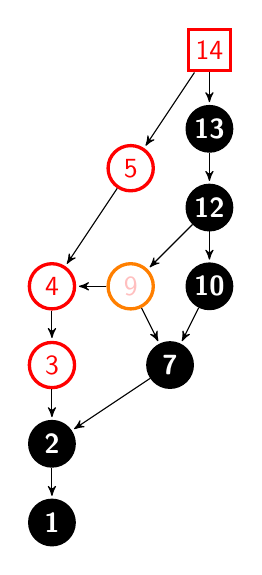
\begin{tikzpicture}[->,>=stealth',shorten >=1pt,auto,node distance=3cm,
  thick,main node/.style={circle,fill=blue!20,draw,font=\sffamily\Large\bfseries}]
  
  
  \node[arn_n] (a1) at (0,0) {1};
  \node[arn_n] (a2) at (0,1) {2};
  
  \node[arn_r] (a5) at (1,4.5) {5};
  \node[arn_n] (a13) at (2,5) {13};
  \node[arn_rs] (a14) at (2,6) {14};
  
  
  \node[arn_n] (a10) at (2,3) {10};
  \node[arn_n] (a7) at (1.5,2) {7};
  \node[arn_r] (a3) at (0,2) {3};
  
  \node[arn_t] (a9) at (1,3) {9};
  \node[arn_n] (a12) at (2,4) {12};
  \node[arn_r] (a4) at (0,3) {4};
%   \node[cloud, fill=gray!20, cloud puffs=16, cloud puff arc= 100,minimum width=2em, minimum height=2em, aspect=1] (cloud) at (5,2) {};

  %   Alice history
  \path[thin] (a14) edge (a5);
  \path[thin] (a5) edge (a4);
  \path[thin] (a4) edge (a3);
  \path[thin] (a3) edge (a2);
  \path[thin] (a2) edge (a1);
  \path[thin] (a9) edge (a4);
  \path[thin] (a7) edge (a2);
%   both history
  \path[thin] (a14) edge (a13);
  \path[thin] (a13) edge (a12);
  \path[thin] (a12) edge (a9);
  \path[thin] (a12) edge (a10);
  
  \path[thin] (a9) edge (a7);
  \path[thin] (a10) edge (a7);
  \end{tikzpicture}
  \caption{explore}
\end{minipage}
\begin{minipage}{0.3\textwidth}
  \centering
 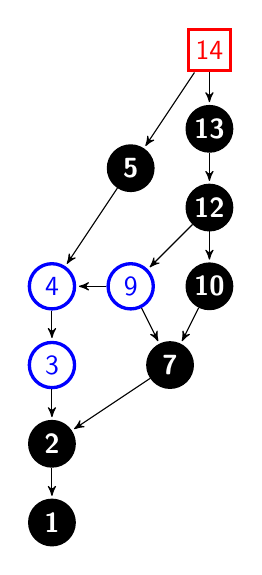
\begin{tikzpicture}[->,>=stealth',shorten >=1pt,auto,node distance=3cm,
  thick,main node/.style={circle,fill=blue!20,draw,font=\sffamily\Large\bfseries}]
  
  
  \node[arn_n] (a1) at (0,0) {1};
  \node[arn_n] (a2) at (0,1) {2};
  
  \node[arn_n] (a5) at (1,4.5) {5};
  \node[arn_n] (a13) at (2,5) {13};
  \node[arn_rs] (a14) at (2,6) {14};
  
  
  \node[arn_n] (a10) at (2,3) {10};
  \node[arn_n] (a7) at (1.5,2) {7};
  \node[arn_b] (a3) at (0,2) {3};
  
  \node[arn_b] (a9) at (1,3) {9};
  \node[arn_n] (a12) at (2,4) {12};
  \node[arn_b] (a4) at (0,3) {4};
%   \node[cloud, fill=gray!20, cloud puffs=16, cloud puff arc= 100,minimum width=2em, minimum height=2em, aspect=1] (cloud) at (5,2) {};

  %   Alice history
  \path[thin] (a14) edge (a5);
  \path[thin] (a5) edge (a4);
  \path[thin] (a4) edge (a3);
  \path[thin] (a3) edge (a2);
  \path[thin] (a2) edge (a1);
  \path[thin] (a9) edge (a4);
  \path[thin] (a7) edge (a2);
%   both history
  \path[thin] (a14) edge (a13);
  \path[thin] (a13) edge (a12);
  \path[thin] (a12) edge (a9);
  \path[thin] (a12) edge (a10);
  
  \path[thin] (a9) edge (a7);
  \path[thin] (a10) edge (a7);
  \end{tikzpicture}
  \caption{deal with bloomfilters}
\end{minipage}
\begin{minipage}{0.3\textwidth}
  \centering
 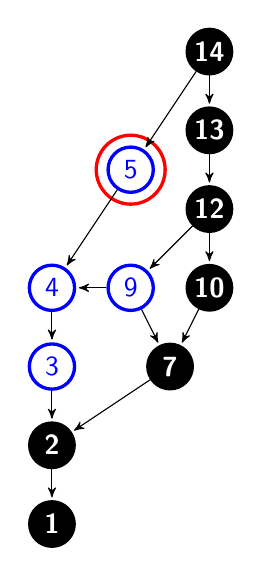
\begin{tikzpicture}[->,>=stealth',shorten >=1pt,auto,node distance=3cm,
  thick,main node/.style={circle,fill=blue!20,draw,font=\sffamily\Large\bfseries}]
  
  \node[arn_rb] (emph) at (1,4.5) {};
  \node[arn_n] (a1) at (0,0) {1};
  \node[arn_n] (a2) at (0,1) {2};
  
  \node[arn_b] (a5) at (1,4.5) {5};
  \node[arn_n] (a13) at (2,5) {13};
  \node[arn_n] (a14) at (2,6) {14};
  
  
  \node[arn_n] (a10) at (2,3) {10};
  \node[arn_n] (a7) at (1.5,2) {7};
  \node[arn_b] (a3) at (0,2) {3};
  
  \node[arn_b] (a9) at (1,3) {9};
  \node[arn_n] (a12) at (2,4) {12};
  \node[arn_b] (a4) at (0,3) {4};
%   \node[cloud, fill=gray!20, cloud puffs=16, cloud puff arc= 100,minimum width=2em, minimum height=2em, aspect=1] (cloud) at (5,2) {};

  %   Alice history
  \path[thin] (a14) edge (a5);
  \path[thin] (a5) edge (a4);
  \path[thin] (a4) edge (a3);
  \path[thin] (a3) edge (a2);
  \path[thin] (a2) edge (a1);
  \path[thin] (a9) edge (a4);
  \path[thin] (a7) edge (a2);
%   both history
  \path[thin] (a14) edge (a13);
  \path[thin] (a13) edge (a12);
  \path[thin] (a12) edge (a9);
  \path[thin] (a12) edge (a10);
  
  \path[thin] (a9) edge (a7);
  \path[thin] (a10) edge (a7);
  \end{tikzpicture}
  \caption{deal with borders}
\end{minipage}
\end{figure}
\begin{figure}[H]
 
\begin{minipage}{0.3\textwidth}
  \centering
 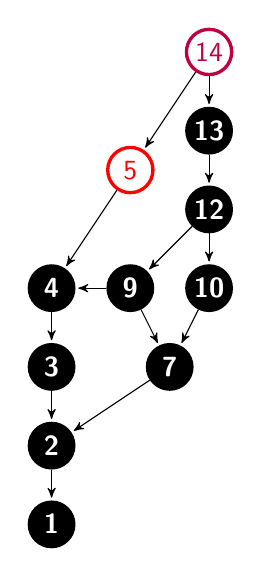
\begin{tikzpicture}[->,>=stealth',shorten >=1pt,auto,node distance=3cm,
  thick,main node/.style={circle,fill=blue!20,draw,font=\sffamily\Large\bfseries}]
  
  
  \node[arn_n] (a1) at (0,0) {1};
  \node[arn_n] (a2) at (0,1) {2};
  
  \node[arn_r] (a5) at (1,4.5) {5};
  \node[arn_n] (a13) at (2,5) {13};
  \node[arn_pu] (a14) at (2,6) {14};
  
  
  \node[arn_n] (a10) at (2,3) {10};
  \node[arn_n] (a7) at (1.5,2) {7};
  \node[arn_n] (a3) at (0,2) {3};
  
  \node[arn_n] (a9) at (1,3) {9};
  \node[arn_n] (a12) at (2,4) {12};
  \node[arn_n] (a4) at (0,3) {4};
%   \node[cloud, fill=gray!20, cloud puffs=16, cloud puff arc= 100,minimum width=2em, minimum height=2em, aspect=1] (cloud) at (5,2) {};

  %   Alice history
  \path[thin] (a14) edge (a5);
  \path[thin] (a5) edge (a4);
  \path[thin] (a4) edge (a3);
  \path[thin] (a3) edge (a2);
  \path[thin] (a2) edge (a1);
  \path[thin] (a9) edge (a4);
  \path[thin] (a7) edge (a2);
%   both history
  \path[thin] (a14) edge (a13);
  \path[thin] (a13) edge (a12);
  \path[thin] (a12) edge (a9);
  \path[thin] (a12) edge (a10);
  
  \path[thin] (a9) edge (a7);
  \path[thin] (a10) edge (a7);
  \end{tikzpicture}
  \caption{explore}
\end{minipage}
\begin{minipage}{0.3\textwidth}
  \centering
 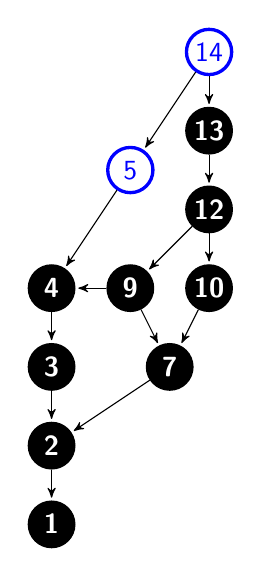
\begin{tikzpicture}[->,>=stealth',shorten >=1pt,auto,node distance=3cm,
  thick,main node/.style={circle,fill=blue!20,draw,font=\sffamily\Large\bfseries}]
  
  
  \node[arn_n] (a1) at (0,0) {1};
  \node[arn_n] (a2) at (0,1) {2};
  
  \node[arn_b] (a5) at (1,4.5) {5};
  \node[arn_n] (a13) at (2,5) {13};
  \node[arn_b] (a14) at (2,6) {14};
  
  
  \node[arn_n] (a10) at (2,3) {10};
  \node[arn_n] (a7) at (1.5,2) {7};
  \node[arn_n] (a3) at (0,2) {3};
  
  \node[arn_n] (a9) at (1,3) {9};
  \node[arn_n] (a12) at (2,4) {12};
  \node[arn_n] (a4) at (0,3) {4};
%   \node[cloud, fill=gray!20, cloud puffs=16, cloud puff arc= 100,minimum width=2em, minimum height=2em, aspect=1] (cloud) at (5,2) {};

  %   Alice history
  \path[thin] (a14) edge (a5);
  \path[thin] (a5) edge (a4);
  \path[thin] (a4) edge (a3);
  \path[thin] (a3) edge (a2);
  \path[thin] (a2) edge (a1);
  \path[thin] (a9) edge (a4);
  \path[thin] (a7) edge (a2);
%   both history
  \path[thin] (a14) edge (a13);
  \path[thin] (a13) edge (a12);
  \path[thin] (a12) edge (a9);
  \path[thin] (a12) edge (a10);
  
  \path[thin] (a9) edge (a7);
  \path[thin] (a10) edge (a7);
  \end{tikzpicture}
  \caption{deal with bloomfilters}
\end{minipage}
\begin{minipage}{0.3\textwidth}
  \centering
 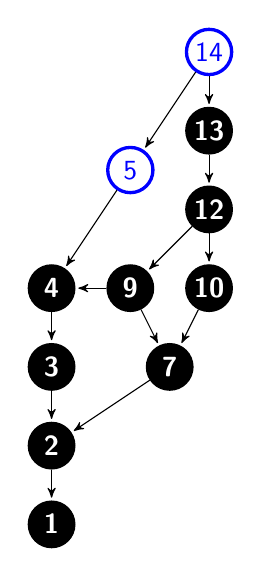
\begin{tikzpicture}[->,>=stealth',shorten >=1pt,auto,node distance=3cm,
  thick,main node/.style={circle,fill=blue!20,draw,font=\sffamily\Large\bfseries}]
  
  
  \node[arn_n] (a1) at (0,0) {1};
  \node[arn_n] (a2) at (0,1) {2};
  
  \node[arn_b] (a5) at (1,4.5) {5};
  \node[arn_n] (a13) at (2,5) {13};
  \node[arn_b] (a14) at (2,6) {14};
  
  
  \node[arn_n] (a10) at (2,3) {10};
  \node[arn_n] (a7) at (1.5,2) {7};
  \node[arn_n] (a3) at (0,2) {3};
  
  \node[arn_n] (a9) at (1,3) {9};
  \node[arn_n] (a12) at (2,4) {12};
  \node[arn_n] (a4) at (0,3) {4};
%   \node[cloud, fill=gray!20, cloud puffs=16, cloud puff arc= 100,minimum width=2em, minimum height=2em, aspect=1] (cloud) at (5,2) {};

  %   Alice history
  \path[thin] (a14) edge (a5);
  \path[thin] (a5) edge (a4);
  \path[thin] (a4) edge (a3);
  \path[thin] (a3) edge (a2);
  \path[thin] (a2) edge (a1);
  \path[thin] (a9) edge (a4);
  \path[thin] (a7) edge (a2);
%   both history
  \path[thin] (a14) edge (a13);
  \path[thin] (a13) edge (a12);
  \path[thin] (a12) edge (a9);
  \path[thin] (a12) edge (a10);
  
  \path[thin] (a9) edge (a7);
  \path[thin] (a10) edge (a7);
  \end{tikzpicture}
  \caption{deal with borders}
\end{minipage}
\end{figure}
\end{document}
% p3.  Research Subject
% - manque un petit paragraphe: pour expliquer ce que tu as fait pendant ton stage: expliquer ton titre: immutable DAGs, expliquer le "cost modèle" du graphe (écriture rapide, accès aux prédécesseurs rapides, les graphes ne peuvent que grossir), expliquer la synchronisation dans ce cas est un calcul de différence, et qu'il va falloir qu'on puisse calculer rapidement si un élément est dans le passé de 2 éléments.
% - manque un paragraphe pour expliquer quelle approche tu as suivi: expérimentation sur les vector clocks, sur les bloom filters, implémentation d'un algo de graph client/serveur "stateless" qui est optimisée pour des différences petits (ie. complexité relative a la taille de la différence). Evaluation en le comparant à de vrais systèmes (je dois t'aider pour instrumenter Git, mais ça serait bien de trouver des trucs qui synchronisent des Merkle tree si on a du temps, sinon tant pis)


% p7. Chapter 3

% revoir l'organisation de la section

% 3. faire un para entier sur ton algo de génération de graphe aléatoire
% stats manquantes: nombre d'éléments vérifiant l'égalité quand y 1 seul BCA
% 
% p8 Algo
% 
% (normaliser aussi les utilisations de successors, predecessors)
% 
% structure de la suite:

% Dernier point. Je me demande si ça serait pas plus simple de dire très tôt (par exemple dans l'intro du chapitre 2) qu'on travaille sur des graphes immutables, et que du coup on fixe un graphe global G une fois pour toute. Ensuite l'état des process c'est juste leur heads (et leur graphes c'est la fermeture transitive des têtes \downarrow(H) ou un truc du genre). Ça permettait d'être plus clair sur tes fonction "Ancestor" (qui n'est jamais vraiment défini dans ton rapport). Qu'en penses tu ?

% - p2: intro and context:
% NetOS -> Ocaml Labs -> Mirage -> Irmin
% 

% Rajoute des Figures~\ref{xxx} a chaque fois que tu cites une figure (c'est valable dans tout le document)
% prop1 et 2: rajoute des références (et/ou des preuves)
 

% dire qu'on peut écrire BF plutôt que Bloom filter et l'utiliser dans le rapport
%
% proposition 3: manque la ref
% 

% 1. et 2. -> manque les refs
% 
% % % % % % % % % % % % % % % % % % % % % % % % % % % 
% pour le coeur de la partie, je pense qu'il faut:
% - expliquer la figure 3.3
% - donner le type des fonctions
% - donner les invariants
% - pointer vers l'appendix pour avoir plus de détails (ou le code) mais si les invariants sont suffisamment clairs, c'est même pas sur qu'on en est besoin
% 
% p14. rajouter quelque part des explications sur le choix de la taille des slices. Rajouter une reference a cette section a la fin de la 1er phrase de 3.3.2
% 
% p15. "having a false positive in a border is very rare" -> si les frontères sont pleines, c'est pareil que pour les BF des slices, du coup je suis pas fan de cette phrase. Peut-être rajouter un example pour montrer les ravages que peuvent causer un faux positif sur un frontière (et dire que c'est un cas pathologique vraiment compliqué a construire)
% 
% fig 3.15: sympa, mais je rajouterais un peu plus d'infos dans les captions (ie. a chaque fois, dire quels sont les noeuds sélectionnés)
% 
% manque une section 3.3.3 sur comment borner les frontières et la liste des slices (le client a une mémoire bornée) et que le serveur n'a pas besoin de garder d'état en mémoire (le serveur aussi a une mémoire bornée)
% 
% 3.4 évaluation: c'est tout vide!! :p